% Options for packages loaded elsewhere
\PassOptionsToPackage{unicode}{hyperref}
\PassOptionsToPackage{hyphens}{url}
%
\documentclass[
]{book}
\usepackage{lmodern}
\usepackage{amssymb,amsmath}
\usepackage{ifxetex,ifluatex}
\ifnum 0\ifxetex 1\fi\ifluatex 1\fi=0 % if pdftex
  \usepackage[T1]{fontenc}
  \usepackage[utf8]{inputenc}
  \usepackage{textcomp} % provide euro and other symbols
\else % if luatex or xetex
  \usepackage{unicode-math}
  \defaultfontfeatures{Scale=MatchLowercase}
  \defaultfontfeatures[\rmfamily]{Ligatures=TeX,Scale=1}
\fi
% Use upquote if available, for straight quotes in verbatim environments
\IfFileExists{upquote.sty}{\usepackage{upquote}}{}
\IfFileExists{microtype.sty}{% use microtype if available
  \usepackage[]{microtype}
  \UseMicrotypeSet[protrusion]{basicmath} % disable protrusion for tt fonts
}{}
\makeatletter
\@ifundefined{KOMAClassName}{% if non-KOMA class
  \IfFileExists{parskip.sty}{%
    \usepackage{parskip}
  }{% else
    \setlength{\parindent}{0pt}
    \setlength{\parskip}{6pt plus 2pt minus 1pt}}
}{% if KOMA class
  \KOMAoptions{parskip=half}}
\makeatother
\usepackage{xcolor}
\IfFileExists{xurl.sty}{\usepackage{xurl}}{} % add URL line breaks if available
\IfFileExists{bookmark.sty}{\usepackage{bookmark}}{\usepackage{hyperref}}
\hypersetup{
  pdftitle={Hizkuntzaren Didaktika (Lehen Hezkuntza) V-2020/09},
  hidelinks,
  pdfcreator={LaTeX via pandoc}}
\urlstyle{same} % disable monospaced font for URLs
\usepackage{longtable,booktabs}
% Correct order of tables after \paragraph or \subparagraph
\usepackage{etoolbox}
\makeatletter
\patchcmd\longtable{\par}{\if@noskipsec\mbox{}\fi\par}{}{}
\makeatother
% Allow footnotes in longtable head/foot
\IfFileExists{footnotehyper.sty}{\usepackage{footnotehyper}}{\usepackage{footnote}}
\makesavenoteenv{longtable}
\usepackage{graphicx}
\makeatletter
\def\maxwidth{\ifdim\Gin@nat@width>\linewidth\linewidth\else\Gin@nat@width\fi}
\def\maxheight{\ifdim\Gin@nat@height>\textheight\textheight\else\Gin@nat@height\fi}
\makeatother
% Scale images if necessary, so that they will not overflow the page
% margins by default, and it is still possible to overwrite the defaults
% using explicit options in \includegraphics[width, height, ...]{}
\setkeys{Gin}{width=\maxwidth,height=\maxheight,keepaspectratio}
% Set default figure placement to htbp
\makeatletter
\def\fps@figure{htbp}
\makeatother
\setlength{\emergencystretch}{3em} % prevent overfull lines
\providecommand{\tightlist}{%
  \setlength{\itemsep}{0pt}\setlength{\parskip}{0pt}}
\setcounter{secnumdepth}{5}
\usepackage{booktabs}
\usepackage{amsthm}
\usepackage[basque]{babel}
\makeatletter
\def\thm@space@setup{%
  \thm@preskip=8pt plus 2pt minus 4pt
  \thm@postskip=\thm@preskip
}
\makeatother
\usepackage[]{natbib}
\bibliographystyle{apalike}

\title{Hizkuntzaren Didaktika (Lehen Hezkuntza) V-2020/09}
\author{true}
\date{2020/2021}

\begin{document}
\maketitle

{
\setcounter{tocdepth}{1}
\tableofcontents
}
\hypertarget{hizkuntzaren-didaktika-lh-apunteak-20202021}{%
\chapter*{Hizkuntzaren Didaktika (LH): apunteak 2020/2021}\label{hizkuntzaren-didaktika-lh-apunteak-20202021}}
\addcontentsline{toc}{chapter}{Hizkuntzaren Didaktika (LH): apunteak 2020/2021}

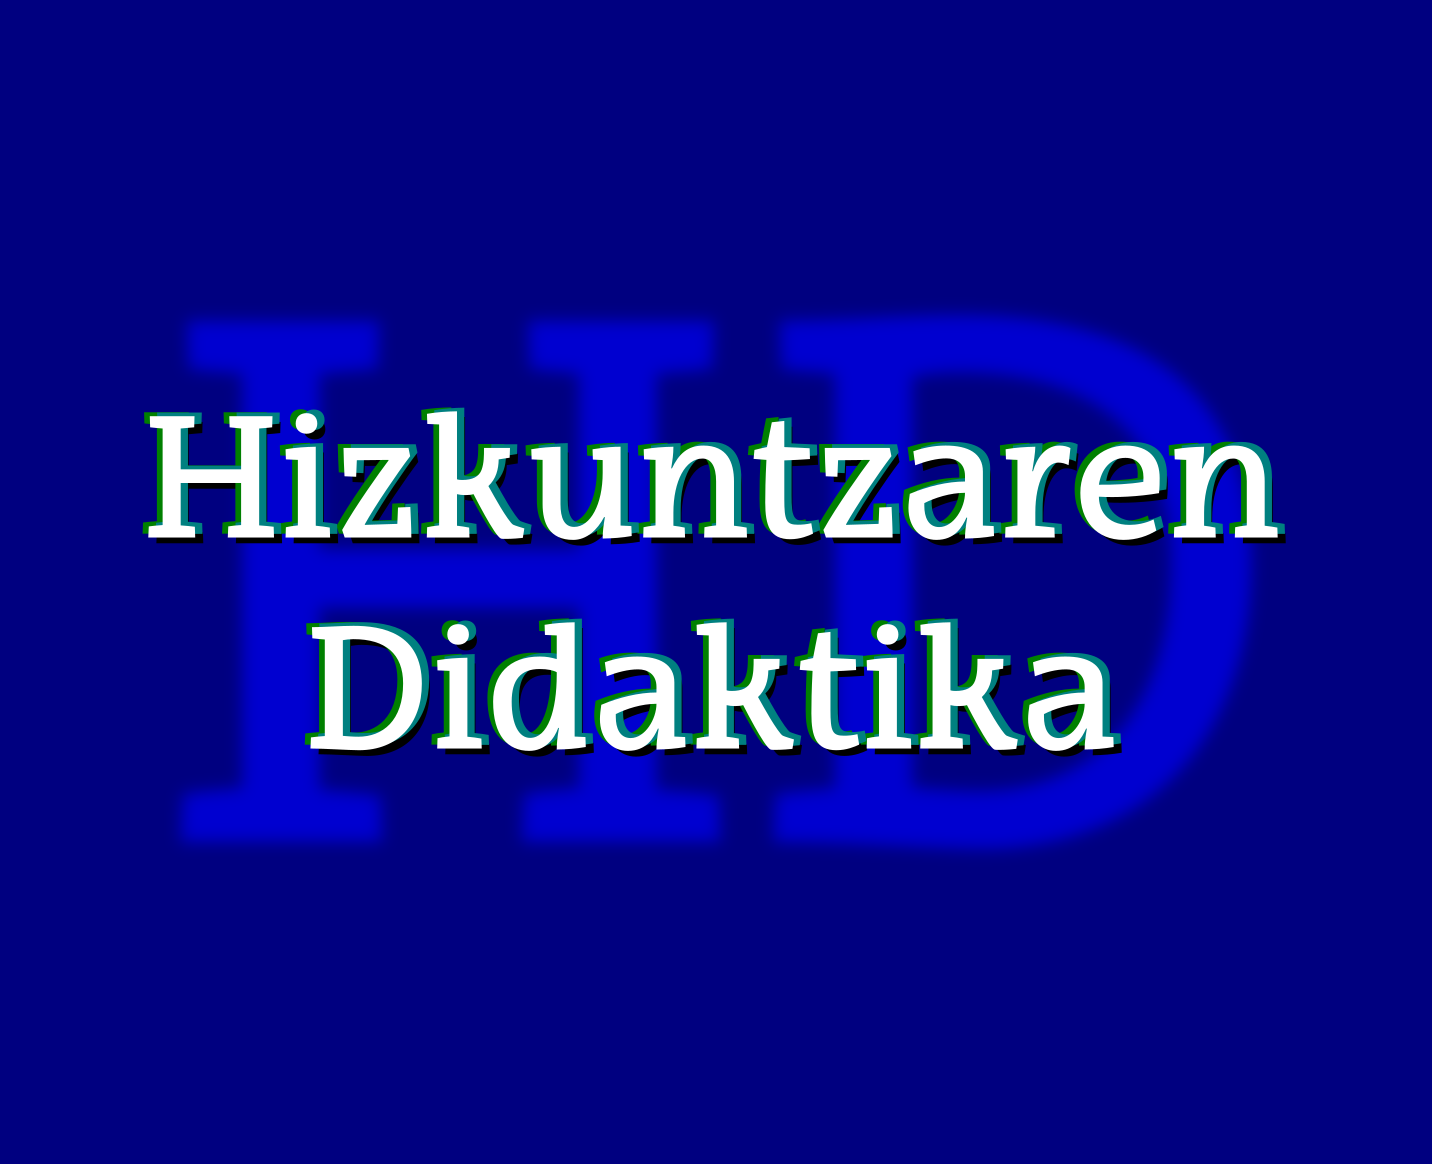
\includegraphics{assets/azala.png}

\hypertarget{jakingarriak}{%
\section*{Jakingarriak}\label{jakingarriak}}
\addcontentsline{toc}{section}{Jakingarriak}

Hemen duzun dokumentuak ikasgairako beharko dituzun elementu gehienak editu berton edo estekatuta:

\begin{enumerate}
\def\labelenumi{\arabic{enumi}.}
\tightlist
\item
  Ikagaiaren gida eta nirekin harremanetan paratzeko argigarriak
\item
  \href{https://www.ehu.eus/eu/web/hld-dll/ikasgaiak?p_redirect=consultaAsignatura\&p_anyo_acad=20200\&p_ciclo=X\&p_curso=3\&p_cod_asignatura=25868\&p_cod_plan=GPRIMA30\&p_cod_centro=354}{Gida ofiziala} (kapitulu honetan)
\item
  Kapitulurik kapitulu, apunteak, diapositibetarako estekak eta bakoitzaren amaieran bibliografia eta ariketak aurkituko dituzu.
\end{enumerate}

Goiko ``download'' botoian PDF(?) edo EPUB formatuan ere jaits dezakezue gida.

\textbf{Irakaslea}: Juan Abasolo

Nirekin kontaktuan jartzeko, Telegram erabiltzea gomendatzen dizuet, korreoak eta abar baino eraginkorragoa baita. Hala ere, batzuetan ibili ez arren eta biltegiratze gaitasun urria badu ere, denok dugunez UPV/EHUko korreoa, komunikazio ofizialak bertatik egin behar ditugu. Aurten zuen banaketa zerrenda ez dabil.

\begin{itemize}
\tightlist
\item
  Telegram: {[}abildua{]} JuanAbasolo
\item
  emaila: juan {[}puntu{]} abasolo {[}abildua{]} ehu {[}puntu{]} eus
\item
  Bulegoa: 3S40B
\item
  Tutoretzak: \url{https://labur.eus/JAbasolo-tutoretzak}\\
  Aurretik norbaitekin hitzordua egiten dudanean hor ere agertuko da. Fakultatekoa edo GAURrekoa bitaminizatua, beraz.
\end{itemize}

\textbf{Ikastaldea}: LH 32, 3. maila, lehenengo lauhilekoan.

Balibideak partekatzeko, eztabaida informaletarako eta azken momentuko informazio edo premietarako-eta proposatzen dizuedan foroa \href{https://t.me/joinchat/CheQnxAMdJ206V3d4kDLkw}{hemen} duzue. Hori erabiltzeko Telegrameko kontua egin beharko duzue (telefonoan edo ordenagailuan erabil dezakezue). Whatsappeko taldeen antzerako kudeaketa du, baina inori telefono zenbakia eman beharrik gabe.

Ikasgaiaren lehenengo zatian ia ez dugu erabiliko Moodle-n oinarritutako plataformarik.

\textbf{Ikasgaia}: Gida hau UPV/EHUko web \href{https://www.ehu.eus/eu/lehen-hezkuntzako-gradua-bizkaia/kreditu-eta-irakasgaiak?p_redirect=consultaAsignatura\&p_cod_proceso=egr\&p_anyo_acad=20180\&p_ciclo=X\&p_curso=3\&p_cod_asignatura=25868}{orritik bertatik} hartutakoa da, beraz, irakurri eta aztertuta baduzu, hurrengo pausura iragan.

\textbf{Proiektua}:

\href{syllabusa/Syllabus_HDLH20-V1-1.pdf}{
\includegraphics{assets/pdficon.png}}

\hypertarget{hizkuntzaren-eta-literaturaren-didaktika---25868}{%
\chapter*{Hizkuntzaren eta Literaturaren Didaktika - 25868}\label{hizkuntzaren-eta-literaturaren-didaktika---25868}}
\addcontentsline{toc}{chapter}{Hizkuntzaren eta Literaturaren Didaktika - 25868}

\begin{itemize}
\item
  Ikastegia\\
  Bilboko Hezkuntza Fakultatea
\item
  Titulazioa\\
  Lehen Hezkuntzako Gradua
\item
  Ikasturtea\\
  2020/21
\item
  Maila\\
  3
\item
  Kreditu kopurua\\
  10
\item
  Hizkuntzak\\
  Euskara
\end{itemize}

\hypertarget{irakaskuntza}{%
\section*{Irakaskuntza}\label{irakaskuntza}}
\addcontentsline{toc}{section}{Irakaskuntza}

\begin{longtable}[]{@{}lll@{}}
\toprule
\begin{minipage}[b]{0.18\columnwidth}\raggedright
Irakaskuntza mota\strut
\end{minipage} & \begin{minipage}[b]{0.25\columnwidth}\raggedright
Ikasgelako eskola-orduak\strut
\end{minipage} & \begin{minipage}[b]{0.48\columnwidth}\raggedright
Ikaslearen ikasgelaz kanpoko jardueren orduak\strut
\end{minipage}\tabularnewline
\midrule
\endhead
\begin{minipage}[t]{0.18\columnwidth}\raggedright
Magistrala\strut
\end{minipage} & \begin{minipage}[t]{0.25\columnwidth}\raggedright
20\strut
\end{minipage} & \begin{minipage}[t]{0.48\columnwidth}\raggedright
30\strut
\end{minipage}\tabularnewline
\begin{minipage}[t]{0.18\columnwidth}\raggedright
Gelako p.\strut
\end{minipage} & \begin{minipage}[t]{0.25\columnwidth}\raggedright
80\strut
\end{minipage} & \begin{minipage}[t]{0.48\columnwidth}\raggedright
120\strut
\end{minipage}\tabularnewline
\bottomrule
\end{longtable}

\hypertarget{irakaskuntza-gida}{%
\section*{Irakaskuntza-gida}\label{irakaskuntza-gida}}
\addcontentsline{toc}{section}{Irakaskuntza-gida}

\hypertarget{helburuak}{%
\subsection*{Helburuak}\label{helburuak}}
\addcontentsline{toc}{subsection}{Helburuak}

\begin{enumerate}
\def\labelenumi{\Alph{enumi})}
\tightlist
\item
  Hizkuntzen eta literaturaren eskolako curriculuma ezagutzea, aztertzea eta balioestea, eta ahozko eta idatzizko hizkuntzaren irakaskuntzarako proposamen metodologikoak aztertzea eta ebaluatzea
\item
  Lehen Hezkuntzako curriculumean aurreikusitako erabilera arloei dagozkien ahozko eta idatzizko berbaldiak ulertzen eta sortzen irakasteko estrategiak menderatzea
\item
  Ahozko edo idatzizko hizkuntzaren garapena sustatzeko sekuentzia didaktikoak diseinatzea, Lehen Hezkuntzako ikasgeletan aplikatzeko eta ikasleen hizkuntza-gaitasunen garapena bermatuko dituzten sekuentzia berriak diseinatu ahal izateko
\item
  Ikasleari oinarrizko ezagutzak ematea bere literatur prestakuntza eta etorkizunean izango dituen ikasleena osatzeko, eta Haur eta Gazte Literaturaren genero eta kontzeptuei buruzko hausnarketa kritikoak egiteko
\item
  Ikaslea literatur lanen irakurketa lantzeko eta bultzatzeko gai izatea, egile klasiko eta garaikideen lanak ezagutzea, eta bere sentikortasuna garatzea Haur eta Gazte Literaturaren prestakuntza-, sormen- eta estetika-balioez jabetzeko
\item
  Ikasleari gaitasuna ematea, didaktikako irizpideen arabera eta ahozko zein idatzizko literatur materialetatik abiatuta, irakaskuntza/ikaskuntako metodo, baliabide eta teknikak praktikan jartzeko, eta literatur irakurketak aukeratzeko irizpide egokien arabera
\end{enumerate}

\hypertarget{irakasgai-zerrenda}{%
\subsection*{Irakasgai-zerrenda}\label{irakasgai-zerrenda}}
\addcontentsline{toc}{subsection}{Irakasgai-zerrenda}

\begin{enumerate}
\def\labelenumi{\arabic{enumi}.}
\tightlist
\item
  GAIA.- Hizkuntzen eta literaturaren curriculumaren diseinua.\\
\end{enumerate}

\begin{itemize}
\tightlist
\item
  Curriculumaren kontzeptua\\
\item
  Hizkuntzaren curriculuma gaur egungo ikuspegi didaktikotik:\\
  - ezaugarriak
  - osatzen duten elementuak (helburuak, edukiak, metodologia, ebaluazioa)\\
\end{itemize}

\begin{enumerate}
\def\labelenumi{\arabic{enumi}.}
\setcounter{enumi}{1}
\tightlist
\item
  GAIA.- Ahozko hizkuntzaren didaktika.\\
\end{enumerate}

\begin{itemize}
\tightlist
\item
  Ahozkotasuna eta ulermena:\\
  - hitz egitea
  - mintzamenaren ulermena
  - hitz egitea eta entzutea gelaren egunerokoan\\
\item
  Mintzamena irakastea:\\
  - Irakasleen jarduerak ikasleen mintzamena garatzeko
  - Orientabideak LHko gelarako
\end{itemize}

\begin{enumerate}
\def\labelenumi{\arabic{enumi}.}
\setcounter{enumi}{2}
\tightlist
\item
  GAIA.- Idatzizko hizkuntzaren didaktika

  \begin{itemize}
  \tightlist
  \item
    Ahozko hizkuntza vs.~hizkuntza idatzia
  \item
    Zer da irakurtzea?
  \item
    Zer da idaztea?
  \item
    Hizkuntza idatziaren psikogenesia
  \item
    Irakurtzen-idazten irakasteko metodoak
  \item
    Erabaki didaktikoak.
  \item
    Proposamen didaktikoak: erabilera praktikoa eta erabilera zientifikoa.\\
  \end{itemize}
\item
  GAIA.- Hausnarketa metalinguistikorako didaktika LHn.

  \begin{itemize}
  \tightlist
  \item
    Tartehizkuntza eta errorea.
  \item
    Hizkuntzaren funtzioak umeen lengoian.
  \item
    Testua eta diskurtsoa
  \item
    Erroreak\\
  \end{itemize}
\item
  GAIA.- LHn ahozko eta idatzizko hizkuntza garatzeko sekuentzia didaktikoak programatzea.

  \begin{itemize}
  \tightlist
  \item
    Programak eta proposamen didaktikoak
  \item
    Atazak eta zereginak ahozko gaitasun komunikatiboa lantzeko
  \item
    Atazak eta zereginak idatzizko gaitasun komunikatiboa lantzeko\\
  \end{itemize}
\item
  GAIA.- Haur- eta gazte-literaturaren kontzeptua: teoriak, eztabaidak eta ikerketako ikuspegiak.
\item
  GAIA.- HGLren ezaugarriak eta generoak.
\item
  GAIA.- HGLren historiara hurbiltzea.
\item
  GAIA.- HGL eta eskola; irakurtzeko ohitura eta literatura-gaitasuna.
\item
  GAIA.- HGLa eta horren aplikazioa ikasgelan.
\end{enumerate}

\hypertarget{metodologia}{%
\subsection*{Metodologia}\label{metodologia}}
\addcontentsline{toc}{subsection}{Metodologia}

\begin{itemize}
\tightlist
\item
  Era indibidualean edota taldeka egindako lana
\item
  Ikaskuntza gidatua edota autonomoa
\item
  Ikaskuntza kooperatiboa
\item
  Jarduera teoriko-praktikoak
\end{itemize}

\hypertarget{ebaluazio-sistemak}{%
\subsection*{Ebaluazio-sistemak}\label{ebaluazio-sistemak}}
\addcontentsline{toc}{subsection}{Ebaluazio-sistemak}

\begin{itemize}
\tightlist
\item
  Azken Ebaluazioaren Sistema
\item
  Kalifikazioko tresnak eta ehunekoak:
\item
  Garatu beharreko proba idatzia (\%): 30
\item
  Test motatako proba (\%): 20
\item
  Banakako lanak (\%): 10
\item
  Talde lanak (arazoen ebazpenak, proiektuen diseinuak) (\%): 14
\item
  Lanen, irakurketen\ldots{} aurkezpena (\%): 10
\item
  DAL (\%): 16
\end{itemize}

\hypertarget{nahitaez-erabili-beharreko-materiala}{%
\subsection*{Nahitaez erabili beharreko materiala}\label{nahitaez-erabili-beharreko-materiala}}
\addcontentsline{toc}{subsection}{Nahitaez erabili beharreko materiala}

1513/2006 Errege Dekretua, 2006ko abenduaren 7koa, Lehen Hezkuntzako gutxieneko irakaskuntza ezartzen duena.

175/2007 DEKRETUA, urriaren 16koa, Euskal Autonomia Erkidegoko Oinarrizko Hezkuntzaren curriculuma sortu eta ezartzekoa. 218. gehigarria. 2007ko azaroak 13, EHAA.

• Testuen dossierra komentarioak egiteko
• Lehen Hezkuntzako hizkuntza ikasgaiaren testu liburuak
• Ordenagailua
• Testu liburuak

\hypertarget{bibliografia}{%
\subsection*{Bibliografia}\label{bibliografia}}
\addcontentsline{toc}{subsection}{Bibliografia}

\hypertarget{oinarrizko-bibliografia}{%
\subsubsection*{Oinarrizko bibliografia}\label{oinarrizko-bibliografia}}
\addcontentsline{toc}{subsubsection}{Oinarrizko bibliografia}

Abascal, D., Beneito, J.M. y Valero, F. (1997) Hablar y escuchar. Barcelona, Octaedro

Camps, A y Zayas, F. (Coords) (2006) Secuencias didácticas para aprender gramática.
Barcelona, Graó

Camps, A (coord) (2003) Secuencias didácticas para aprender a escribir. Barcelona, Graó.

Cassany, D. Enseñar lengua (1994) Barcelona, Graó.

COLOMER, T. (2009). Introducción a la literatura infantil y juvenil. Madril: Síntesis.

COLOMER, T.; Manresa, Mireia; Ramada Prieto, Lucas \& Lara Reyes López (eds.) (2018). Narrativas literarias en educación infantil y primaria. Madril: Síntesis.

CULLER, J. (2009). Breve introducción a la teoría de la literatura. Bartzelona: Crítica.

DURAN, T. (2009). Álbumes y otras lecturas. Análisis de los libros infantiles. Bartzelona: Octaedro.

ETXANIZ ERLE, X. eta J.M. López Gaseni (2011). XXI. mende hasierako haur eta gazte literatura. Arabako Foru Aldundia

ETXANIZ \& LOPEZ GASENI (2011): Egungo haur eta gazte literaturaren historia. Bilbo: UPV-EHU Argitalpen zerbitzua.

Fons Esteve, M. (2004) Leer y escribir para vivir. Barcelona, Graó.

IGERABIDE, J. K. (1993). Bularretik mintzora. Donostia: Erein.

JIMÉNEZ-PÉREZ, E. eta S. Fabregat Barrios (koords.) (2019). La literatura infantil y juvenil: investigaciones. Bartzelona: Octaedro.

LLUCH, G. eta F. Zayas (2015). Leer en el centro escolar. El plan de lectura. Bartzelona: Octaedro.

RETOLAZA, Iratxe (2017): Egungo euskal komikiaren historia. Bilbo: UPV-EHU Argitalpen Zerbitzua.

RODARI, G. (1979). Gramática de la fantasía. Madril: Avance.

Ruiz Bikandi, U., (2000) Didáctica de la segunda lengua en educación infantil y primaria. Madrid, Síntesis.

Palou, J Y Bosch, C. (Coords) (2005) La lengua oral en la escuela. Barcelona, Graó.

Sainz, M., (1996) ¿Irakurketa eta idazketa LHko bigarren eta hirugarren zikloetan¿, in HIK HASI, 10. zb.

Solé, I. Estrategias de lectura. Barcelona, Graó.

Wells, G., (1988) Aprender a leer y escribir. Barcelona, Laia

\hypertarget{gehiago-sakontzeko-bibliografia}{%
\subsubsection*{Gehiago sakontzeko bibliografia}\label{gehiago-sakontzeko-bibliografia}}
\addcontentsline{toc}{subsubsection}{Gehiago sakontzeko bibliografia}

Alcoba, S. (coord) (1999) La oralización. Barcelona, Ariel.

Bronckart, J. P. (1996), Activité Langagière, textes et discours. Lausanne.Delachaux et Niestlé.

Cassany, D. La cocina de la escritura. Barcelona Anagrama

Colomer, T. y Camps, A. (1996), Enseñar a leer, enseñar a comprender

González Fernández, A. (2004) Estrategias de comprensión lectora. Madrid, Síntesis.

Mendoza.A. (Coord) (2003) Didáctica de la lengua y la literatura. Madrid, Pearson Educación.

Pérez Rodríguez, M. A. (2004) Los nuevos lenguajes de la comunicación. Enseñar y aprender con los medios. Barcelona, Paidós.

Sanz Moreno, A.(2003) Cómo diseñar actividades de comprensión lectora. Departamento de Educación. Gobierno de Navarra

Schneuwly, B., (1992) ¿La concepción vygotskiana del lenguaje escrito¿ en Comunicación, Lenguaje y Educación, 16, pp.~49-59,

Teberosky, A. (1992), Aprendiendo a escribir. Barcelona, Horsori.

Tolchinsky, L. (1993); Aprendizaje del lenguaje escrito. Barcelona, Anthropos.

\hypertarget{aldizkariak}{%
\subsubsection*{Aldizkariak}\label{aldizkariak}}
\addcontentsline{toc}{subsubsection}{Aldizkariak}

TEXTOS de Didáctica de la lengua y la literatura.
ARTICLES de Did.actica de la lengua y la literatura
Lenguaje y textos

\hypertarget{taldeak}{%
\section*{Taldeak}\label{taldeak}}
\addcontentsline{toc}{section}{Taldeak}

\ldots{}

\hypertarget{ikasgelak}{%
\subsubsection*{Ikasgela(k)}\label{ikasgelak}}
\addcontentsline{toc}{subsubsection}{Ikasgela(k)}

\begin{itemize}
\tightlist
\item
  1S03G - IRAKASLEEN ESKOLAKO ERAIKIN HORIZONTALA - LEIOA
\end{itemize}

\hypertarget{teoriakoa-euskara---goizezerakutsiizkutatu-azpiorriak}{%
\subsection{32 Teoriakoa (Euskara - Goizez)Erakutsi/izkutatu azpiorriak}\label{teoriakoa-euskara---goizezerakutsiizkutatu-azpiorriak}}

\begin{longtable}[]{@{}llllll@{}}
\toprule
Asteak & Astelehena & Asteartea & Asteazkena & Osteguna & Ostirala\tabularnewline
\midrule
\endhead
1-1 & & & & 14:00-16:30 17:00-19:30 &\tabularnewline
5-5 & & & & 14:00-16:30 17:00-19:30 &\tabularnewline
16-16 & & 14:00-16:00 16:30-18:30 19:00-20:00 & & &\tabularnewline
19-19 & & 14:00-16:00 16:30-18:00 & & &\tabularnewline
\bottomrule
\end{longtable}

\hypertarget{irakasleak}{%
\subsubsection*{Irakasleak}\label{irakasleak}}
\addcontentsline{toc}{subsubsection}{Irakasleak}

\begin{itemize}
\tightlist
\item
  \href{https://www.ehu.eus/eu/web/hld-dll/ikasgaiak?p_redirect=consultaTutorias\&p_anyo_acad=20200\&p_idp=351472}{ABASOLO ISASA, JUAN SEBASTIAN}
\item
  \href{https://www.ehu.eus/eu/web/hld-dll/ikasgaiak?p_redirect=consultaTutorias\&p_anyo_acad=20200\&p_idp=4636}{ROJO COBOS, FRANCISCO JAVIER}
\end{itemize}

\hypertarget{gelako-p.-1-euskara---goizezerakutsiizkutatu-azpiorriak}{%
\subsection{32 Gelako p.-1 (Euskara - Goizez)Erakutsi/izkutatu azpiorriak}\label{gelako-p.-1-euskara---goizezerakutsiizkutatu-azpiorriak}}

\begin{longtable}[]{@{}llllll@{}}
\toprule
Asteak & Astelehena & Asteartea & Asteazkena & Osteguna & Ostirala\tabularnewline
\midrule
\endhead
2-4 & 18:30-20:00 & & & 16:30-20:00 &\tabularnewline
6-10 & 18:30-20:00 & & & 16:30-20:00 &\tabularnewline
17-18 & & & 14:00-15:30 & & 16:00-17:30\tabularnewline
20-30 & & & 14:00-15:30 & & 16:00-17:30\tabularnewline
\bottomrule
\end{longtable}

\hypertarget{irakasleak-1}{%
\subsubsection*{Irakasleak}\label{irakasleak-1}}
\addcontentsline{toc}{subsubsection}{Irakasleak}

\begin{itemize}
\tightlist
\item
  \href{https://www.ehu.eus/eu/web/hld-dll/ikasgaiak?p_redirect=consultaTutorias\&p_anyo_acad=20200\&p_idp=351472}{ABASOLO, JUAN}
\item
  \href{https://www.ehu.eus/eu/web/hld-dll/ikasgaiak?p_redirect=consultaTutorias\&p_anyo_acad=20200\&p_idp=2768}{KORTAZAR URIARTE, JON BATTI}
\item
  \href{https://www.ehu.eus/eu/web/hld-dll/ikasgaiak?p_redirect=consultaTutorias\&p_anyo_acad=20200\&p_idp=4636}{ROJO COBOS, FRANCISCO JAVIER}
\end{itemize}

\hypertarget{ikasgela}{%
\subsubsection*{Ikasgela}\label{ikasgela}}
\addcontentsline{toc}{subsubsection}{Ikasgela}

\begin{itemize}
\tightlist
\item
  2S08M - IRAKASLEEN ESKOLAKO ERAIKIN HORIZONTALA - LEIOA
\end{itemize}

\hypertarget{testuingurua}{%
\chapter{Testuingurua}\label{testuingurua}}

\href{../Diapoak/01_Diap-testuingurua.html}{
\includegraphics{assets/badge.png}}

Hizkuntza Didaktikaz aritu aurretik, hizkuntza, didaktika honen objektua alegia, inguratzen duten ezaugarriez jardun beharra dugu.

\hypertarget{hizkuntza-desberdinek-egoera-desberdinak}{%
\section{Hizkuntza desberdinek egoera desberdinak}\label{hizkuntza-desberdinek-egoera-desberdinak}}

Begiratzen badugu zen zen egoera XX. mendera arte, ikusiko dugu eskolan gehien irakatsi diren hizkuntzak, hizkuntza handiak izan direla (Idiazabal, 2003; Martí eta beste, 2005).

Kontuan izan behar da XIX. mendeko estatu mugen sorrerak hizkuntza gutxituen presentzia eskolan erabat baztertu zuela, eskolak hizkuntza nagusia eta bakarra irakatsi behar zuen. \emph{Nazioa}\footnote{kultura, hizkuntza, etnia} eta \emph{estatua}\footnote{ofiziala, administratiboa} kontzeptuak bat egin ziren.

Hizkuntzak nazioak eta estatuak baino askoz ere ugariagoak dira, eta ez datoz bat lurraldeetako mugekin, gainera, hizkuntza asko estatu bat baino gehiagoko lurretan hitz egiten dira (euskara, gaztelania eta frantsesa adibide argiak dira).

\begin{quote}
El concepto de lengua no es preciso, ni las fronteras lingüísticas coinciden con las geográficas. En España se reconocen cuatro lenguas, pero hay otras más, desde el leonés, el bable o la fabla aragonesa, hasta las lenguas de los emigrantes o el caló. Así y todo, España es uno de los países lingüísticamente más homogéneos, pues tiene una lengua oficial y común, el español, que hablan y entienden la mayoría de sus ciudadanos.''
\end{quote}

\emph{\textbf{Santiago Trancón }}\url{https://www.lanuevacronica.com/lengua-nacion-estado}

\hypertarget{zer-da-hizkuntzaren-didaktika}{%
\section{Zer da Hizkuntzaren Didaktika}\label{zer-da-hizkuntzaren-didaktika}}

Jakintza eremu hau prozesu luze baten ondorioz finkatu da ikerketa eremu bakar gisa. Berez, eremu ezberdinetatik aztertua izan da \emph{hizkuntza} objektuaren didaktika: hizkuntzalaritzatik, pedagogiatik, filologiatik, politikatik eta abarretik.

Hizkuntzaren irakaskuntzak aspaldiko erroak ditu; hizkuntza bera zer den ulertzeko era bakoitzak irakasteko era edo filosofiaren bat ekarri baitu, horrela, aniztasun handia aurki dezakegu hizkuntzaren didaktikaren arloaren historian eta jardunean.

70eko hamarkadan has daiteke hizkuntzaren didaktikaz hitz egiten. Lehenago hizkuntzalaritza aplikatuaz hitz egiten zen, eta ordura arte psikologiako, soziologiako eta pedagogiako jakintzak alde batera uzten ziren.

\begin{quote}
Así (Galisson, 1986) podemos decir que la Didáctica de la Lengua dependió directamente de la Lingüística y que de ahí surgió la Lingüística Aplicada, la cual intentó responder ante todo a las cuestiones ¿Qué? y ¿Cómo?.

A continuación y bajo la ínfluencia de la Psicología Evolutiva, de la Psicología Educativa y de la Psicología Cognitiva, añadió una preocupación por la metodología.

Finalmente y del conjunto de una serie de disciplinas tales como las Ciencias del Lenguaje, de la Psicología, de la Sociedad y de la Educación surgiría con entidad propia la Didáctica de la Lengua y la Literatura que intenta responder a las preguntas: ¿Por qué enseñar lengua y Literatura?, ¿Qué enseñar?, ¿A quién enseñar?, ¿Cómo? Y ¿Dónde?

--\emph{López Valero}, 1998: 222
\end{quote}

Galdera horiei erantzuna emateko sortu zen \textbf{Hizkuntzaren Didaktika} diziplina hau honela defini dezakegu:

\begin{quote}
La Didáctica de la Lengua constituye un campo de conocimiento que tiene como objeto el complejo proceso de enseñar y aprender lenguas con el fin de mejorar las prácticas y adecuarlas a las situaciones cambiantes en que esta actividad se desarrolla

--Camps, Guasch y Ruiz Bikandi, 2010, p.~71
\end{quote}

Gogoratu ditzagun, beraz, azpimarratutako ideiak:

\emph{Ezagutza eremu bat da bere objektua hizkuntzak irakastea eta ikastea duena, jarduna hobetu eta egokitzea helburu}

\hypertarget{hizkuntzak-zergatik-galtzen-dira}{%
\section{Hizkuntzak zergatik galtzen dira?}\label{hizkuntzak-zergatik-galtzen-dira}}

Kanpoko indarren ondorioz: \textbf{Globalizazioa.} Sarritan kanpoko indarrak barnekoari eragiten dio. Hizkuntza indartsuak, aurrerapen soziala eta pertsonala, hizkuntza natiboak desagertu.

Barneko indarren ondorioz: \textbf{Estatu/nazio} kontzeptuaren eragina ulertu behar da (grikoa, behe-prusiera edo euskara bera, bakoitza bere historiarekin).

Moreno-Cabrerak (2008) horren azalpena ekskaintzen du hurrengoa azalduaz: Hizkuntza inperialistak hedatzeak homogeneotasun linguistikoa ekarri du eta ez aniztasuna, izan ere hiztunek euren hizkuntza natiboak baztertu dituzte edota ez dituzte zaindu behar bezala, sarritan pentsatu baitute hizkuntza horiek garapen eta aurrerapen sozialaren nahiz pertsonalaren kontra doazela. Era honetan, bost kontinenteetako hizkuntza internazionalek beste zenbait baztertu eta desagertarazi dituzte.

\hypertarget{bost-kontinenteetako-hizkuntzen-egoeraz}{%
\section{Bost kontinenteetako hizkuntzen egoeraz}\label{bost-kontinenteetako-hizkuntzen-egoeraz}}

Hurrengo taulak hizkuntzen egoera erakusten du, ikuskera administratibo-kauntitatibo batetik gehienbat.

\begin{longtable}[]{@{}lrrrrr@{}}
\caption{Hizkuntzen egoera administratiboa (Iturria:\href{https://www.ethnologue.com/}{ethnologue.com}).}\tabularnewline
\toprule
& Amerikak & Afrika & Europa & Asia & Ozeania\tabularnewline
\midrule
\endfirsthead
\toprule
& Amerikak & Afrika & Europa & Asia & Ozeania\tabularnewline
\midrule
\endhead
Instituzionala & 37 & 194 & 73 & 203 & 71\tabularnewline
Garatzeko bidean & 234 & 542 & 81 & 362 & 379\tabularnewline
Indartsua & 145 & 1026 & 31 & 856 & 421\tabularnewline
Arazoduna & 309 & 245 & 50 & 693 & 234\tabularnewline
Desagertzeko zorian & 339 & 131 & 51 & 187 & 208\tabularnewline
\bottomrule
\end{longtable}

Kontuan izan, hizkuntza instituzionalez ari garenean, ez garela ari 578 hizkuntzez. Kontinente guztietako gehiketak horretara eramango bagintuzke ere, Europako hizkuntza nagusiak dira Ameriketan, Afrikan, Asian eta Ozeanian hizkuntza instituzionalak; hala nola, ingelesa, gaztelania, frantsesa, portugesa eta neerlandera.

Hizkuntza minorizatuen gaineko testigantza batzuk Nathional Geographic-eko erreportai \href{http://www.nationalgeographic.com.es/mundo-ng/grandes-reportajes/lenguas-peligro-extincion_6174/26}{honetan}.

\hypertarget{hizkuntzen-egoera-eta-hizkuntzen-didaktikak}{%
\section{Hizkuntzen egoera eta hizkuntzen didaktikak}\label{hizkuntzen-egoera-eta-hizkuntzen-didaktikak}}

Lewisek 2005ean azaldu zuenez, bada ezaugarri zerrenda bat kontuan hartu beharrekoa:

\begin{itemize}
\tightlist
\item
  Hizkuntzaren transmisioa edo ondorengoetaratzea
\item
  Hiztun kopuru absolutua
\item
  Hiztun-portzentajea
\item
  Hizkuntzaren erabilera-eremu berrien sorrera
\item
  Alfabetatzerako eta hezkuntzarako materialak egotea (gramatikak, hiztegiak, idatzizko literatura, hedabideak\ldots)
\item
  Gobernu eta erakundeen babesa
\item
  Hiztunen jarrera
\item
  Hizkuntza dokumentatua egotea
\end{itemize}

\hypertarget{hizkuntza-gutxituak-irakatsi-beharraz-gain-indarberritu-ere-egin-behar-dira}{%
\section{Hizkuntza gutxituak: Irakatsi beharraz gain, indarberritu ere egin behar dira}\label{hizkuntza-gutxituak-irakatsi-beharraz-gain-indarberritu-ere-egin-behar-dira}}

\textbf{UNESCO}:\url{http://www.unesco.org/languages-atlas/es/atlasmap.html}

\begin{quote}
``INSTRUMENTO de ratificación de la Carta Europea de las Lenguas Regionales o Minoritarias, hecha en Estrasburgo el 5 de noviembre de 1992.

Los Estados miembros del Consejo de Europa, signatarios de la presente Carta, Considerando que la finalidad del Consejo de Europa es conseguir una unión más estrecha entre sus miembros, en articular para salvaguardar y promover los ideales y principios que son su patrimonio común; Considerando que la protección de las lenguas regionales o minoritarias históricas de Europa, de las que algunas corren el riesgo de desaparecer con el tiempo, contribuye al mantenimiento y al desarrollo de las tradiciones y la riqueza culturales de Europa.''

--Carta Europea de las Lenguas Minoritarias o Regionales

\emph{BOE, 2001}
\end{quote}

\begin{quote}
La Declaración es un texto necesario, tal como manifiestan sus Preliminares, para «corregir los desequilibrios lingüísticos de manera que aseguren el respeto y el pleno despliegue de todas las lenguas y que establezcan los principios de una paz lingüística planetaria justa y equitativa, como factor principal de la convivencia social».

La propia voluntad de universalismo de la Declaración comporta la corrección de los desequilibrios para que se asegure el respeto y el pleno desarrollo de todas las lenguas.

--Declaración Universal de Derechos Lingüísticos

\emph{1996, Bartzelona}
\end{quote}

\hypertarget{europako-erreferentzia-marko-bateratuak}{%
\subsection{Europako Erreferentzia Marko Bateratuak:}\label{europako-erreferentzia-marko-bateratuak}}

Gaitasunak, jarduera komunikatiboak, mailak, deskribatu eta zehazten ditu helburuak, edukiak eta ebaluazio-irizpideen oinarri gisa.Europako Kontseiluak hartutako erabakiak dira.

\hypertarget{ikastetxeko-hizkuntza-proiektuaren-bidez}{%
\subsection{Ikastetxeko Hizkuntza Proiektuaren bidez:}\label{ikastetxeko-hizkuntza-proiektuaren-bidez}}

Ikastetxeak duen identitatea kontuan izanik, hizkuntzaren aldetiko erabakiak hartzen dira bai alor pedagogikoan bai instituzionalean.

\hypertarget{adibideak}{%
\subsubsection{Adibideak:}\label{adibideak}}

Bideoa: \href{http://www.youtube.com/embed/iFEjAhnv3ys?rel=0}{Hizkuntz Proiektua guraso bilera}

\url{http://elblogdemiguelcalvillo.blogspot.com.es/2011/02/video-promocional-del-proyecto.html}

\url{http://elblogdemiguelcalvillo.blogspot.com.es/2011/04/proyecto-linguistico-de-centro-el-video.html}

\hypertarget{hizkuntza-programak}{%
\subsection{Hizkuntza Programak}\label{hizkuntza-programak}}

Irakasleek ikasleekin egin beharreko \textbf{jarduerak }dira, eta betebeharretako bat zentroan dauden hizkuntza ezberdinen gaineko kontzientzia piztea izan daiteke.

\hypertarget{munduko-eskola-batzuetan-nolako-programez-erantzuten-zaie-hizkuntza-gutxituei}{%
\subsection{Munduko eskola batzuetan nolako programez erantzuten zaie hizkuntza gutxituei?}\label{munduko-eskola-batzuetan-nolako-programez-erantzuten-zaie-hizkuntza-gutxituei}}

Adibide bi ikusi ditzakegu hurrengo bideoan, bata Hego Afrikako errepublikan eta bestea Mazedoniako errepublikan.

Bideoa: \href{http://www.youtube.com/embed/nPUMvUBuX00?rel=0}{Euronews Learning World - El bilingüismo en el mundo}

\hypertarget{irakaskuntzan}{%
\section{Irakaskuntzan}\label{irakaskuntzan}}

Txepetx

Hizkuntza bat \textbf{ikastean }hiru faktorek eragiten dutela dio, gainera, osagarriak dira eta lotura dute:

\begin{enumerate}
\def\labelenumi{\arabic{enumi}.}
\item
  \textbf{Motibazioak}: Hizkuntza bat ikastera daramaten arrazoi, nahi edo interesak
\item
  \textbf{Ezagutzak}: Hizkuntzaren funtzionamendua ulertzeko gaitasuna edo prozesua.
\item
  \textbf{Erabilerak}.
\end{enumerate}

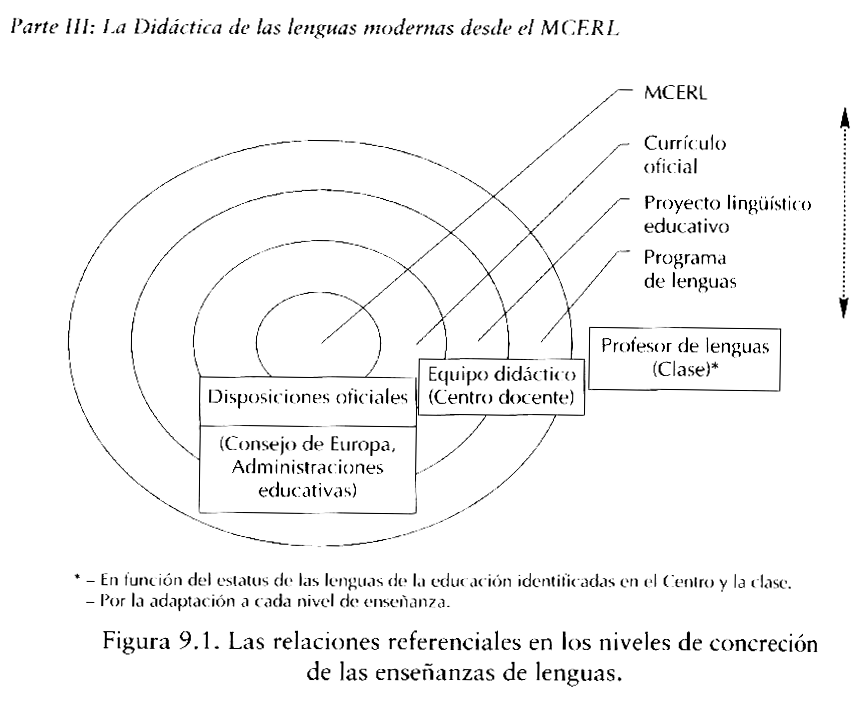
\includegraphics{assets/01_01-HD.png}

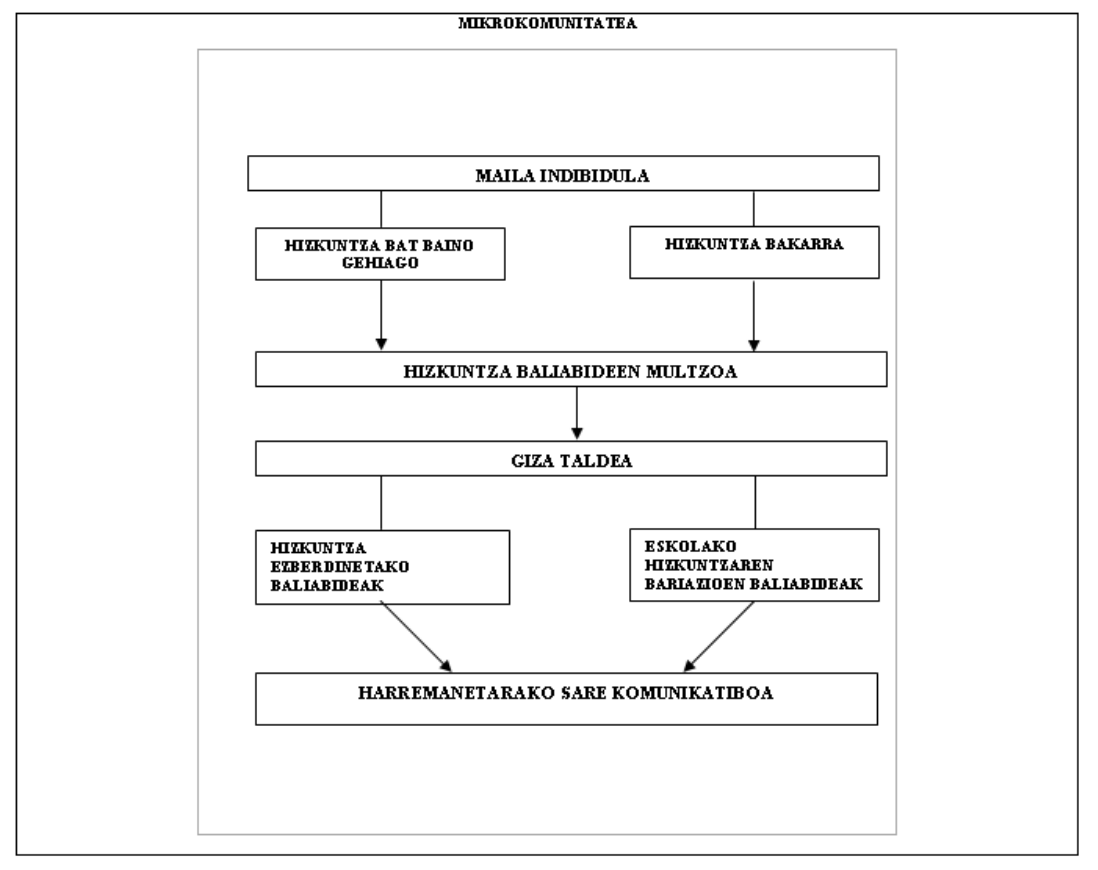
\includegraphics{assets/01_02-HD.png}

\hypertarget{metodoak}{%
\section{Metodoak}\label{metodoak}}

\textbf{Hizkuntza ulertzeko modua}-\textbf{Irakasteko modua}-\textbf{Metodologia ezberdinak}

\begin{itemize}
\tightlist
\item
  Gramatika/itzulpen metodoak
\item
  Eredu audiolinguala(egituren errepikapena, buruz ikasi)
\item
  Eredu kognoszitiboa (arauak)
\item
  Pragmatika eta eredu nozional/komunikaziozkoa:\emph{The communicative approach}
\end{itemize}

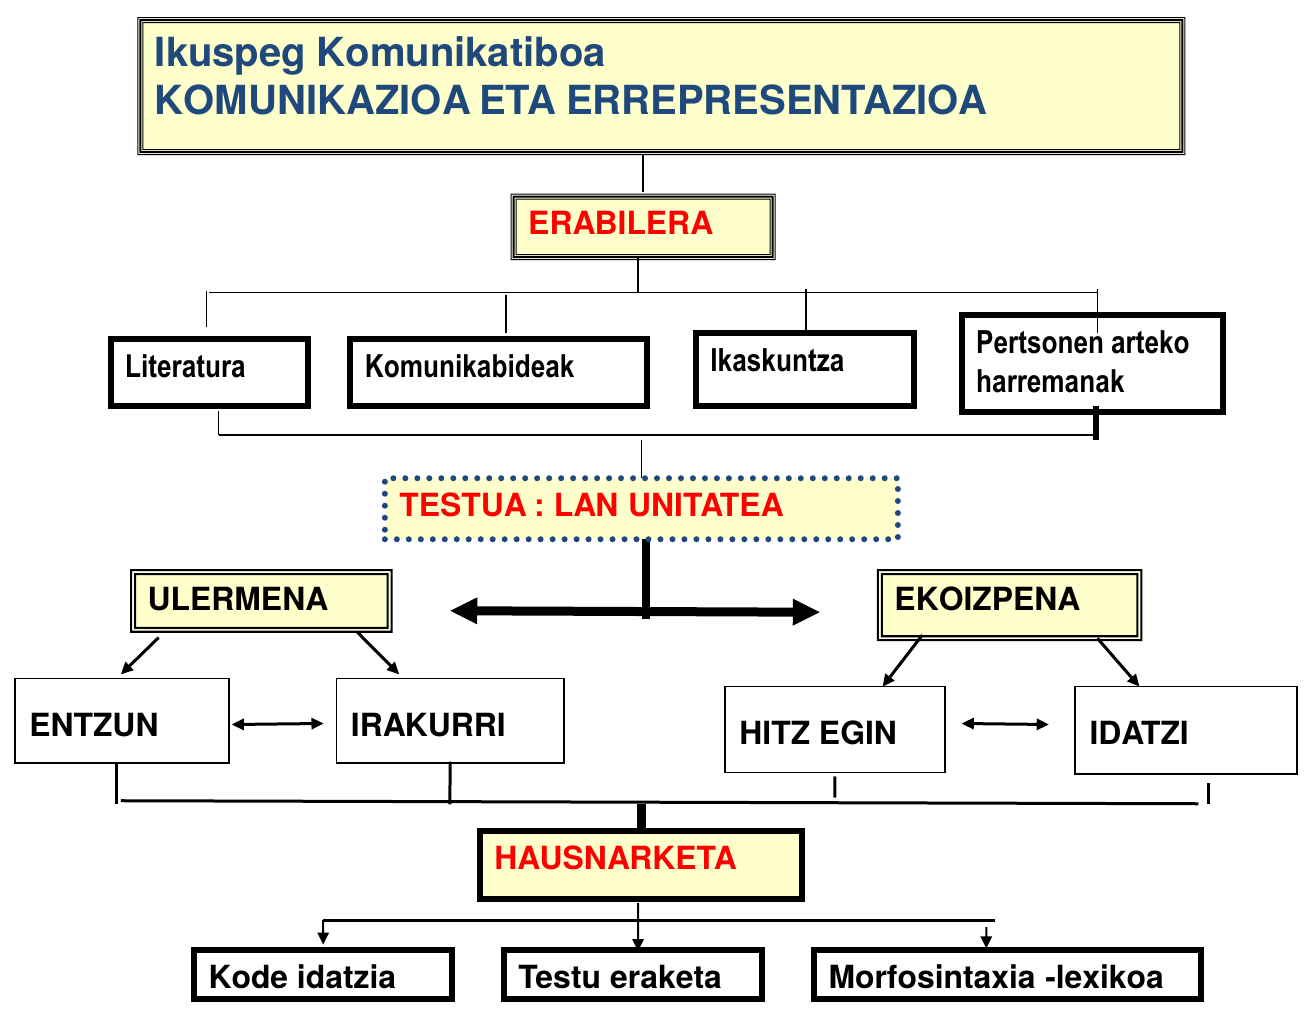
\includegraphics{assets/01_03-HD.png}

Testu horiek era egokian ``erabiltzea'' nahi badugu, gure lan eduki nagusiak trebezia mailakoak izango dira: hitz egiten, idazten, irakurtzen, entzuten irakastea izango da gure zeregina.
Eta testu horiek gero eta hobeto erabili ahal izateko, gero eta hobeto hitz egin, idatzi, irakurri edo entzuteko, egiten dugun horren inguruko hausnarketa beharko dugu. Gramatika eta hizkuntzaren sistemaren gaineko lanak beste era bateko funtzioa hartzen du, ez da aprendizaiaren helburu, baizik eta baliabide

\begin{center}\rule{0.5\linewidth}{0.5pt}\end{center}

\hypertarget{erreferentziak}{%
\section{Erreferentziak}\label{erreferentziak}}

Idiazabal I.(2003). Eskolaren kalitatea eta euskara.\emph{BAT Soziolinguistika Aldizkaria} 49, 2003, 195-199. ISSN: 1130-8435

Idiazabal, I., \& Manterola, I. (2009). Euskal eredu elebidunak, murgilketa eta hizkuntzen irakaskuntza bateratua: kontzeptuen berrikusketa. \emph{Euskera}, 54, 2--1. Eskuragarri \url{http://www.euskaltzaindia.net/dok/euskera/74632.pdf} helbidean

Lewis, M. P.(2005). Towards a categorization of endangerment of the world's languages.\_SIL International\_.

López Valero, A. (1998). Hacia una conformación histórica de la Didáctica de la Lengua y la Literatura. \emph{Didáctica. Lengua y literatura}, (10), 215--232.

Martí, F., Ortega, P., Idiazabal, I., Barreña, A., Juaristi, P., Junyent, C., \ldots{} Amorrortu, E.(2005).\emph{Hizkuntzen mundua. Munduko hizkuntzei buruzko txostena}. Bilbo: UPV/EHU.

Moseley, Christopher (ed.). \emph{2010. Atlas of the World's Languages in Danger}, 3rd edn. Paris:UNESCO Publishing. Online version: \url{http://www.unesco.org/culture/en/endangeredlanguages/atlas}

Moreno-Cabrera, J. C.(2008). \emph{El nacionalismo lingüístico: Una ideología destructiva}. Barcelona: Ediciones Península.

Sánchez, J. M.(1991). \emph{Un futuro para nuestro pasado. Claves de la recuperación del Euskara y teoría social de las lenguas} (Libk. 1). Donostia: Gipuzkoako Foru Aldundia. Berreskuratua \href{http://www.ehu.eus/ojs/index.php/ASJU/article/view/8593-\%28e\%29tik}{http://www.ehu.eus/ojs/index.php/ASJU/article/view/8593}-tik

\hypertarget{lehenengo-jarduera}{%
\chapter*{Lehenengo jarduera}\label{lehenengo-jarduera}}
\addcontentsline{toc}{chapter}{Lehenengo jarduera}

Landu Idiazabal \& Manterola (2008) testua, bertako kontzeptu gakoak ulertze aldera.

\hypertarget{taldearen-hizkuntz-esperientzia}{%
\subsection*{Taldearen hizkuntz esperientzia}\label{taldearen-hizkuntz-esperientzia}}
\addcontentsline{toc}{subsection}{Taldearen hizkuntz esperientzia}

Ikaskideen aurreko aurkezpena egin behar duzue aipatu testuko gako idiak kontuan izanda.

Honako kontzeptuok argitu behar dira irakurketaren bitartez, gero aurkezpenean egoki erabiltzeko.

\begin{itemize}
\tightlist
\item
  Ikasteredua
\item
  Eskola hizkuntza
\item
  Murgilketa eredua
\item
  D eredua
\item
  D eredu naturala
\item
  Tesuinguru euskalduna
\item
  Elebiduna
\item
  Elebakarra
\item
  Bigarren hizkuntza (H\textsubscript{2})
\item
  Garapen interdependentea
\end{itemize}

\begin{description}
\tightlist
\item[Lanerako galdera]
Zein izan da zuon taldearen eskarmentua hizkuntzaren ikaskuntzari dagokionez?
\end{description}

\hypertarget{hautazko-jarduera}{%
\section*{Hautazko jarduera:}\label{hautazko-jarduera}}
\addcontentsline{toc}{section}{Hautazko jarduera:}

\begin{itemize}
\tightlist
\item[$\square$]
  Irakurri \emph{Txepetx}ek\footnote{\emph{Txepetx} da Jose Maria Sánchezen desizena. izenpetu ere bere desizenez egiten zuenez, hori ere erabiltzeko ohitura zabaldu da.} dioena eta erantzun galderak. Horretarako aparteko laburpena dago, Telegrameko kanaleko lehenengotariko dokumentua edo \href{https://github.com/JuanAbasolo/HD/blob/01-gaia/1_Txepetx_testuak.pdf}{esteka honetan}.
\end{itemize}

\hypertarget{ahozko-aurkezpena-ebaluatzeko-errubrika}{%
\chapter*{Ahozko aurkezpena ebaluatzeko errubrika}\label{ahozko-aurkezpena-ebaluatzeko-errubrika}}
\addcontentsline{toc}{chapter}{Ahozko aurkezpena ebaluatzeko errubrika}

Hurrengo errubrika hau erabiliko dugu ahozko ebaluazioetarako

\begin{longtable}[]{@{}rllll@{}}
\toprule
\begin{minipage}[b]{0.11\columnwidth}\raggedleft
\strut
\end{minipage} & \begin{minipage}[b]{0.19\columnwidth}\raggedright
\textbf{Hobekuntza franko behar duen lana}\strut
\end{minipage} & \begin{minipage}[b]{0.19\columnwidth}\raggedright
\textbf{Lan nahikoa}\strut
\end{minipage} & \begin{minipage}[b]{0.19\columnwidth}\raggedright
\textbf{Lan ona}\strut
\end{minipage} & \begin{minipage}[b]{0.19\columnwidth}\raggedright
\textbf{Lan bikaina}\strut
\end{minipage}\tabularnewline
\midrule
\endhead
\begin{minipage}[t]{0.11\columnwidth}\raggedleft
\textbf{Taldeko lana}\strut
\end{minipage} & \begin{minipage}[t]{0.19\columnwidth}\raggedright
Taldekideen artean ez da elkarlanik egon eta lanean nabaritzen da\strut
\end{minipage} & \begin{minipage}[t]{0.19\columnwidth}\raggedright
Kohesio falta dago, lana taldekideen artean banatu dute baina oso zaila da tokatu zaien zatiaz hitz egitea.\strut
\end{minipage} & \begin{minipage}[t]{0.19\columnwidth}\raggedright
Lana taldekideen artean banatu dute baina azken entsegua denen artean egin dute.\strut
\end{minipage} & \begin{minipage}[t]{0.19\columnwidth}\raggedright
Koordinazio eta komunikazio handia dago, guztiek tokatu zaien zatia ondo egin dute.\strut
\end{minipage}\tabularnewline
\begin{minipage}[t]{0.11\columnwidth}\raggedleft
\textbf{Edukiak}\strut
\end{minipage} & \begin{minipage}[t]{0.19\columnwidth}\raggedright
Edukiak txarto hautau dituzte, txarto antolatuta daude eta errepikatuta\strut
\end{minipage} & \begin{minipage}[t]{0.19\columnwidth}\raggedright
Edukiak egokiak dira, baina edukiak hobeto antolatu daitezke\strut
\end{minipage} & \begin{minipage}[t]{0.19\columnwidth}\raggedright
Edukiak ondo aukeratu dituzte, ondo antolatuta daude eta ondo azalduta\strut
\end{minipage} & \begin{minipage}[t]{0.19\columnwidth}\raggedright
Edukiak ondo aukeratu dituzte, ondo antolatuta daude eta ondo azalduta.\strut
\end{minipage}\tabularnewline
\begin{minipage}[t]{0.11\columnwidth}\raggedleft
\textbf{Irudia}\strut
\end{minipage} & \begin{minipage}[t]{0.19\columnwidth}\raggedright
Kolorea txarto aukeratu da, testu gehiegi, ikusteko arazoak.\strut
\end{minipage} & \begin{minipage}[t]{0.19\columnwidth}\raggedright
Aurkezpena ondo ikusten da, baina itxusia da.\strut
\end{minipage} & \begin{minipage}[t]{0.19\columnwidth}\raggedright
Argazkiak ondo aukeratu dira, testua orekatua da, ondo ikusten da.\strut
\end{minipage} & \begin{minipage}[t]{0.19\columnwidth}\raggedright
Argazkiak ondo aukeratu dira, testua orekatua da, gainera, ikusten dena oso erakargarria da.\strut
\end{minipage}\tabularnewline
\begin{minipage}[t]{0.11\columnwidth}\raggedleft
\textbf{Ahozko aurkezpena}\strut
\end{minipage} & \begin{minipage}[t]{0.19\columnwidth}\raggedright
Isilune handiak, testua falta da. Diapositibak nahasten dira.\strut
\end{minipage} & \begin{minipage}[t]{0.19\columnwidth}\raggedright
Aurkezpena egokia da, baina denboretara egokitzeko arazoak. Ahozkera arazoak.\strut
\end{minipage} & \begin{minipage}[t]{0.19\columnwidth}\raggedright
Aurkezpen egokia, denboretara ondo egokituta, ahozkera ona.\strut
\end{minipage} & \begin{minipage}[t]{0.19\columnwidth}\raggedright
Aurkezpen egokia, denboretara ondo egokituta, ahozkera ona. Gorpuzkerak, aurpegikerak eta keinuek diskurtsoari indarra ematen diote.\textbar{}\strut
\end{minipage}\tabularnewline
\bottomrule
\end{longtable}

\hypertarget{hizkuntza-eta-ageriko-curriculuma}{%
\chapter{Hizkuntza eta ageriko curriculuma}\label{hizkuntza-eta-ageriko-curriculuma}}

\href{https://gitpitch.com/JuanAbasolo/HD/02-gaia?grs=github\&t=moon}{
\includegraphics{assets/badge.png}}

Hizkuntza eskolan tratatzeko erez ari garenean, kontuan izan behar dugu horren inguruan ereikitako lege ikuspegi osoa. Besteak beste, horren arabera sortu beharko duzuelako dena delako elementua oposizioak-eta egiteko.

Curriculumez ari garenean hitz egin dezakegu eskola esperientziak eragindako bizipen/ikaskuntzez edota aurrez prestatutako ikaskuntza-ibilbiderako planez. Oraingo honetan bigarren horri buruz hausnartu behar dugu: Curriculum diseinuaz.

Legeen bitartez eraikitzen da curriculumaren lehenengo zehaztapen maila. Kapitulu honetan legeei begiratu behar diegu, zehazki, hizkuntzari begiratzen dion alderdia landuko dugu.

Lege markoa matroysken antzera eregiten da, pausu bakoitzak jarraikortasuna behar du aurrekoarekiko. Euskal Herriko ikasgeletara iristen den legearen forma aurretiko beste lege batzuk moldatutakoa da.

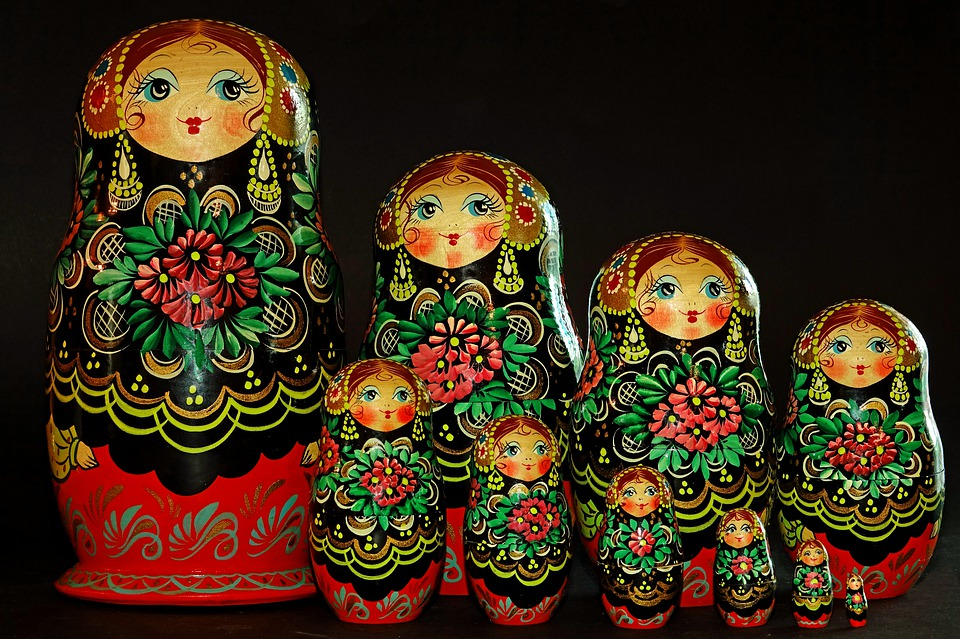
\includegraphics{assets/ornament-3131097_960_720.jpg}
\href{https://pixabay.com/en/ornament-matryoshka-babuschka-3131097/}{iturria}

Gure kasuan, UPV/EHUk baskongadetako errealitateari begiratu behar dionez, Heziberri 2020 planak ezartzen duen errealitatea aztertuko dugu. Baina Euskal Herriko ikuspegi zabalago batetik ere begira genezaioke Ipar Euskal Herriko lege markoa edota Nafarroakora egokituta, dagozkien elementuak.

Gaur egungo paradigmatik ulertuta, hezkuntzaz aritzeak esan nahi du gaikuntzaz hitz egitea, gaitasunak garatzeari buruz jardutea.

Horrela, gaurko lege-markoa ulertzeko paradigamren eraikuntzatik hasi, legeek egiten duten interpretaziora pasa eta gelako jardunaren diseinura iritsi behar dugu. Matryoskak bailiran legez

\begin{itemize}
\tightlist
\item
  Delors txostena (UNESCO) 1998\\
  Education for the twenty-first century: issues and prospects: contributions to the work of the International Commission on Education for the Twenty-First Century (\href{http://unesdoc.unesco.org/images/0011/001147/114766e.pdf}{en})\\
  La educación encierra un tesoro (\href{http://www.unesco.org/education/pdf/DELORS_S.PDF}{es})
\item
  DeSeCo (OCDE)
  Definition and Selection of Competences (DeSeCo): Theoretical and conceptual foundations (2002)\href{http://deseco.ch/bfs/deseco/en/index/02.parsys.34116.downloadList.87902.DownloadFile.tmp/oecddesecostrategypaperdeelsaedcericd20029.pdf}{(*)}
  Key Competencies for a Successful Life and a Well-Functioning Society (2003)
  Definition and Selection of Key Competencies - Executive Summary\href{http://deseco.ch/bfs/deseco/en/index/02.parsys.43469.downloadList.2296.DownloadFile.tmp/2005.dskcexecutivesummary.en.pdf}{*} (2005)
\item
  Gaitasun giltzarriak (Europar Legebiltzarra)
  \href{http://eur-lex.europa.eu/legal-content/EN/TXT/?uri=CELEX:32006H0962}{2006/962/CE} (\href{http://infofpe.cea.es/fpe/norm/Rec\%2018_2006.pdf}{es})
  Recommendation of the European Parliament and of the Council of 18 December 2006 on key competences for lifelong learning.
\item
  LOMCE 8/2013 + Frantziako ordenamendua
\item
  Curriculuma 126/2014 + Frantziako Curriculuma
\item
  Agindua ECD/65/2015 + Frantziako baliokidea
\item
  Oinarrizko Hezkuntzarako curriculum Dekretua + Nafarroako ordenamendua
\end{itemize}

\begin{center}\rule{0.5\linewidth}{0.5pt}\end{center}

\hypertarget{hegoaldeko-lege-markoa}{%
\section{Hegoaldeko lege markoa}\label{hegoaldeko-lege-markoa}}

Hemen Hegoaldeko kasuaren azterketan ardazten ari gara analisia, baina berdin egin liteke Iparraldeari begiratu nahi bageuntse Frantziako kasua aztertuaz. Hori ikusteko, \href{http://www.vc.ehu.es/araka/orri12.htm}{Araka}ko web orriko baliabideak interesgarriak izan daitezke, baina kontuan izan behar da azken legeak ez dituela hartzen.

\hypertarget{lomce}{%
\subsection{LOMCE}\label{lomce}}

Ley Orgánica 8/2013, de 9 de diciembre, para la mejora de la calidad educativa\href{https://www.boe.es/buscar/act.php?id=BOE-A-2013-12886}{*}.

\begin{quote}
\ldots{} Obligatoria en un curso fundamentalmente propedéutico y con dos trayectorias bien diferenciadas.

La LOMCE hace especial incidencia con vistas a la transformación del sistema educativo: las Tecnologías de la Información y la Comunicación, el fomento del plurilingüismo, y la modernización de la Formación Profesional.
\end{quote}

\hypertarget{curriculuma-ezartzeko-dekretua}{%
\subsection{Curriculuma ezartzeko dekretua}\label{curriculuma-ezartzeko-dekretua}}

126/2014 Erret dekretua\href{https://www.boe.es/buscar/pdf/2014/BOE-A-2014-2222-consolidado.pdf}{*}

Real Decreto 126/2014, de 28 de febrero, por el que se establece el currículo básico de la Educación Primaria\href{https://www.boe.es/buscar/pdf/2014/BOE-A-2014-2222-consolidado.pdf}{*}.

\begin{quote}
\ldots se entiende por currículo la regulación de los elementos que determinan los procesos de enseñanza y aprendizaje para cada una de las enseñanzas\ldots{}
\end{quote}

Ikasgaien antolaketa ere dekretu horretan zehazten da:

\begin{itemize}
\tightlist
\item
  Curriculuma
\item
  Helburuak
\item
  Konpetentziak
\item
  Edukiak
\item
  Ikaskuntza estandarrak
\item
  Ebaluazio irizpideak
\item
  Metodologia didaktikoa
\end{itemize}

\hypertarget{gaitasunak-edukiak-eta-ebaluazio-irizpideak}{%
\subsection{Gaitasunak, edukiak eta ebaluazio irizpideak}\label{gaitasunak-edukiak-eta-ebaluazio-irizpideak}}

Zehazten dira ECD/65/2015 Aginduan\href{https://www.boe.es/buscar/doc.php?id=BOE-A-2015-738}{*}

Orden ECD/65/2015, de 21 de enero, por la que se describen las relaciones entre las competencias, los contenidos y los criterios de evaluación de la educación primaria, la educación secundaria obligatoria y el bachillerato

\hypertarget{honako-konpetentziak-zehazten-dira}{%
\subsubsection{Honako konpetentziak zehazten dira:}\label{honako-konpetentziak-zehazten-dira}}

\begin{enumerate}
\def\labelenumi{\arabic{enumi}.}
\tightlist
\item
  Comunicación lingüística.
\item
  Competencia matemática y competencias básicas en ciencia y tecnología.
\item
  Competencia digital.
\item
  Aprender a aprender.
\item
  Competencias sociales y cívicas.
\item
  Sentido de iniciativa y espíritu emprendedor.
\item
  Conciencia y expresiones culturales.
\end{enumerate}

\hypertarget{legedia-hizkuntzaren-didaktikaren-arautzailea}{%
\subsection{Legedia, hizkuntzaren didaktikaren arautzailea}\label{legedia-hizkuntzaren-didaktikaren-arautzailea}}

\begin{longtable}[]{@{}rccccc@{}}
\toprule
\begin{minipage}[b]{0.11\columnwidth}\raggedleft
\strut
\end{minipage} & \begin{minipage}[b]{0.14\columnwidth}\centering
Ebaluazioa\strut
\end{minipage} & \begin{minipage}[b]{0.14\columnwidth}\centering
Hizkuntza ofizial eta koofizialak\strut
\end{minipage} & \begin{minipage}[b]{0.14\columnwidth}\centering
Atzerriko hizkuntza\strut
\end{minipage} & \begin{minipage}[b]{0.14\columnwidth}\centering
Komunikazio gaitasuna\strut
\end{minipage} & \begin{minipage}[b]{0.14\columnwidth}\centering
Ikuspuntu komunikatiboa\strut
\end{minipage}\tabularnewline
\midrule
\endhead
\begin{minipage}[t]{0.11\columnwidth}\raggedleft
\textbf{LOMCE}\strut
\end{minipage} & \begin{minipage}[t]{0.14\columnwidth}\centering
x\strut
\end{minipage} & \begin{minipage}[t]{0.14\columnwidth}\centering
\strut
\end{minipage} & \begin{minipage}[t]{0.14\columnwidth}\centering
\strut
\end{minipage} & \begin{minipage}[t]{0.14\columnwidth}\centering
\strut
\end{minipage} & \begin{minipage}[t]{0.14\columnwidth}\centering
\strut
\end{minipage}\tabularnewline
\begin{minipage}[t]{0.11\columnwidth}\raggedleft
\textbf{Curriculum Dekretua}\strut
\end{minipage} & \begin{minipage}[t]{0.14\columnwidth}\centering
x\strut
\end{minipage} & \begin{minipage}[t]{0.14\columnwidth}\centering
x\strut
\end{minipage} & \begin{minipage}[t]{0.14\columnwidth}\centering
x\strut
\end{minipage} & \begin{minipage}[t]{0.14\columnwidth}\centering
x\strut
\end{minipage} & \begin{minipage}[t]{0.14\columnwidth}\centering
\strut
\end{minipage}\tabularnewline
\begin{minipage}[t]{0.11\columnwidth}\raggedleft
\textbf{ECD 65/2015 Agindua}\strut
\end{minipage} & \begin{minipage}[t]{0.14\columnwidth}\centering
\strut
\end{minipage} & \begin{minipage}[t]{0.14\columnwidth}\centering
\strut
\end{minipage} & \begin{minipage}[t]{0.14\columnwidth}\centering
\strut
\end{minipage} & \begin{minipage}[t]{0.14\columnwidth}\centering
x\strut
\end{minipage} & \begin{minipage}[t]{0.14\columnwidth}\centering
\strut
\end{minipage}\tabularnewline
\begin{minipage}[t]{0.11\columnwidth}\raggedleft
\textbf{Heziberri 2020}\strut
\end{minipage} & \begin{minipage}[t]{0.14\columnwidth}\centering
x\strut
\end{minipage} & \begin{minipage}[t]{0.14\columnwidth}\centering
x\strut
\end{minipage} & \begin{minipage}[t]{0.14\columnwidth}\centering
x\strut
\end{minipage} & \begin{minipage}[t]{0.14\columnwidth}\centering
x\strut
\end{minipage} & \begin{minipage}[t]{0.14\columnwidth}\centering
x\strut
\end{minipage}\tabularnewline
\bottomrule
\end{longtable}

\hypertarget{oinarrizko-konpetentzia-giltzei-buruzko-proposamen-arteko-erlazioa}{%
\section{\texorpdfstring{Oinarrizko konpetentzia giltzei buruzko proposamen arteko erlazioa \href{http://www.hezkuntza.ejgv.euskadi.eus/contenidos/informacion/heziberri_2020/eu_erlazioa/adjuntos/oinarrizko_konpetentzia_giltzei_buruzko_proposamen_arteko_erlazioa.pdf}{*}}{Oinarrizko konpetentzia giltzei buruzko proposamen arteko erlazioa *}}\label{oinarrizko-konpetentzia-giltzei-buruzko-proposamen-arteko-erlazioa}}

\begin{figure}
\centering
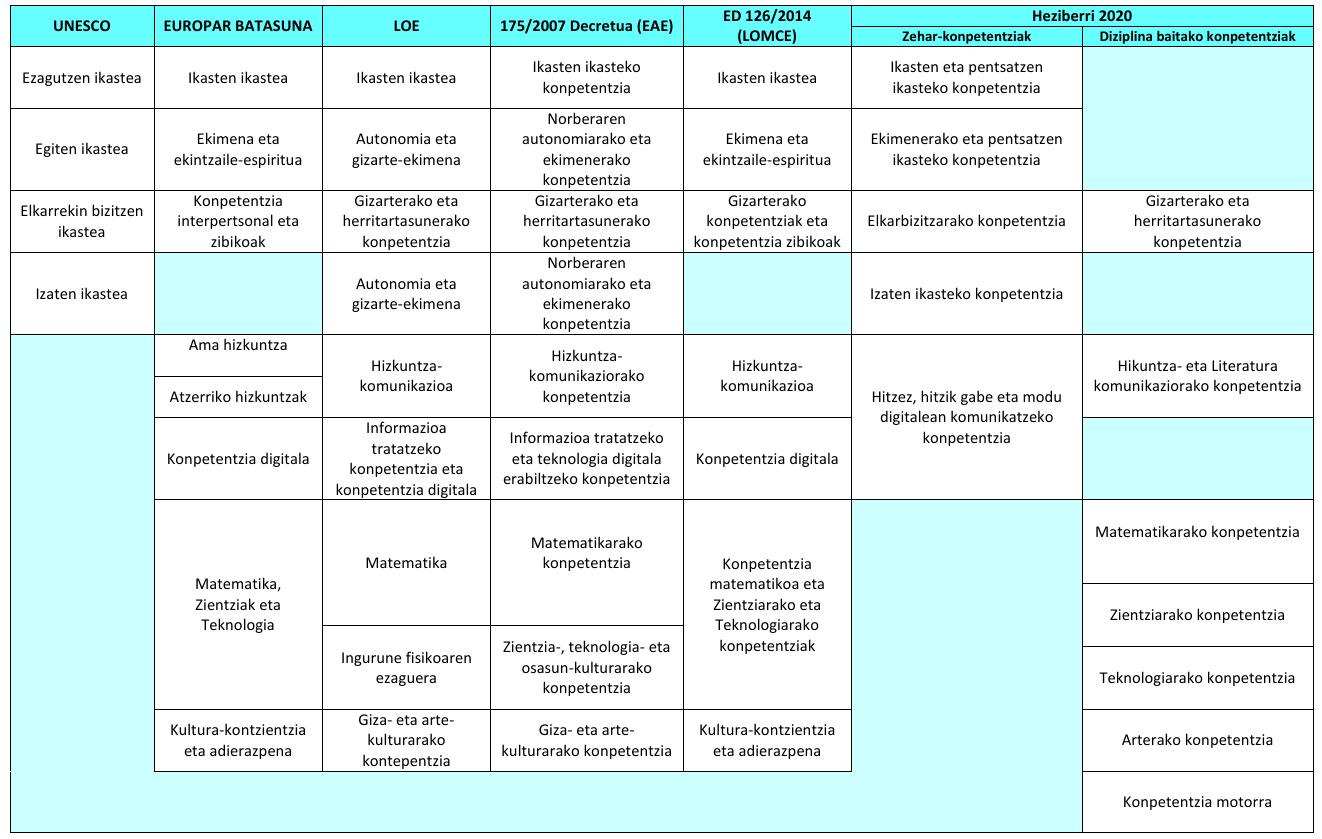
\includegraphics{assets/02_01-HD.png}
\caption{EJ}
\end{figure}

\hypertarget{baskongadeei-dagokien-araudia}{%
\section{Baskongadeei dagokien araudia}\label{baskongadeei-dagokien-araudia}}

Kontuan izan dezagun, soilik Euskal Autonomia Elkarteaz ari bagara, ez dugula kontuan hartzen Hegoaldeko hezkuntza errealitatea. Ber analisia egin dakioke Nafar curriculumari zein besteren bati ere.

\hypertarget{oinarrizko-hezkuntzarako-curriculum-dekretua}{%
\subsection{\texorpdfstring{Oinarrizko Hezkuntzarako curriculum dekretua \href{https://www.euskadi.eus/y22-bopv/eu/bopv2/datos/2016/01/1600141e.shtml}{*}}{Oinarrizko Hezkuntzarako curriculum dekretua *}}\label{oinarrizko-hezkuntzarako-curriculum-dekretua}}

\href{http://www.jusap.ejgv.euskadi.eus/r47-bopvapps/es/bopv2/datos/2016/01/1600141e.pdf}{236/2015 Dekretua}, abenduaren 22koa, Oinarrizko Hezkuntzaren curriculuma zehaztu eta Euskal Autonomia Erkidegoan ezartzen duena (EHAA, 2016-01-15)

\hypertarget{hizkuntza--eta-literatura--komunikaziorako-konpetentzia.}{%
\subsubsection{1. Hizkuntza- eta literatura- komunikaziorako konpetentzia.}\label{hizkuntza--eta-literatura--komunikaziorako-konpetentzia.}}

1.1.2.-- Eduki multzoen ezaugarriak.

Lehen Hezkuntzari dagozkion adierazpenezko, prozedurazko eta jarrerazko edukiak honako eduki multzo hauetan multzokatzen dira:

\hypertarget{eduki-multzoak}{%
\subsubsection{Eduki multzoak}\label{eduki-multzoak}}

\begin{enumerate}
\def\labelenumi{\arabic{enumi}.}
\tightlist
\item
  Arlo guztietan komunak diren oinarrizko zehar-konpetentziekin lotutako edukiak.
\item
  Ahozko komunikazioa: hitz egitea, entzutea eta elkarrekin solasean jardutea.
\item
  Idatzizko komunikazioa: irakurtzea eta idaztea.
\item
  Literatura-hezkuntza.
\item
  Hizkuntzari eta haren erabilerei buruzko gogoeta.
\item
  Hizkuntzaren alderdi soziala.
\end{enumerate}

\begin{center}\rule{0.5\linewidth}{0.5pt}\end{center}

\hypertarget{kapituluko-erreferentziak}{%
\section{Kapituluko erreferentziak}\label{kapituluko-erreferentziak}}

Araka ikertaldea. (2003). Araka ikertaldea - legeria \[web\]. Berreskuratua 2018(e)ko otsailakaren 9a, \url{http://www.vc.ehu.es/araka/orri12.htm} etik

Centro Universitario de Desarrollo Intelectual. (2016). Catálogo de rúbricas para la evaluación del aprendizaje. Berreskuratua \href{http://evirtual.uaslp.mx/FCQ/estrategias/Material\%20de\%20Apoyo/cat_rubrica.pdf}{http://evirtual.uaslp.mx/FCQ/estrategias/Material de Apoyo/cat\_rubrica.pdf} -etik

Delors, J., International Commission on Education for the Twenty-First Century, \& UNESCO (Arg.). (1998). \emph{Education for the twenty-first century: issues and prospects: contributions to the work of the International Commission on Education for the Twenty-First Century}. Paris: UNESCO Publishing.

EURIDYCE (Arg.). (2002). \emph{Key competencies: a developing concept in general compulsory education}. Brussels.

Europar Batasuna. (2006). \emph{2006/962/CE Recommendation of the European Parliament and of the Council of 18 December 2006 on key competences for lifelong learning} (Gomendioa No.~32006H0962) (or. 10\textasciitilde18). Estrasburgo: Europako Parlamentua. Berreskuratua \url{http://data.europa.eu/eli/reco/2006/962/oj/eng} -etik

EURYDICE. (2003). \emph{Las Competencias clave: un concepto en expansión dentro de la educación general obligatoria.} Madril: Eurydice. Unidad Española. Berreskuratua \url{http://www.hezkuntza.ejgv.euskadi.eus/contenidos/informacion/dig_publicaciones_innovacion/es_curricul/adjuntos/14_curriculum_competencias_300/300001c_Pub_UE_Eurydice_Competencias_c.pdf} -etik

Eusko Jaurlaritza (Hezkuntza, Hizkuntza Politika eta Kultura Saila). (2017). Oinarrizko konpetentzia giltzei buruzko proposamen arteko erlazioa \[pdf formatudun dokumentoa\]. Berreskuratua 2018(e)ko otsailakaren 9a, \url{http://www.hezkuntza.ejgv.euskadi.eus/contenidos/informacion/heziberri_2020/eu_erlazioa/adjuntos/oinarrizko_konpetentzia_giltzei_buruzko_proposamen_arteko_erlazioa.pdf} -etik

Eusko Jaurlaritzaren legebiltzarra. (2015). 236/2015 Dekretua, abenduaren 22koa, Oinarrizko Hezkuntzaren curriculuma zehaztu eta Euskal Autonomia Erkidegoan ezartzen duena. \emph{Euskal Herriko Agintaritzaren Aldizkaria, 2016ko urtarrilaren 15a}, \emph{141}. Berreskuratua \url{https://www.euskadi.eus/y22-bopv/eu/bopv2/datos/2016/01/1600141e.shtml} -etik

Gobierno de España. (2013). Ley Orgánica 8/2013, de 9 de diciembre, para la mejora de la calidad educativa. \emph{Boletín Oficial del Estado}. Berreskuratua \url{https://www.boe.es/buscar/act.php?id=BOE-A-2013-12886} -tik

Gobierno de España (Ministerio de Educación, Cultura y Deporte). (2014). Real Decreto 126/2014, de 28 de febrero, por el que se establece el currículo básico de la Educación Primaria. \emph{Boletín Oficial del Estado}, \emph{52}, 19349--19420. Berresekuratua \url{https://www.boe.es/buscar/act.php?id=BOE-A-2014-2222} -tik

Gobierno de España (Ministerio de Educación, Cultura y Deporte). (2015). Orden Ecd/65/2015, de 21 de enero, por la que se describen las relaciones entre las competencias, los contenidos y los criterios de evaluación de la educación primaria, la educación secundaria obligatoria y el bachillerato. \emph{Boletín Oficial de Estado}, (25). Berreskuratua \url{https://www.boe.es/buscar/doc.php?id=BOE-A-2015-738} -tik

Organisation for Economic Co-operation and Development. (2002, urriak 7). Definition and Selection of Competences (DeSeCo): Theoretical and conceptual foundations. Berreskuratua \url{http://deseco.ch/bfs/deseco/en/index/02.parsys.34116.downloadList.87902.DownloadFile.tmp/oecddesecostrategypaperdeelsaedcericd20029.pdf} -etik

Organisation for Economic Co-operation, \& Development (OECD). (2005). \emph{The definition and selection of key competencies: Executive summary}. OECD Paris. Berreskuratua \url{http://deseco.ch/bfs/deseco/en/index/02.html} -etik

Organización para la Cooperación y el Desarrollo Económicos (OCDE). (2015). \emph{La definición selección de las competencias clave. Resumen ejecutivo}.

Rychen, D. S., \& Salganik, L. H. (Arg.). (2003). \emph{Key competencies for a successful life and a well-functioning society}. Cambridge, Massachusetts: Hogrefe \& Huber.

\hypertarget{bigarren-jarduera}{%
\chapter*{Bigarren jarduera}\label{bigarren-jarduera}}
\addcontentsline{toc}{chapter}{Bigarren jarduera}

\begin{itemize}
\item
  Oinarrizko Hezkuntzako Curriculuma
  (236/2015eko Dekretuaren II. Eranskina osatzen duen curriculum orientatzailea)
\item
  Aurkeztu eta konpartitu:
  Sort ezazu egokitu zaizuen multzoaren eskema. Ikaskideei aurkeztu eta eurekin partekatu beharko duzue.
\end{itemize}

\textbf{Ebaluazioa} egiteko \href{http://evirtual.uaslp.mx/FCQ/estrategias/Material\%20de\%20Apoyo/cat_rubrica.pdf}{hau} erabiliko dut.

\hypertarget{ahozko-trebetasuna-lhn}{%
\chapter{Ahozko Trebetasuna LHn}\label{ahozko-trebetasuna-lhn}}

\href{../Diapoak/03_Diap-ahozko_trebetasunak.html}{
\includegraphics{assets/badge.png}}

Hizkuntzen irakaskuntzan ikuspegi eta metodo ezberdinak eraman dira
praktikara eta ahozko komunikazioak ez du beti toki bera izan:

\begin{longtable}[]{@{}lll@{}}
\caption{Metodoen garapenaz}\tabularnewline
\toprule
\begin{minipage}[b]{0.21\columnwidth}\raggedright
\strut
\end{minipage} & \begin{minipage}[b]{0.35\columnwidth}\raggedright
Ikuspegia/Metodoa\strut
\end{minipage} & \begin{minipage}[b]{0.35\columnwidth}\raggedright
Ahozkotasunarenirakaskuntza\strut
\end{minipage}\tabularnewline
\midrule
\endfirsthead
\toprule
\begin{minipage}[b]{0.21\columnwidth}\raggedright
\strut
\end{minipage} & \begin{minipage}[b]{0.35\columnwidth}\raggedright
Ikuspegia/Metodoa\strut
\end{minipage} & \begin{minipage}[b]{0.35\columnwidth}\raggedright
Ahozkotasunarenirakaskuntza\strut
\end{minipage}\tabularnewline
\midrule
\endhead
\begin{minipage}[t]{0.21\columnwidth}\raggedright
XX. Mendearen aurretik\strut
\end{minipage} & \begin{minipage}[t]{0.35\columnwidth}\raggedright
Metodo zuzena edo Naturala\strut
\end{minipage} & \begin{minipage}[t]{0.35\columnwidth}\raggedright
Ahozko elkarreragina:irakaslearen galdera-ikaslearen erantzuna\strut
\end{minipage}\tabularnewline
\begin{minipage}[t]{0.21\columnwidth}\raggedright
XX. mendea\strut
\end{minipage} & \begin{minipage}[t]{0.35\columnwidth}\raggedright
Metodo Estrukturalistak:Situaliazionala eta Audiolinguala\strut
\end{minipage} & \begin{minipage}[t]{0.35\columnwidth}\raggedright
Egituren errepikapenaDena ahoz lantzen da eta idatzizko hizkuntza bigarren maila\strut
\end{minipage}\tabularnewline
\begin{minipage}[t]{0.21\columnwidth}\raggedright
Ikuspegi eta metodo alternatiboak\strut
\end{minipage} & \begin{minipage}[t]{0.35\columnwidth}\raggedright
Erantzun fisiko Totala, Metodo Isila,Hizkuntzaren Ikaskuntza Komunitarioa,Sugestopedia,Adimen anitzak,Ikuspegi Lexikoaeta Gaitasunetan Oinarritutako Hizkuntzen Irakaskuntza.\strut
\end{minipage} & \begin{minipage}[t]{0.35\columnwidth}\raggedright
Gramatikaren irakaspenari emandako garrantzitik alde egin nahi zuten, eta ikasgeletan elkarrizketarako tartea zabaldu.\strut
\end{minipage}\tabularnewline
\begin{minipage}[t]{0.21\columnwidth}\raggedright
Gaur egungo ikuspegi komunikatiboak\strut
\end{minipage} & \begin{minipage}[t]{0.35\columnwidth}\raggedright
Hizkuntzaren Irakaskuntza Komunikatiboa,Ikuspegi Naturala,Hizkuntzaren Ikaskuntza Kooperatiboa,Edukietan Oinarritutako Instrukzioa,Atazetan Oinarritutako Hizkuntzaren Irakaskuntza eta post-metodo aroa.\strut
\end{minipage} & \begin{minipage}[t]{0.35\columnwidth}\raggedright
Ikasleen arteko harremanak sortzea; ez bakarrik egiturak ezagutzea.Ikasleek hizkuntza ikasiko dute komunikatzeko beharragatik\strut
\end{minipage}\tabularnewline
\bottomrule
\end{longtable}

\hypertarget{ahozko-ekoizpen-eta-jarduera-motak}{%
\section{Ahozko ekoizpen eta jarduera motak}\label{ahozko-ekoizpen-eta-jarduera-motak}}

\begin{itemize}
\tightlist
\item
  Adierazpen publikoak egitea (informazioa, jarraibideak, etab.)
\item
  Jendaurrean hitz egitea (azalpenak ematea bileretan, unibertsitateko hitzaldiak, sermoiak, ikuskizunak, kiroletako azalpenak, salmenten aurkezpenak, etab.)
\item
  Elkarrizketak
\end{itemize}

\ldots eta ekintza horiek hurrengoak eska ditzakete:

\begin{itemize}
\tightlist
\item
  Idatzizko testu bat ozen irakurtzea;
\item
  Oharretan, idatzizko testu batean edo ikusizko elementuetan (eskemak, irudiak,
  grafikoak, etab.) oinarrituta hitz egitea;
\item
  Aldez aurretik prestatutako zerbait antzeztea;
\item
  Bat-batean hitz egitea;
\item
  Abestea.
\end{itemize}

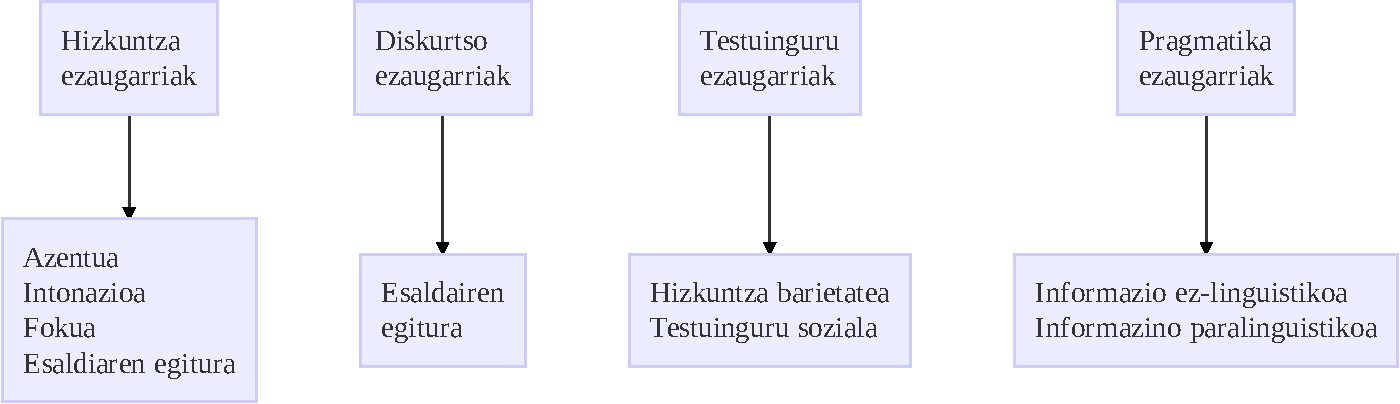
\includegraphics{bookdown-demo_files/figure-latex/unnamed-chunk-2-1.pdf}

\hypertarget{bazter-utzitako-eremua}{%
\section{Bazter utzitako eremua}\label{bazter-utzitako-eremua}}

\begin{quote}
Hizkuntzaren ikaskuntzan nahiz irakaskuntzan, sarritan, ahozkotasuna ahaztu
egin da. Horren ondorioz, ahozkotasunaren ezaugarri segmentalak
(kontsonanteak eta bokalak) nahiz suprasegmentalak (erritmoa, azentua eta
intonazioa) sarritan ez omen ditugu irakatsi

---\emph{Usó, 2008}
\end{quote}

\begin{quote}
El papel marginal de la pronunciación tanto en
los materiales didácticos (en la introducción, en
el apéndice, en actividades desligadas del tema
de la unidad\ldots{} ) como en las publicaciones en
el ámbito de la didáctica de la LE.

---\emph{Cortés Moreno, 2001: 128}
\end{quote}

\hypertarget{garrantziaz}{%
\subsection{Garrantziaz}\label{garrantziaz}}

\begin{quote}
Hoy en día, muchos profesionales sin conocimientos específicos de fonética
quieren o necesitan por motivos laborales adaptar su pronunciación al uso
estándar de la lengua y alejar, en su proyección pública, rasgos considerados
demasiado dialectales o marcados especialmente de algún modo. Pueden estar
en este caso periodistas, locutores de televisión y de radio, cantantes de éxito,
políticos, empresarios, financieros\ldots{} Para dirigirse a un amplio público y
transmitir mensajes alejados de la broma como puede ser un telediario o un
discurso de política general puede ser interesante intentar circunscribirse a un
estilo estándar formal de pronunciación para que aspectos marcadamente
dialectales o sociales no desvíen la atención del contenido que se pretende
transmitir. También puede verse en esta situación un actor o una actriz que para
poder trabajar deba disimular su acento original o, por el contrario, deba
adoptar un acento que no es el suyo nativo.

---\emph{Fernández, 2007:43}
\end{quote}

\hypertarget{baliabideak}{%
\subsection{Baliabideak}\label{baliabideak}}

BIDEOJOKOAK: Bideojokoak sortu izan dira behar bereziak dituztenei
laguntzeko (Corrales, 2015; Aguilar et. al., 2015), izan ere bideojokoek aukera
ematen dute errealiatea errepresentatzeko, hiztunen arteko erlazioak
adierazteko eta komunikazio egoeretan gertatzen diren kausa-ondorio erlazioak
lantzeko (Aguilar et. al., 2015).

\hypertarget{pradia-bideojokoa}{%
\subsubsection{\texorpdfstring{\href{http://pradia.net/}{Pradia} bideojokoa:}{Pradia bideojokoa:}}\label{pradia-bideojokoa}}

Intonazio eta emozio patroiak
Identifikatu eta lantzeko.
Batez ere behar bereziak dituzten
Umeentzako baliabidea da.

\hypertarget{jolasak}{%
\subsubsection{Jolasak}\label{jolasak}}

Hurrengoa Gaminde eta beste (2014) liburutik hartutako adibidea duzu

\begin{quote}
\textbf{ESKU JOLASA}

\textbf{Antolaketa}: Binaka.

\textbf{Helburua}: Emozioen adierazpena lantzea.

\textbf{Materiala}: Errezitatu bat.

\textbf{Prozesua}: Jolasarekin hasi aurretik: Irakasleak binaka jarriko ditu umeak
eta errezitatu bitartean zati batzuk pozik, haserre eta triste adieraziko
dituztela esango die, irakasleak aukeratuko du zer zati esango duten
pozik, haserre ala triste, eta emozio mota adierazten dutenean, ikasleek
era horretan errezitatuko dute.
Jolasaren hasieran: Errezitatu hau denen artean esango dute ahoz
gora:

\emph{Arre arre mandako\\
Bihar Tolosarako\\
Etzi Iruñerako\\
Handik zer ekarriko\\
Zapata ta gerriko}\\
---Gaminde, 2007

\emph{Jolastu bitartean}: Eskuekin binaka jolastuko dira, errezitatu bitartean
binaka ezkuekin jolastuko dira eta irakasleak emozio mota adieraztean
errezitatua adierazteko era emozio horretarako moldatuko dute.

---\emph{Gaminde et al.~2014}
\end{quote}

\hypertarget{trebetasunak-eta-sekuentzia-didaktikoak}{%
\section{Trebetasunak eta sekuentzia didaktikoak}\label{trebetasunak-eta-sekuentzia-didaktikoak}}

\begin{itemize}
\tightlist
\item
  ikasgela txokoetan antolatzen da
\item
  antolatzeko era ezberdinak: espazio eta denbora berean
\item
  bakarkako zein taldekako ariketa ezberdinak landu daitezke aldi berean
\item
  ikasleak autonomiaz aritzen dira
\item
  irakasle zein ikaskideei laguntza eskatzeko aukera dago
\item
  irakasleak ikasleak behatzeko aukera zabalagoa du
\end{itemize}

\hypertarget{hirugarren-jarduera-13}{%
\chapter*{Hirugarren jarduera (1/3)}\label{hirugarren-jarduera-13}}
\addcontentsline{toc}{chapter}{Hirugarren jarduera (1/3)}

\href{http://heziberri.berritzegunenagusia.eus/heziberri_eus/}{Heziberri 2020} proiektuaren barruan badira zenbait \emph{sekuentzia didaktiko}. Hortik hasita nabigatu behar duzu sekuentzia didaktiko batzuk aurkitzeko; aurkitutakoan txosten labur bat idatzi beharko duzu(e) egituraketaren berri emanaz, bereziki kontu hauek kontuan izanda:

\begin{itemize}
\tightlist
\item
  gaitasunak eta helburuak (behar bereziak, irakurzaletasuna, kokapena curriculum dekretuan\ldots)
\item
  taldekatzea (teknikarik? \ldots)
\item
  berdinen arteko tutoretza (bai/ez)
\item
  familien, ingurunearen\ldots{} parte hartzea (bai/ez, zein neurritan\ldots)
\item
  baliabideak edo materialak originalak diren eta zein neurritan
\item
  denboralizazioa
\end{itemize}

Taldeko txosten bat egin behar duzue, zeinetan sekuentzia didaktiko bat baino gehiago agertu beharko diren aztertuta.

\hypertarget{idatzizko-trebetasunak-lehen-hezkuntzan}{%
\chapter{Idatzizko trebetasunak Lehen Hezkuntzan}\label{idatzizko-trebetasunak-lehen-hezkuntzan}}

\href{../Diapoak/04_Diap-idatzizko_trebetasunak.html}{
\includegraphics{assets/badge.png}}

\textbf{Irakurtzea eta idaztea elkarrekin doaz}

Kapitulu honen hasieran irakurtze-ekintza nola ulertzen den ikusiko dugu, jarraian irakurketa prozesuaren analisia egingo dugu, irakurketaren irakaspeneri oratzeko. Azken horretan alfabetatzeaz, Hezkuntza Sisteman duen LHko kokapenaz eta irakurketaren lanketarako proposatzen diren estrategiez jardungo dugu. Irakurtzea eta idaztea lotzen dira hurrengo blokean, fokoa idazkuntzara eramanda. Azkenaurreko blokean kontaketaren garrantzia nabarmenduko dugu. Kapituluaren azken blokean egin beharreko zerrendatzen dira Heziberri2020 proiektuaren barruan kontuan izanbeharreko elementu batzuk, egin beharreko jarduera kokatzen hasteko. Amaieran gomendatzen diren baliabide batzuk eta kapituluko erreferentziak aurkituko dituzu.

Gorago azaldu den moduan, irakurketari dagokion ikuskeratik emango zaio abioa kapitulu honetako teoriari. Horrela, erakundeek planteatzen duten ulerkuntzatik hasi behar dugu, teoria eta praktikari justifikazio markoa eregiteko.

\hypertarget{erakundeetatik}{%
\section{Erakundeetatik}\label{erakundeetatik}}

\begin{quote}
Ahozko komunikazioarekin lotutako hizkuntza-trebetasunak ahaztuak izan ditu erabat gure eskola-sistemak. Eta, hala eta guztiz ere, behar-beharrezkoa da hizkuntza-trebetasunon garrantzia behar bestetan azpimarratzea, horiek emango baitiete aukera ikasleei beren komunikaziorako konpetentzia guztiz garatzeko, ikasgelan ikaskideen arteko komunikazioa errazteko eta esaten dituztenen esanahia behar bezala negoziatzeko. Esan gabe doa, noski, hori guztia funts-funtsezkoa dela gure neska-mutilek, arlo guztietan landuko dituzten ezagueren bitartez, beren trebetasun kognitibo-linguistikoak ganoraz landu ditzaten. Horrekin batera, baina, Euskal Autonomia Erkidegoko egoera soziolinguistikoa zein den kontuan hartuta, eta gure hizkuntzaren erabilera soziala eta normalizazio-prozesua sustatuko baditugu, begi-bistakoa da eskolan nahitaez bultzatu behar dugula gure ikasleek elkarrekin euskaraz hitz egin dezaten.

Era berean, garbi esan behar dugu hitz egitea eta entzutea, bai eta irakurtzea eta idaztea ere, elkarrekin estu lotuta daudela, eta, beraz, komeni dela ikaskuntza-jardueren sekuentzian hizkuntza-erabileraren bi alderdiak, ulerkuntza eta ekoizpena, integratzea. \emph{Eusko Jaurlaritzaren Legebiltzarra (2015:153)}
\end{quote}

\hypertarget{zer-da-irakurtzea}{%
\section{Zer da irakurtzea?}\label{zer-da-irakurtzea}}

PISA

\begin{quote}
\ldots{} se entiende por competencia lectora la capacidad de un individuo para comprender, utilizar y reflexionar sobre textos escritos, con el propósito de alcanzar sus objetivos personales, desarrollar su conocimiento y sus capacidades, y participar en la sociedad.\\
\emph{OECD, (2014:7) \href{https://www.oecd.org/pisa/39730818.pdf}{+}}
\end{quote}

\href{https://en.wikipedia.org/wiki/Progress_in_International_Reading_Literacy_Study}{PIRLS}:

\begin{quote}
La competencia lectora es la habilidad para comprender y utilizar las formas lingüísticas requeridas y/o valoradas por el individuo. Los lectores son capaces de construir significado a partir de una variedad de textos. Leen para aprender, para participar en las comunidades de lectores del ámbito escolar y de la vida cotidiana, y para su disfrute personal.\\
\emph{Ministerio de Educación y Ciencia (2007:19)}
\end{quote}

Aurreko definizio honen oinarrian ideia hauek daude:

\begin{itemize}
\tightlist
\item
  Prozesu \textbf{konstruktiboa} eta \textbf{interaktiboa} da.
  Anderson y Pearson, 1984; Chall, 1983; Kintsch, 1998; 2012; 2013; Ruddell y Unrau, 2004; Rumelhart, 1985
\item
  Esanahia testua eta irakurlearen arteko interakziotik \textbf{eraikitzen} da, horri irakurlearen eskarmentuak eragiten dio.
  Britt, Goldman y Rouet, 2012; Snow, 2002
\item
  Esanahia eraikitzeko trebetasun linguistikoek, estrategia kognitiboek eta metakognitiboek nahiz aurretik dakitenak esanahia sortzen dute.
  Baker y Beall, 2009; Kintsch, 2012; 2013; Pressley y Gaskins, 2006; Rapp y Van den Broek, 2005.
\end{itemize}

Tarte honetako erreferentzia guztiak Mullis \& Martin (2016) lanean daude. Gehitu barik daude praktikotasunaren mesedetan.

\hypertarget{irakurtzea-ulertzea-da}{%
\section{Irakurtzea ulertzea da}\label{irakurtzea-ulertzea-da}}

\begin{quote}
Leer es el proceso mediante el cual se comprende el texto escrito.\\
\emph{Solé (1987)}
\end{quote}

\hypertarget{ikuspegi-bi-irakurketaren-irakaskuntzan}{%
\section{Ikuspegi bi irakurketaren irakaskuntzan:}\label{ikuspegi-bi-irakurketaren-irakaskuntzan}}

\begin{enumerate}
\def\labelenumi{\arabic{enumi}.}
\tightlist
\item
  Komunikazioaren ikuspegitik: Gizartean betetzen duen helburuari ematen dio
  garrantzia: Ingurua material inprimatuetan (Kartelak, elikagaien etiketak,
  seinaleak\ldots) aberatsa dela ikusita, haurrak ulertzen hasten dira zer funtzio betetzen
  dituzten irakurtzeak eta idazteak beren gizartean.
\item
  Kodea ikastearen ikuspegitik: zentzua ematen diegu idatzizko zeinuei, eta soinuen
  eta letren arteko harremana finkatzen dugu. Kontzientzia fonologikoa landu behar
  da.
\end{enumerate}

\hypertarget{alfabetatze-prozesua}{%
\subsection{Alfabetatze prozesua}\label{alfabetatze-prozesua}}

\begin{itemize}
\tightlist
\item
  Alfabetatze \textbf{partzial}eko fasea:\\
  5 urteen ingurukoa

  \begin{itemize}
  \tightlist
  \item
    Zenbait letraren izena edo soinua ikasi dute ikasleek.
  \item
    Ez dituzte erabiltzen letra guztiak, batzuk bakarrik; oro har, hasierako letrak eta, hainbatetan, azkena.
  \item
    Oker irakurtzen dituzte antzeko letrez osatutako hitzak.
  \end{itemize}
\item
  Alfabetatze \textbf{oso}ko fasea:\\
  6 urteen ingurukoa

  \begin{itemize}
  \tightlist
  \item
    Ikasleek letren eta soinuen arteko lotura guztiak ikasi dituzte.
  \item
    Hitzak irakurtzeko erabil ditzakete.
  \item
    Zehazki irakurtzen dute.
  \item
    Nekez nahasten dituzte antzeko letrez osatutako hitzak.
  \end{itemize}
\item
  Alfabetatze \textbf{finkatu}ko fasea:\\
  7 urteen ingurukoa

  \begin{itemize}
  \tightlist
  \item
    Osotasuntzat ikasten dituzte hitzak, eta buruz irakurtzen dituzte.
  \item
    Lotura fonologikoek ere hartzen dute parte fase honetan\footnote{Euskarari dagokionenan Euskaltzaidiaren 87. araua, 1998koa, ezagutzea komeni da; eskola gehiegitan ez baita kontuan hartzen, nahiz eta euskara bizian erabiltzen diren ezaugarriak deskribatu.}.
  \end{itemize}
\end{itemize}

\hypertarget{adibide-batzuk-zer-du-gustoko-ariketa-hhn}{%
\subsubsection{\texorpdfstring{Adibide batzuk: \emph{Zer du gustoko?} ariketa HHn}{Adibide batzuk: Zer du gustoko? ariketa HHn}}\label{adibide-batzuk-zer-du-gustoko-ariketa-hhn}}

Haur Hezkuntzako gela batean 3 urtetik 6 urtera arteko umeak daude elkarrekin, HH3, HH4 eta HH5. Apirilean egindako ariketa honetan umeek marraztu zuten \emph{zer duten gogoko} eta izenburua idatzi dute. Lehenengo faseen arteko hurrenkera antzeman daiteke umeon lanetan.

\textbf{KJO9I874ºGHU}

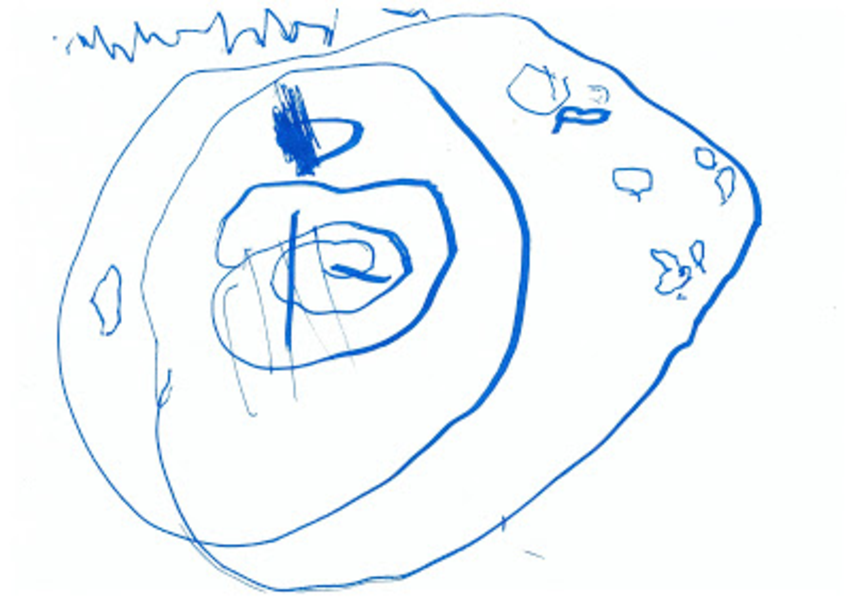
\includegraphics{bookdown-demo_files/figure-latex/Mapi-1.pdf}

3 urte eta 5 hile: ``pelikula bat mounstroana''

\textbf{OCIEA UEX OAEA}

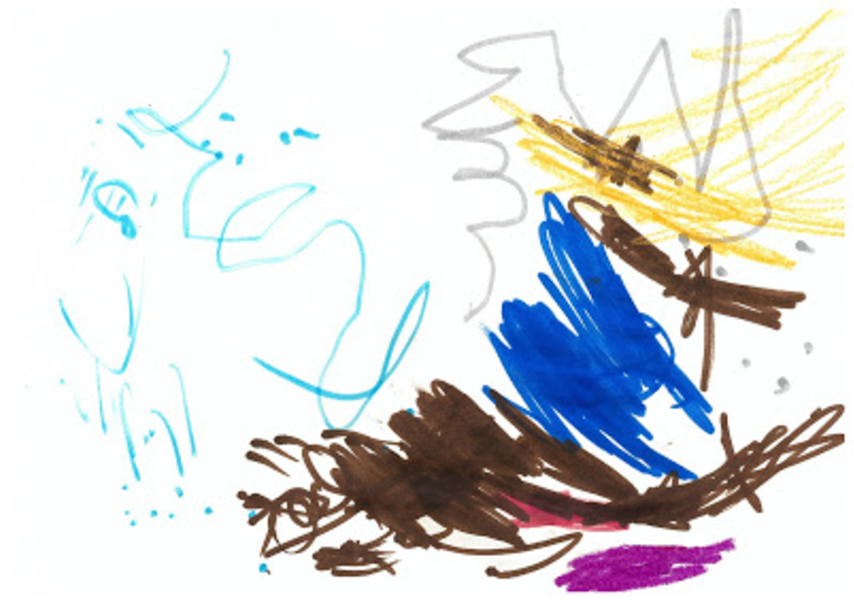
\includegraphics{bookdown-demo_files/figure-latex/Auza-1.pdf}

4 urte eta hilabete ``lo egitea eta muinekakaz jolastea''

\textbf{LORAK BIE}

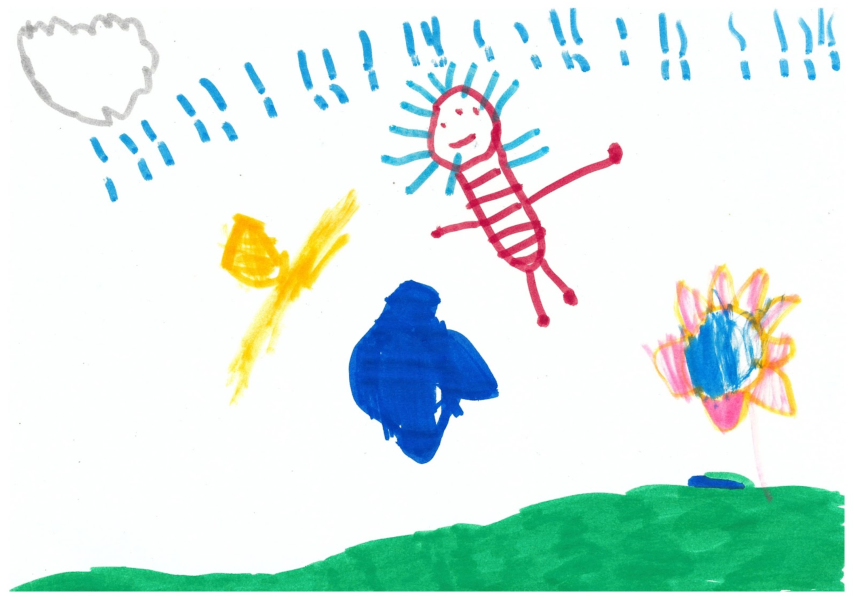
\includegraphics{bookdown-demo_files/figure-latex/Enara-1.pdf}

4 urte eta 5 hile: ``lorak batzie''

\textbf{DANSA EGTA}

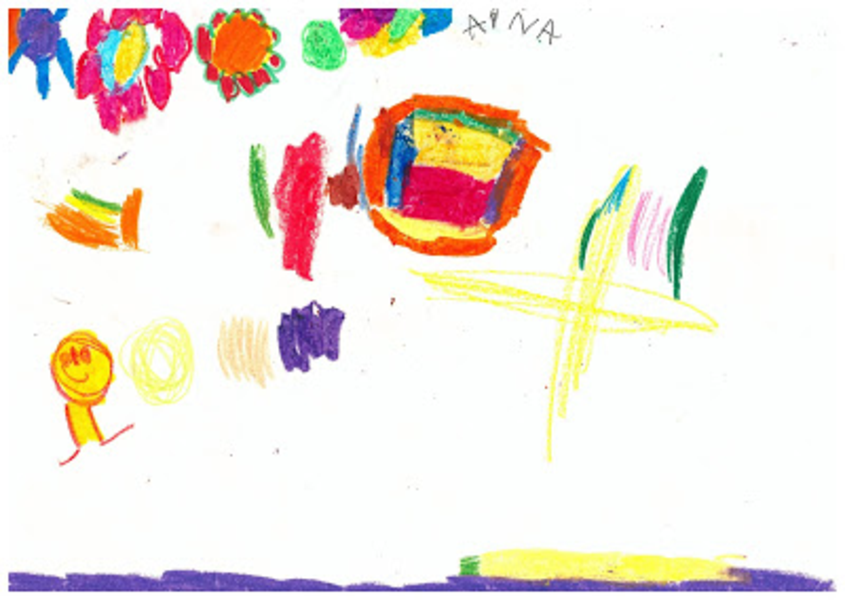
\includegraphics{bookdown-demo_files/figure-latex/Aina-1.pdf}

4 urte eta 7 hile: ``dantza egitea''

\textbf{KOPAKO COKOA}

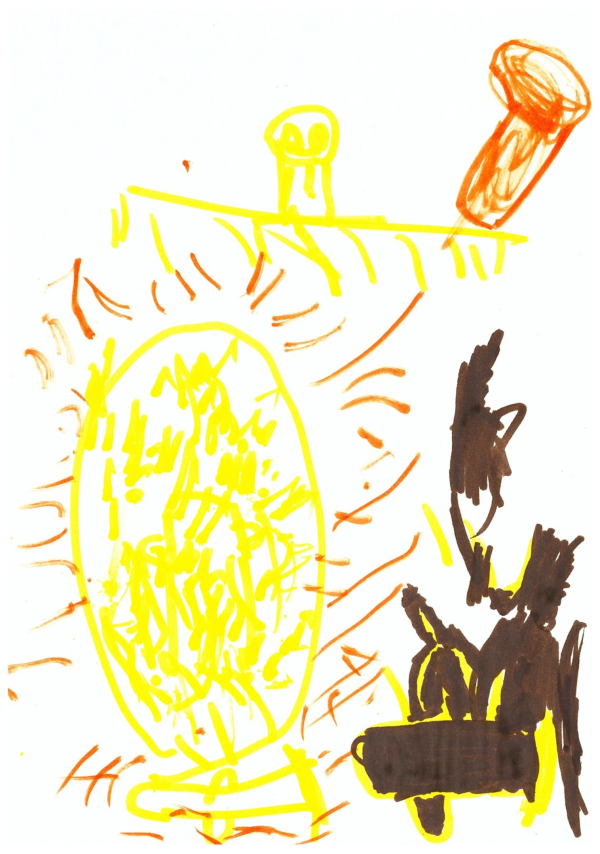
\includegraphics{bookdown-demo_files/figure-latex/Xabier-1.pdf}

4 urte eta 9 hile: ``kopako jokoa''

\textbf{MUEAI JOLSTA}

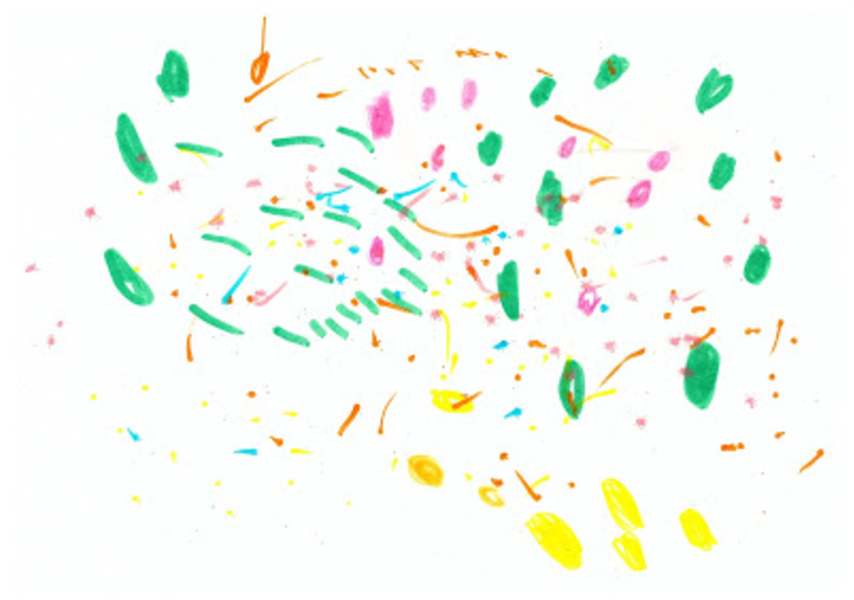
\includegraphics{bookdown-demo_files/figure-latex/Olaia-1.pdf}

4 urte eta 9 hile: ``muinekakin jolastea''

\textbf{PAIOJ OLASTEA}

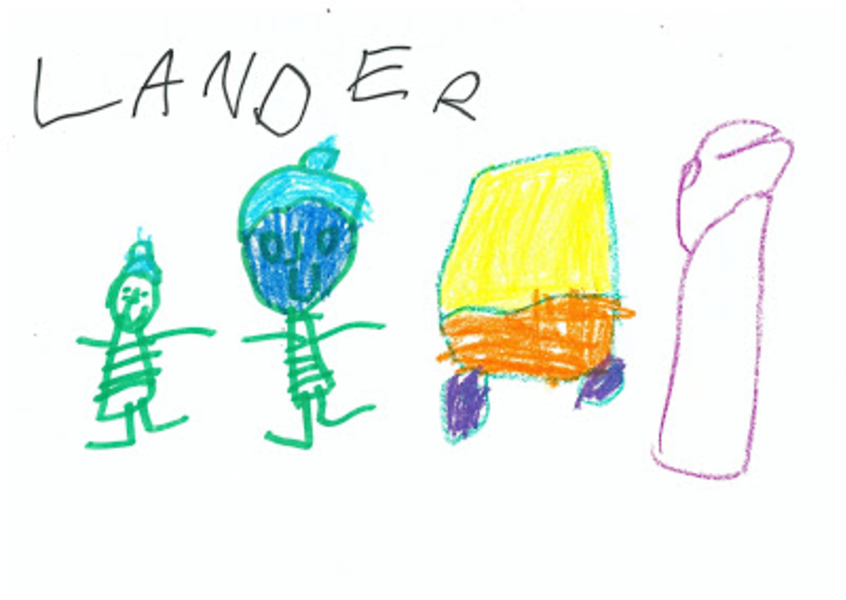
\includegraphics{bookdown-demo_files/figure-latex/Lander-1.pdf}

5 urte eta 4 hile: ``Playmobilakin jolastea''

\textbf{ESKUPPILOTAN GOLSTEA}

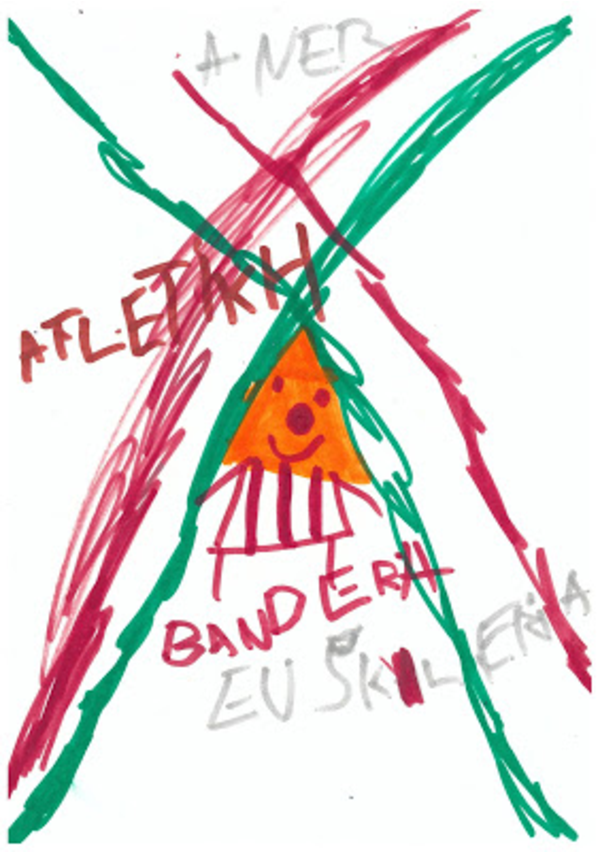
\includegraphics{bookdown-demo_files/figure-latex/Aner-1.pdf}

6 urte eta hile bi: ``eskupilotan jolastea''

--

\hypertarget{eskolan-gaur}{%
\section{Eskolan gaur}\label{eskolan-gaur}}

\hypertarget{irakurketaren-irakaskuntza-lehen-hezkuntzako-lehen-zikloan-6-eta-8-urteen-artean}{%
\subsection{Irakurketaren irakaskuntza Lehen Hezkuntzako lehen zikloan (6 eta 8 urteen artean)}\label{irakurketaren-irakaskuntza-lehen-hezkuntzako-lehen-zikloan-6-eta-8-urteen-artean}}

\begin{itemize}
\tightlist
\item
  Bestalde, idatzizko kodean, testu- eta formatu-motetan eta idatzizko hizkuntza erabiltzeko moduetan sakontzen dute.
\item
  Fonemaren eta grafemaren arteko harremana sendotzen dute.
\item
  Lehen Hezkuntzako lehen zikloa funtsezkoa da idatzizko kodeaz jabetzeko, eta gela arruntean (berezko esparruan) heldu behar diogu jabekuntza horri.
\end{itemize}

\hypertarget{irakurketaren-irakaskuntza-lehen-hezkuntzako-bigarren-eta-hirugarren-zikloetan-8-eta-11-urte-bitartean}{%
\subsection{Irakurketaren irakaskuntza Lehen Hezkuntzako bigarren eta hirugarren zikloetan (8 eta 11 urte bitartean)}\label{irakurketaren-irakaskuntza-lehen-hezkuntzako-bigarren-eta-hirugarren-zikloetan-8-eta-11-urte-bitartean}}

\begin{itemize}
\tightlist
\item
  \emph{Irakurtzen ikasteari} uzten diote eta \emph{ikasteko irakurtzen} hasten dira
\item
  Irakurketaren beste funtzio batzuk alde batera utzi gabe\\
  Besteak beste, aisia, plazera, pertsonen arteko komunikazioa eta komunikazio soziala.
\end{itemize}

\hypertarget{helburua-irakurtzen-duguna-ulertzen-irakastea}{%
\subsection{Helburua\ldots{} irakurtzen duguna ulertzen irakastea:}\label{helburua-irakurtzen-duguna-ulertzen-irakastea}}

\begin{itemize}
\tightlist
\item
  ``irakurketaren funtsa'' da irakurtzen duguna ulertzea, Durkin (1992:32)
\item
  Prozesu horren bidez eratzen baitugu testuaren esanahia.
\item
  Prozesu konplexua da testuen esanahia eratzea.
\item
  Ez da prozesu automatikoa, eta, motibazioak eta intentzioak ez ezik, pentsatzeko eta arazoak konpontzeko prozesuek hartzen dute parte, baita irakurleek dakitenak ere.
\end{itemize}

\hypertarget{irakurritakoaren-ulermen-estrategiak}{%
\section{Irakurritakoaren ulermen estrategiak}\label{irakurritakoaren-ulermen-estrategiak}}

Dekodetzea ez da arazoa eta hitzak identifikatzeko mekanismoak garatuta daude.
Testuari buruz aldez aurretik dakiena erabili behar du.
Ulermen estrategiak erabiltzea komenigarria da: Metakognizioaren garrantzia (zer eta nola egiten duen ohartzea).

Ruizek \& Aldekoak (2000) irakurtzeko estrategiak honela definitzen dituzte:

\begin{quote}
Arazoak konpontzeko edo helburu jakin bat lortzeko eman behar diren pausoak.
\end{quote}

Hiru multzotan sailkatzen dituzte esrategiok:

\begin{enumerate}
\def\labelenumi{\arabic{enumi}.}
\tightlist
\item
  Irakurketa aurrekoak\\
  garrantzitsuenak jatorrizko hiztun ez diren irakurleentzat.
\item
  Irakurri bitartekoak
\item
  Irakurri ondorengoak
\end{enumerate}

Estrategion helburua da zer ulertzen duten eta zer ez ohartaraztea, Sole (1992)

\hypertarget{eskema-eta-adibideak}{%
\section{Eskema eta adibideak}\label{eskema-eta-adibideak}}

Solék 1992an irakatsi beharko liratekeen estrategien honako eskema zehaztu zuen:

\begin{enumerate}
\def\labelenumi{\arabic{enumi}.}
\tightlist
\item
  Irakurketa \textbf{aurrekoak}:\\
  Helburuak zehazteko eta aldez aurretiko jakintza ateratzeko.\\
  Xedea ulertzea:

  \begin{itemize}
  \tightlist
  \item
    Zergatik irakurri behar dut? Zertarako irakurri behar dut?
    Kasuan kasuko edukiaren jakintza aktibatzeko:\\
  \item
    Zer dakit testu horren edukiaz? Testu motta horretaz? Zer dakit autore horretaz? Zer dakit testuinguruaz?
  \end{itemize}
\item
  Irakurri \textbf{bitartean}:\\
  Ulertzen dena berrikusteko eta egiaztatzeko, akatsen aurrean neurriak hartzeko bidea ematen duten jarduerak:\\
  Inferentziak:\\
  Zein izan liteke eleberri edo ipuin honen amaiera? Zer proposatuko nuke hemen planteatzen den arazoa konpontzeko? Zer esanahi izan lezake hitz ezezagun horrek?
  Berrikustea eta laburtzea:\\
  Zer azaldu nahi zen paragrafo, atal edo kapitulu honetan? Zer erlazio du aurrekoekin? Berregin al dezaket azaldutako argudioen haria?
  Zentzua neurtzea:\\
  Ba al du zentzurik testu honek? Koherentea al da? Ulertzen al da? Zer zailtasun ditu?
\item
  Irakurri \textbf{ondoren}:\\
  Irakurri bitartean lortutako ezagutza laburtzeko, sintetizatzeko eta hedatzeko jarduerak.\\
  Arreta ideia nagusira zuzentzea:\\
  Zein da testuak ematen duen informazio ezinbestekoa, irakurketa-helburua lortzekoa? Zer informazio jo ditzaket garrantzi gutxikoa? Eta funtsezkoa? Zer ekarpen egiten du testuak nik ez nekienik? Nola antolatuko ditut ideia nagusiak zentzua izango duen testu batean?
\end{enumerate}

\hypertarget{testu-motak-ere-garrantzia-du}{%
\section{Testu motak ere garrantzia du\ldots{}}\label{testu-motak-ere-garrantzia-du}}

Enseñar lenguan (Lomas \& Osoro, 1994) lau trebetasun bereiztu zituzten: hitz egitea, entzutea, irakurtzea eta idaztea. Trebetasun horien bitartez helburu komunikatiboa lortzen genuela adierazi zuen. Trebetasun horiei makrotrebetasunak deitu zien.

Makrotrebetasun horien azpian mikrotrebetasunak identifikatu zituen, trebetasun bakoitzean egin beharreko ekintzak dira, esaterako:

\begin{enumerate}
\def\labelenumi{\arabic{enumi}.}
\tightlist
\item
  Idazteko sistema: grafiak identifikatu, hitzak nola ordenatzen diren ikasi\ldots{}
\item
  Hitzak eta esaldiak: hitzak identifikatu eta esanahia\ldots{}
\item
  Gramatika eta sintaxia: perpausaren zatiak identifikatu\ldots{}
\item
  Testua eta komunikazioa (mezua): informazioa bilatu, testua zehatz ulertu, abiadura egokian irakurtzen jakin\ldots{}
\end{enumerate}

Horretarako proposamen didaktikoak aurkeztu zituen.

Gaur egun, berriz,\ldots{}

\href{https://www.youtube.com/embed/lsHc3SWiWEQ?rel=0}{
\includegraphics{bookdown-demo_files/figure-latex/unnamed-chunk-3-1.pdf}}

Prácticas letradas contemporáneas por Daniel Cassany: la perspectiva sociocultural (10 min).

\hypertarget{idaztea-eta-irakurtzea-lotura-duten-prozesu-bi-dira}{%
\section{Idaztea eta irakurtzea lotura duten prozesu bi dira?}\label{idaztea-eta-irakurtzea-lotura-duten-prozesu-bi-dira}}

\textbf{Tradizioan}: lehenengo irakurtzen eta gero idazten.

\textbf{Ondoren}: batera irakatsi eta ikasi beharreko jarduera bakartzat hartu zen, fase bi dituena: ``lectoescritura''.

\emph{Zergatik}? Biek testu idatzia hartzen dutelako oinarritzat.
Fons Esteve (2004: 20)

\hypertarget{garatuta-al-dituzte-ikasleek-gaitasunak-agintzen-zaizkien-testuak-sortzeko}{%
\subsection{Garatuta al dituzte ikasleek gaitasunak agintzen zaizkien testuak sortzeko?}\label{garatuta-al-dituzte-ikasleek-gaitasunak-agintzen-zaizkien-testuak-sortzeko}}

\begin{quote}
Se escribe mucho pero se enseña poco a escribir\ldots{} las prácticas explícitas de escritura, cuyo objetivo es incrementar las capacidades compositivas del alumnado, son escasas, breves y disciplinarias de lengua.\\
\emph{Cassany, Luna, \& Sanz (2000:128)}
\end{quote}

Egoera horri aurre egiteko zenbait proposamen sortu ziren ideia honetan oinarrituta:

Jakintza eraiki behar da ikasleak lehendik dakiena aprobetxatuz eta egoera komunikatibo jakinetan. Hori konstruktibismoaren ideia duzu, igarriko zenuenez.

Baina, ikuspegi konstruktibista ezin da uztartu metodologia didaktiko zehatz batekin, ez baitago \emph{metodologia didaktiko konstruktibista}rik; dagoena zera da: izaera konstruktibista duen estrategia didaktiko orokorra.

\hypertarget{hizkuntza-idatzia-eta-konstruktibismoa}{%
\section{Hizkuntza idatzia eta konstruktibismoa}\label{hizkuntza-idatzia-eta-konstruktibismoa}}

Zer ikasten dugu irakurtzen ikasten dugunean? Zer ikasten dugu idazten ikasten dugunean?

Konstruktibisten arabera, mezuak interpretatzen eta ekoizten ikasten dugu.

Irakurtzea eta idaztea ekintza sinbolikoak dira. \emph{Zergatik}? Ez direlako diruditena (gainazal baten gaineko trazu batzuk), baizik eta adierazten dutena.

Zergatik esaten da umeak hizkuntza idatzia eraiki egiten duela?

Umea aktiboa da, ingurunetik datorkion informazioa etengabe
interpretatzen eta berrantolatzen ari delako. Umeek hasiera batean ez dute ikusten idazkera hizkuntzari lotua. Hori prozesu geldo eta luze baten helmuga da.
Idazkera sistema interpretatu nahian, hipotesiak formulatu, frogatu eta birformulatu egin beharko ditu.

\hypertarget{kapituluko-erreferentziak}{%
\section{Kapituluko erreferentziak}\label{kapituluko-erreferentziak}}

Cassany, D., Luna, M., \& Sanz, G. (2000). \emph{Enseñar lengua} (6. arg.). Bartzelona: Graó.

Durkin, D. (1992). \emph{Teaching Them to Read} (6. argitalpena). Boston: Pearson.

Euskaltzaindia. (1998). Euskara batuaren ahoskera zaindua (EBAZ). \emph{Euskera: Euskaltzaindiaren lan eta agiriak}, 43, 485--490.

Eusko Jaurlaritzaren Legebiltzarra. (2015). 236/2015 Dekretua, abenduaren 22koa, Oinarrizko Hezkuntzaren curriculuma zehaztu eta Euskal Autonomia Erkidegoan ezartzen duena. \emph{Euskal Herriko Agintaritzaren Aldizkaria, 2016ko urtarrilaren 15a}, \emph{141}. Berreskuratua \url{https://www.euskadi.eus/y22-bopv/eu/bopv2/datos/2016/01/1600141e.shtml} -(e)tik

Fons Esteve, M. (2004). \emph{Leer y escribir para vivir: alfabetizacion inicial y uso real de la lengua escrita en el aula}. Bartzelona: Graó.

Lomas, C., \& Osoro, A. (1994). Enseñar Lengua. In \emph{El enfoque comunicativo de la enseñanza de la lengua} (or. 17--30). Bartzelona: Paidós Ibérica.

Ministerio de Educación y Ciencia. (2007). \emph{PIRLS 2006. Estudio internacional de progreso en comprensión lectora de la IEA. Informe español}. Madril: Ministerio de Educación y Ciencia.

Mullis, I. V. ., \& Martin, M. O. (Arg.). (2016). \emph{PIRLS 2016. Marco de la evaluación} (2. arg.). Madril: Ministerio de Educación Cultura y Deporte. Berreskuratua \url{https://www.mecd.gob.es/inee/dam/jcr:d79b8f8b-d4a8-42b7-b63e-42aed382a8e7/pirls2016webokk.pdf} -tik

OECD. (2014). El programa PISA de la OCDE. Qué es y para qué sirve. OECD. Berreskuratua \url{https://www.oecd.org/pisa/39730818.pdf} -tik

Oñederra, M. L., Elordui, A., Epelde, I., Etxeberria, P., Jauregi, O., \& Salaberria, J. (2015). Euskaltzaindiaren Ahoskera batzordearen txostena (Ahoskerak axola du). \emph{Euskera: Euskaltzaindiaren lan eta agiriak}, 60(2), 499--531.

Ruiz, U., \& Aldekoa, I. (2000). La comprensión lectora. In U. Ruiz (Arg.), \emph{Didáctica de la segunda lengua en educación infantil y primaria} (or. 217--248). Madril: Síntesis.

Solé, I. (1987). Las posibilidades de un modelo teórico para la enseñanza de la comprensión lectora. \emph{Infancia y Aprendizaje}, \emph{10}(39--40), 1--13. \url{https://doi.org/10.1080/02103702.1987.10822170}

Solé, I. (1992). \emph{Estrategías de lectura}. Bartzelona: Graó.

\hypertarget{zenbait-baliabide-eta-kontsultarako-material}{%
\chapter*{Zenbait baliabide eta kontsultarako material}\label{zenbait-baliabide-eta-kontsultarako-material}}
\addcontentsline{toc}{chapter}{Zenbait baliabide eta kontsultarako material}

Oinarrizko gaztelaniazko baliabide bat: \url{http://leer.es/}

Madrilen Daniel Cassanyk leer.es-eko markoan emandako hitzaldia: Prácticas letradas contemporáneas, lehenengo zatia, \href{https://www.youtube.com/embed/lsHc3SWiWEQ}{la perspectiva sociocultural}, klasean ikusia behar genuke. Hitzaldia osorik eta beste elementu batzuk ere bai: \href{http://www.youtube.com/watch?v=lsHc3SWiWEQ\&list=PLB91A13AEFDB0D9B0\&index=3}{hemen}.

\hypertarget{sarrera-egiteko}{%
\section{Sarrera egiteko}\label{sarrera-egiteko}}

Zuen hautu tekniko eta metodologikoak oinarritzeko, \href{https://github.com/JuanAbasolo/HD/raw/03-gaia/05_hizkuntzen_irakaskuntzarako_metodoak.pdf}{hemendik} jaits dezakezuen dokumentua erabiltzea komeni da (gorde dokumentua).

\hypertarget{baliabideak-sortzeko}{%
\section{Baliabideak sortzeko\ldots{}}\label{baliabideak-sortzeko}}

Eduteka, \href{http://eduteka.icesi.edu.co/articulos/NarracionesDigitales_Educause}{Siete elementos esenciales de las Narraciones Digitales}, ICESI (Cali, Kolombia)

\begin{quote}
Traducción al español del documento de Educause que se enfoca en los
siete elementos que todo educador debe conocer sobre narraciones
digitales: 1) ¿qué son? 2) ¿quiénes están trabajando en ellas? 3) ¿cómo
funcionan? 4) ¿por qué son significativas? 5) ¿qué aspectos negativos
tienen? 6) ¿para dónde van? y 7) ¿cuáles son sus implicaciones para la
enseñanza y el aprendizaje?.
\end{quote}

Cuaderno Intercultural, \href{http://www.cuadernointercultural.com/materiales/lectura/cuentos-fabulas-y-leyendas/\#cuentosdidact}{Cuentos infantiles y explotaciones didácticas}.
Baliabide honetan hainbat baliabide aurkituko dituzue. Nabarmentzen ari garen ipuinen erabilera didaktikoaz gain, beste hainbat aukera ere erakutsi eta estekatzen dituzte; Espainiako ikuskeratik egindakoa izan arren, beste toki batzuetako zenbait baliabide ere harrtzen ditu kontuan, beti ere gaztelaniaz.

Mario Aller (2011-11-13) \href{http://www.educacontic.es/blog/la-narrativa-digital-y-la-escuela}{La narrativa digital y la escuela} \emph{EducaconTIC}, INTEF

\begin{quote}
Dicen que contar historias es una actividad parecida al arte. Y la
literatura es considerada como una de las artes más perfectas porque utiliza las palabras,
que son el medio más reconocido para expresar la belleza. La narrativa
trata, precisamente, de la manera de contar historias de una manera
efectiva, interesante y, sobre todo, emocionante y hermosa. Sin embargo,
hoy en día las historias no sólo se cuentan con palabras, sino
especialmente con imágenes; y no solo eso, sino con imágenes y sonidos.
Así, se ha originado una nueva categoría en las tecnologías de la
información y la comunicación, \href{http://www.storycenter.org/}{una nueva narrativa}.
\end{quote}

\hypertarget{estrategiak}{%
\section{Estrategiak}\label{estrategiak}}

¿Qué significa enseñar estrategias de lectura? izan zen 2010 Escorialeko udako ikastaroetan Isabel Solék emaniko hitzaldia. Horretariko lau bideo labur oso gomendagarri dira, sekuentzia didaktikorako zenbait erabaki era oinarrituan egiteko:

\begin{itemize}
\tightlist
\item
  \href{http://leer.es/web/leer/-/estrategias-de-lectura-1-introduccion}{Irakurketarako estrategiak}
\item
  \href{http://leer.es/web/leer/-/estrategias-de-lectura-10-ayudas-previas}{Aurretiko laguntzak}
\item
  \href{http://leer.es/web/leer/-/estrategias-de-lectura-12-despues-de-leer}{Irakurri ondorengoak}
\item
  \href{http://leer.es/web/leer/-/estrategias-de-lectura-11-durante-la-lectura}{Irakurri bitartean}
\end{itemize}

Daniel Cassanyk sortutako baliabideak, ezagutu beharrekoak (eta goiko bideoetan erreferentziatzat hartzen dituenak):

\begin{itemize}
\tightlist
\item
  \href{http://educalab.es/documents/235507/242734/ep_eso_prof_10clavesparaensenarainterpretar.pdf}{Irakurtzen \textbf{irakasteko} irizpideak}
\item
  \href{http://leer.es/documents/235507/353837/art_alum_ep_eso_leereradigital_10clavesparaaprenderrainterpretar_danielcassany.pdf}{Irakurtzen \textbf{ikasteko} irizpideak}
\end{itemize}

\hypertarget{gehiago-jakiteko-baliabide-bibliografiko-batzuk}{%
\subsection{Gehiago jakiteko baliabide bibliografiko batzuk}\label{gehiago-jakiteko-baliabide-bibliografiko-batzuk}}

Díaz Blanca, L. (2002). \href{http://www.scielo.org.ve/scielo.php?script=sci_arttext\&pid=S0798-97922002000200007\&lng=es\&nrm=iso}{La Escritura: Modelos Explicativos e Implicaciones Didácticas}. \emph{Revista de Pedagogía}, \emph{23}(67), 319--332.

Ibarra, I. (2009, irailak 5). Konstruktibismoa, hizkuntza idatzia eta eskola. UPV/EHU. Berreskuratua \url{https://ikasmaterialak.ehu.eus/hezkuntza/konstruktibismoa/Konstruktibismoa.pdf} -(e)tik

\begin{quote}
Hizkuntza idatziari eta eskolari buruz konstruktibistek idatzitako zenbait testu bilduta dituzue jarraian: Emilia Ferreiro‐ren eta Ana Teberosky‐ren hasierako ikerketetatik gaur egunera arte konstruktibismoaren eta hizkuntza idatziaren inguruan dihardutenen ahotsak dira. Ahots horien bidez konstruktibistek idazkerari eta horren inguruko auziei buruz zer dioten ulertuz joango gara. Niri argigarri suertatu zaizkit, eta zuentzat ere hala izatea espero dut. Liburu honek bi zati ditu: 10 orri inguruko sarrera bat (bibliografia atzean dago), eta, ondoren, pasarte edo aipuak, euskarara itzuliak. 1979tik gaur egunera bildutako pasarteak dira eta urteez gain liburuen barruan dauden zatiak direla gogoratu behar dugu, hots, testuinguru bat daukatela. Bibliografian dituzue aipatuta «jatorrizko testu» guztiak, liburuaren osotasunean hobeto uler ditzazuen eta gehiago jakin dezazuen. Testua arintzeko, irudiak, argazkiak\ldots{} jarri ditut.\\
Hizkuntza idatzia lantzerakoan jarraitzen diozuen ildoari jarraitzen diozuela, ondoko lerroetan datorrena irakurtzera gonbidatzen zaituztet\ldots{} eta ondoren, ERAIKI!
\end{quote}

Ulzurrun, A. D. de, Pinyol, N. F., Ràfols, R. F., Cardete, M. R. M., Rovira, D. R., Pujol, V. S., \ldots{} Olivella, F. C. (2000). \emph{El aprendizaje de la lectoescritura desde una perspectiva constructivista.} (M. D. M. B. COLET, Itzul.) (1. arg.). Bartzelona: Graó.

UPV/EHUko liburutegian zenbait ale.

\hypertarget{oharra}{%
\section{Oharra}\label{oharra}}

Zuen lana egiteko prozesuan aurkitzen dituzuen baliabide onak eta interesgarriak partekatu ikasgaiko txatean komentario/balorazio labur batez.

\hypertarget{hirugarren-jarduera-23}{%
\chapter*{Hirugarren jarduera (2/3)}\label{hirugarren-jarduera-23}}
\addcontentsline{toc}{chapter}{Hirugarren jarduera (2/3)}

Oraingoan zuok sortu behar duzue sekuentzia didaktikoa. Horren (auto/kanpo) ebaluazioa Heziberri 2020ko dokumentazioa erabiliko dugu, propio horretarako sortutakoa.

Sekuentzia didaktiko honetan agertzen diren baliabide guztiak zuok sortutakoak izan behar dute; hau da, jabetza intelektuala zuok izan behar duzue.

\hypertarget{hizkuntzen-irakaskuntzarako-metodoak}{%
\chapter{Hizkuntzen irakaskuntzarako metodoak}\label{hizkuntzen-irakaskuntzarako-metodoak}}

\href{../Diapoak/05_Metodoak.html}{
\includegraphics{assets/badge.png}}

Zenbait galdera hasieran erantzuteko:

\begin{enumerate}
\def\labelenumi{\arabic{enumi}.}
\tightlist
\item
  Badago alderik, zure ustez, \emph{ikuspegia}, \emph{metodoa} eta \emph{teknika} kontzeptuen artean?
\item
  Zerk osatzen du hizkuntzen irakaskuntzarako metodoa?
\item
  Zein metodo daude hizkuntzen ikaskuntza eta irakaskuntzarako?
\item
  Zein ezaugarri dituzte?
\end{enumerate}

Galderon lehenengo erantzun bat eman behar zenuke(te), argiago ulertzeko segidan datorren teoria-eta. Horretan aurreko galderei erantzun oinarritu bat ematen saiatu nahi da.

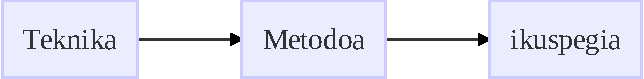
\includegraphics{bookdown-demo_files/figure-latex/unnamed-chunk-4-1.pdf}

`Edward Anthony, 1963',

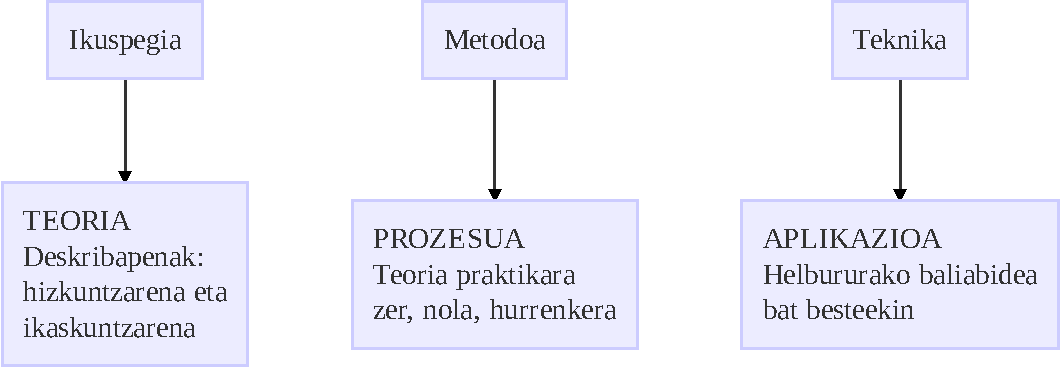
\includegraphics{bookdown-demo_files/figure-latex/unnamed-chunk-5-1.pdf}

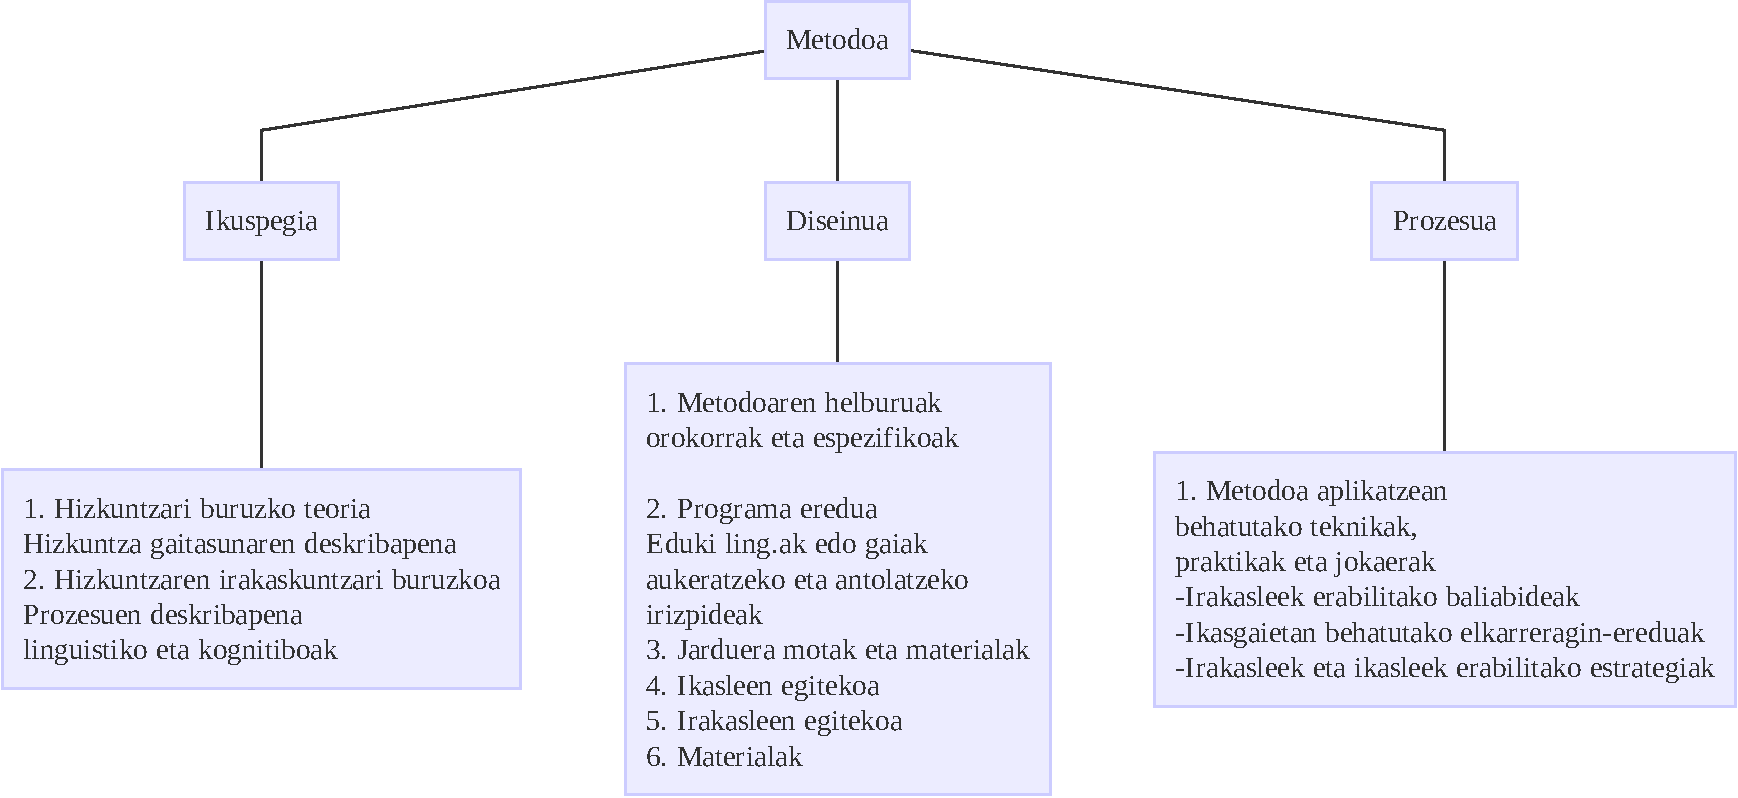
\includegraphics{bookdown-demo_files/figure-latex/unnamed-chunk-6-1.pdf}

(Richards, C eta Rodgers, S, 2009)

\hypertarget{hizkuntzari-buruzko-teoriak}{%
\section{Hizkuntzari buruzko teoriak}\label{hizkuntzari-buruzko-teoriak}}

Kontzeptu batzuk oinarrizkoak dira hizkuntzen ikas-irakaskuntzaz aritzeko:

\begin{description}
\tightlist
\item[Hizkuntza jabekuntza]
Gizakien berezko prozesua eta inkontzientea

Hizkuntzaren arauak berez barneratzen dira

Hizkuntzaren erabilera naturalean egina

Komunikatzeko helburua

Hizkuntza-formari arreta gutxi
\item[Hizkuntza ikaskuntza]
Prozesu kontzientea

Hizkuntzaren sistema ikasia

Ikasketa formala
\item[Bigarren Hizkuntza]
Hizkuntzak komunikazioan funtzio soziala eta instituzionala betetzen du

Komunitate batzuek hizkuntza sistema bi dituzte arrazoi historiko eta sozialek eratuak.

Adibidez: gaztelania (edo euskara) EHan ikastea
\item[Atzerriko Hizkuntza]
Testuinguru instituzionalean ikasten da eta ez du funtzio sozialik gizarte horretan.

Adibidez, gaztelania Portugalen (eskola edo unibertsitatean) ikastea
\end{description}

\hypertarget{iraganean}{%
\subsection{Iraganean}\label{iraganean}}

\textbf{XVIII. eta XIX. mendeetan} hizkuntza modernoen irakaskuntza bideratzen zen gramatika arauemailearen ikaskuntzara; horretarako \emph{gramatika-itzulpenezko metodoa}k ikaslea eramaten zuen gramatika era induktiboan ikastera, hitzen zerrenda elebidunak buruz ikastera eta itzulpenak egitera.

\textbf{XIX. mendearen amaieran} hizkuntza eta literaturaren ikaskuntzari begiratu zitzaion. Horretarako, hizkuntza arauak era induktiboan ikasi behar zituen ikasleak eta literaturaren irakasuntzari begiratzen hasi zitzaion. \emph{Metodo zuznea} deritzo ordukoari. Ezaugarri nabarmenak dira ahozko elkarreraginaren erabilera, xede hizkuntzaren bidez edukiak ikastea eta gramatikari buruzko ikaskuntzak era deduktiboan lantzen ditu.

\hypertarget{ko-hamarkadan}{%
\subsection{50ko hamarkadan}\label{ko-hamarkadan}}

\begin{description}
\tightlist
\item[Metodo audiolinguala]
EEBBetan. Mintzaira hartzen zen hizkuntzaren oinarritzat
\item[Metodo situazionala]
Erresuma batuan, edukiak egoera jakinetan aurkezten eta lantzen ziren.
\item[Metodo estruktural-globala]
Izena, berez, \emph{ikus-entzunezko metodo estruktural-globala (IEEG, SGAV)} du; Frantzian garatu zen eta hizkuntza laborategiak ziren euren ezaugarri behinena.
\end{description}

\hypertarget{ko-hamarkadaren-erditik-aurrera}{%
\subsection{80ko hamarkadaren erditik aurrera}\label{ko-hamarkadaren-erditik-aurrera}}

\textbf{Planteamendu komunikatiboa} garatu zen orduan; horretan, egiazko komunikazio egoerak indartzen dira. Komunikazioaren unitatetzat testua hartzen da; erabiltzen diren testuak egiazkoak dira eta testuinguratuta lantzen dira, testuinguru jakinetan. Komunikazioa bultzatzeko, lanketak elkarlanean egiten dira (bikoteka, taldeka \ldots). Helburua izaten du hizkuntzaren lau trebetasunen lanketa.

\hypertarget{xxi.-mendean}{%
\subsection{XXI. mendean}\label{xxi.-mendean}}

Europako Erreferentzia Marku Bateratua (Europako Kontseilua, 2002) bihurtu da hizkuntzaren ikaskuntzaz pentsatzeko ardatz. Errealitate eleaniztunari begiratzen dio. Horretarako hizkuntzan murgiltzea du helburu, Edukien Bitarteko Hizkuntzen Ikaskuntza\footnote{Ingelesezko \emph{CLIL} akronimoaz aipatzen da askotan}; planteamenduak ekintzetan oinarritzen dira eta atazen bitarteko ikaskuntza bideratu nahi izaten da. Elkarrizketa berarizko trebetasuntzat orduan hasten da hartzen.

Oinarrizko Gaitasunen formulazioan sustraituta dago metodoa eta curriculumaren planteamenduetan txertatzen dira. Gizarte berriaren ikasteko eredu berriei erantzuteko mugimendua antzematen da.

Gaitasun komunikatiboa (edo \emph{komunikazio-gaitasuna}) oinarrizko gaitasunetarikotzat hartzen da.

Ikastetxeetako antolakuntzan aldaketak eragin dira Ikastetxearen Hizkuntza Proiektua (IHP) eta eleaniztasunerako planteamenduak ahalbidetzeko.

\textbf{Planteamendu komunikatiboaren ezaugarriak}

\begin{enumerate}
\def\labelenumi{\arabic{enumi}.}
\tightlist
\item
  Eskolako irakaskuntzak badu zerikusirik hizkuntzaren erabilerarekin eta ez hizkuntzaren jakintzarekin
\item
  Hizkuntzak eguneroko bizimoduaren komunikazio-egoera errealetan erabiltzeko ikasten dira
\item
  Ikasleak/hiztunak oinarrizko trebetasunak garatu behar ditu: ulermenezkoak (irakurri, entzun) eta adierazkorrak (hitz egin, idatzi)
\item
  Egoera errealetan hizkuntza erabiltzeak ikasketa eraginkorragoa egiten du
\item
  Ikaslea da ikaste-prozesuaren ardatza
\item
  Irakaslea ez da ikasketaren erdigunea, eta toki hori ikasleari utzi behar dio ikasketa autonomoagoa egin dezan
\item
  Ikaslearen beharrizanak, asmoak eta ikasteko modu anitzak kontuan hartu behar dira, bai eta ikaslearen esperientziak beste hizkuntzen ikasketetan
\item
  Material irekiak erabili behar dira: helburuen arabera behar dena gehituz, kenduz edo egokituz
\item
  Oreka bat bilatu behar da zuzentasun gramatikalaren eta komunikazio eraginkorraren artean
\item
  Dena den, gramatika komunikazioaren zerbitzuan dago (eta ez alderantziz)
\end{enumerate}

\hypertarget{estrukturalismoa-50}{%
\subsection{Estrukturalismoa ('50)}\label{estrukturalismoa-50}}

Behaviorismoa eta linguistika estrukturalean oinarritzen da. Hizkuntza arau jakinak dituen ohitura sistema da. Beraz, irakaskuntzan:

\begin{itemize}
\tightlist
\item
  Garrantzia du jatorrizko hiztunek elakrrizketan erabiltzen dituzten \textbf{esaldiak imitatu eta buruz ikasteak}.
\item
  Hizkuntza ikastea \textbf{ohitura linguistikoak} ikastea da. Behin eta berriro \textbf{errepikatu} behar dira egiturok.
\item
  Ahalegin handia egiten da ikasleak \textbf{ez dezan okerrik egin}.
\item
  \textbf{Egiturak progresiboki ordenatzen} dira eta banan banan irakasten.
\item
  Garrantzi berezia ematen zaio ahoskerari.
\item
  \textbf{Gramatika deduktiboki azaltzen da} adibideen bitartez.
\item
  \textbf{Entzun-ikusgailuak} erabiltzen dira: zintak, hizkuntza laborategiak eta metodo bisualak
\end{itemize}

\hypertarget{nozional-funtzionala-70}{%
\subsection{Nozional-funtzionala ('70)}\label{nozional-funtzionala-70}}

Hizkuntzaren dimentsio semantiko-komunikatiboari begiratzen zaio. Hizkuntza tresnatzat hartzen da, funtzio joakin bat lortzeko erabiltzen dena. Beraz, irakasuntzan:

\begin{itemize}
\tightlist
\item
  Edukiak antolatnze dira adieraren eta tuntzioaren arabera (National Syllabuses, Wilkins, 1976)
\item
  Gramatikaren irakaskuntzari ez zaio garrantzi handirik ematen.
\item
  Hizketarako egiturak irakatsi behar dira.
\item
  Nozioen (hitzen esangura, denbora\ldots) eta funtzioen (agurtzea, aurkeztea\ldots) arteko loturari garrantzia.
\item
  Irakaskuntza programek honakoak zehaztu behar ditu ikaslea komunikatzeko:
\item
  Gramatika
\item
  Lexikoa
\item
  Gaiak
\item
  Nozioak
\item
  Kontzeptuak
\end{itemize}

\hypertarget{interaktiboa-80}{%
\subsection{Interaktiboa ('80)}\label{interaktiboa-80}}

Hizkuntza ulertzen da elkarreragin moduan, norberaren garapenerako eta elkarreragin sozioalerako. Beraz, honela ulertu behar da irakasuntza:

\begin{itemize}
\tightlist
\item
  Elkarreraginean agertzen diren egiturak aztertu eta irakatsi:
\item
  Negoziazioa
\item
  Ekintza
\end{itemize}

\begin{quote}
Los estudiantes logran la facilidad en el usa de una lengua cuando su atención se centra en transmitir y recibir mensajes auténticos.
\emph{Rivers1987}
\end{quote}

\textbf{Adibideak}: Hizkuntza jardueren bidez ikastea, programazio neurolinguistikoa, hizkuntzaren ikaskuntza kooperatiboa, Edukietan oinarritutako irakaskuntza.

\hypertarget{galdera-nagusi-bi-erantzuteko}{%
\subsection{Galdera nagusi bi erantzuteko:}\label{galdera-nagusi-bi-erantzuteko}}

\begin{quote}
Zer prozesu kognitibok eta psikolinguistikok hartzen du parte hizkuntzaren ikaskuntzan?
\end{quote}

\begin{quote}
Zein baldintza dira nahitaezkoak ikaskuntza-prozesu horiek aurrera eramateko?
\end{quote}

\begin{enumerate}
\def\labelenumi{\arabic{enumi}.}
\tightlist
\item
  KRASHEN-en Monitorearen Eredua (1981) eredu naturala
  Jabekuntza eta ikaskuntza bereizten ditu.
\end{enumerate}

Stephen Krashen (1987) psikolinguistak hizkuntza‐informazioa prozesatzeko --eta ondorioz hizkuntza gaitasuna lortzeko ere‐ bi prozesu bereizi zituen: jabekuntza (acquisition) eta ikaskuntza (learning), hurrenez hurren.

\hypertarget{hizkuntzen-jabekuntza}{%
\subsubsection{Hizkuntzen jabekuntza}\label{hizkuntzen-jabekuntza}}

\begin{longtable}[]{@{}lll@{}}
\toprule
\begin{minipage}[b]{0.30\columnwidth}\raggedright
Ezaugarriak\strut
\end{minipage} & \begin{minipage}[b]{0.30\columnwidth}\raggedright
Prozesua\strut
\end{minipage} & \begin{minipage}[b]{0.30\columnwidth}\raggedright
Emaitza\strut
\end{minipage}\tabularnewline
\midrule
\endhead
\begin{minipage}[t]{0.30\columnwidth}\raggedright
PraktikoaErabilerari lotua (elkarreragina).Ez-kontzientea.Okerrez jabetzen garen arren, ez dakigu zergatia (gramatika arauak)\strut
\end{minipage} & \begin{minipage}[t]{0.30\columnwidth}\raggedright
Egoera komunikatiboan input ulergarria jaso ondoren berez sortzen den hizkuntza-gaitasuna\strut
\end{minipage} & \begin{minipage}[t]{0.30\columnwidth}\raggedright
Era automatikoan sortzen eta ateratzen diren hitzak eta esaldiak\strut
\end{minipage}\tabularnewline
\bottomrule
\end{longtable}

\hypertarget{hizkuntzen-ikaskuntza}{%
\subsubsection{Hizkuntzen ikaskuntza}\label{hizkuntzen-ikaskuntza}}

\begin{longtable}[]{@{}lcl@{}}
\toprule
\begin{minipage}[b]{0.81\columnwidth}\raggedright
Ezaugarriak\strut
\end{minipage} & \begin{minipage}[b]{0.05\columnwidth}\centering
\strut
\end{minipage} & \begin{minipage}[b]{0.05\columnwidth}\raggedright
\strut
\end{minipage}\tabularnewline
\midrule
\endhead
\begin{minipage}[t]{0.81\columnwidth}\raggedright
Indukzio eta dedukzio prozesu logikoen emaitza.Arau, definiziko, printzipio eta informazio-unitateen ezagutza esplizituaArreta kontzienteaArrazoiaren eremuaMetahizkuntza: hizkuntzari buruzko ezagutza teorikoa.Itzulpen-mekanismoa: H1ean esaldiak sortu eta hizkuntza ezagutza formala erabilz H2ko esaldi bihurtu.Monitorearen teoria.\strut
\end{minipage} & \begin{minipage}[t]{0.05\columnwidth}\centering
\strut
\end{minipage} & \begin{minipage}[t]{0.05\columnwidth}\raggedright
\strut
\end{minipage}\tabularnewline
\bottomrule
\end{longtable}

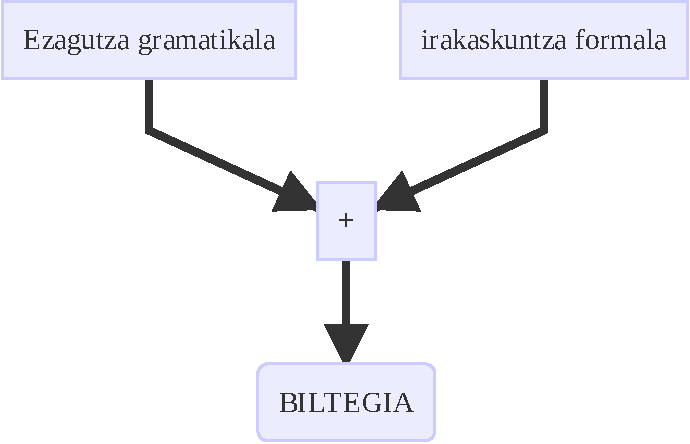
\includegraphics{bookdown-demo_files/figure-latex/unnamed-chunk-7-1.pdf}

\textbf{Eta praktikan zer?}

Praktikan maiz ikusten ditugu bata eta bestea hiztun baten jardueran. Ez dira nahastu behar:

\begin{itemize}
\tightlist
\item
  Berezko ezagutza eskuratzea \textbf{jabekuntza} prozesuaren ardura da.
\item
  Arrazoiaren bitarteko ezagutza \textbf{ikaskuntzari} dagokio.
\end{itemize}

\hypertarget{nola-jabetzen-da-bigarren-hizkuntzaz-pertsona-bat}{%
\subsubsection{Nola jabetzen da bigarren hizkuntzaz pertsona bat?}\label{nola-jabetzen-da-bigarren-hizkuntzaz-pertsona-bat}}

Krashenek (1987) dioenez hizkuntzaz jabetzen gara \textbf{I+1 ulertzean}.

Ekuazio horretako elementuak hauek dira:

\begin{description}
\tightlist
\item[I]
Hizkuntza inputa
\item[+1]
Ulertzen dena baino maila bat gehiago
\end{description}

Hizkuntza-inputaren bitartez hizkuntzaren jabe izateko beharrezkoa da:

\begin{itemize}
\tightlist
\item
  Inputa ulergarria izatea.
\item
  Arreta edo interesa piztu behar du.
\item
  Hizkuntza osotasunean agertu behar da, ez arau gramatikalak soilik.
\item
  Xede-hizkuntza hitz egiten den eremuan murgilduta.
\end{itemize}

\hypertarget{haurrak-nola-jabetzen-dira-hizkuntzaz}{%
\subsubsection{Haurrak nola jabetzen dira hizkuntzaz}\label{haurrak-nola-jabetzen-dira-hizkuntzaz}}

Itziar Laka (2005)

Jaio aurretik: Amaren hizkuntzaren doinu batzuk bereizten ditu.

Jaio bezain laster: Soinuak izan daitezkeen fonema guztiak bereizteko gaitasuna du. Gero hori galdu egiten da. Lehen 4-5 hilabeteetan.

\begin{description}
\tightlist
\item[Adibideak]
Japoniarrek eta txinatarrek \emph{R} eta \emph{L}. Denok berdin erabiltzen duzue gaztelaniazko \emph{J}? Entzun.

Euskara ikasten duten helduek ergatiboaren \emph{K}.
\end{description}

Hizkuntza jakinen fonologia bereganatu ahala, soinuak bereizteari uzten zaio.

6 hilabetetik aurrera: Egiturez jabetzen hasten dira. Helduen hitz jarioan silabak non diren sumatzen dute. Frekuentziak ateratzen dituzte. Fonologiaz eta silabez jabetzean ``ma'', ``pa''\ldots{} silabak egiten dituzte. Mundu osoko ume guztiak silaba berberak egiten dituzte hasieran: ezpainkaria (b, m, p)+bokala.

Ondoren\ldots{} espezialiazazioa: hizkuntzari dagozkion soinu bereziak egiten dituzte.

3 urterekin: Hizkuntza ikasi du: atal guztien jabekuntza ez da aldi berean egiten (ikertzen ari dira).

\hypertarget{metodoaren-diseinua}{%
\section{Metodoaren diseinua}\label{metodoaren-diseinua}}

Metodoa diseinatzeko orduan, ikasleen eta irakasleen jardunak antolatzeko irizpideak eta baliabideen erabilerarako irizpideak ezarri behar dira.

\hypertarget{ikaslearen-zeregina}{%
\subsection{Ikaslearen zeregina}\label{ikaslearen-zeregina}}

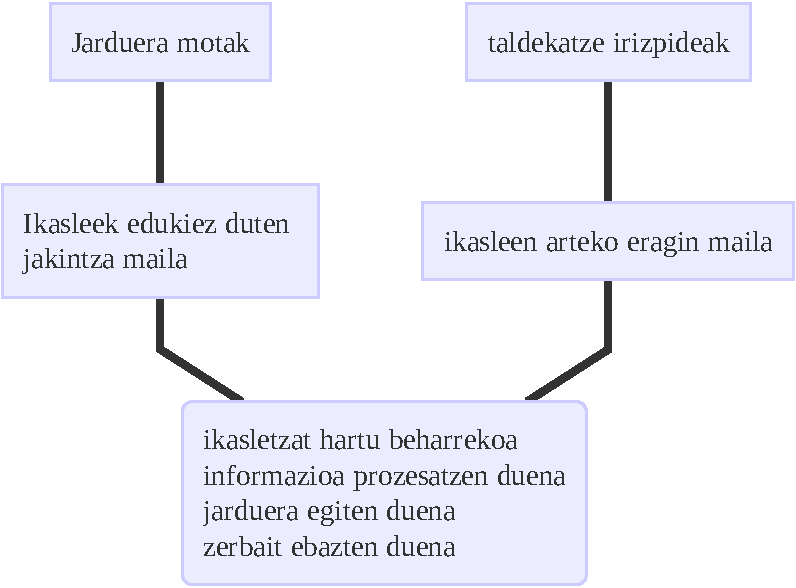
\includegraphics{bookdown-demo_files/figure-latex/unnamed-chunk-8-1.pdf}

\hypertarget{irakaslearen-zeregina}{%
\subsection{Irakaslearen zeregina}\label{irakaslearen-zeregina}}

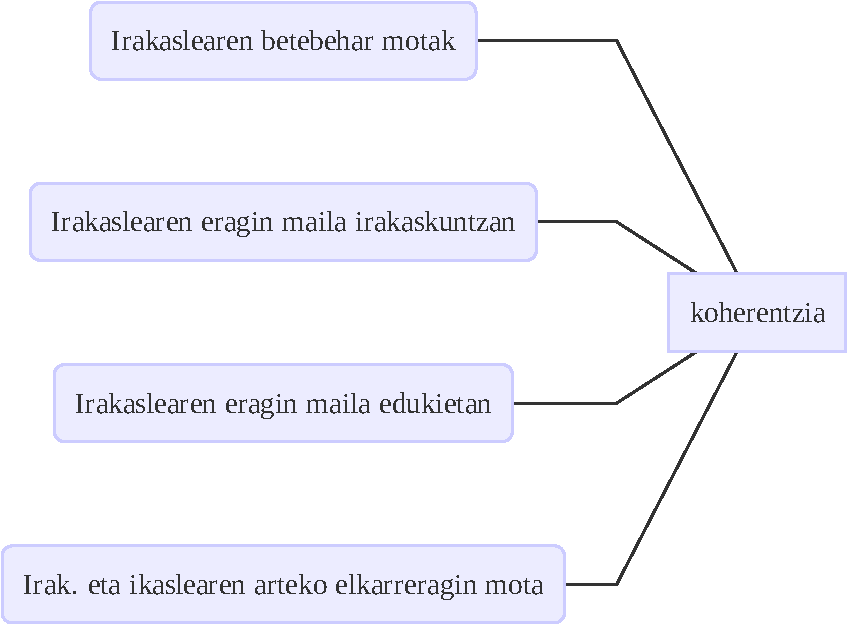
\includegraphics{bookdown-demo_files/figure-latex/unnamed-chunk-9-1.pdf}

\hypertarget{baliabide-materialak}{%
\subsection{Baliabide materialak}\label{baliabide-materialak}}

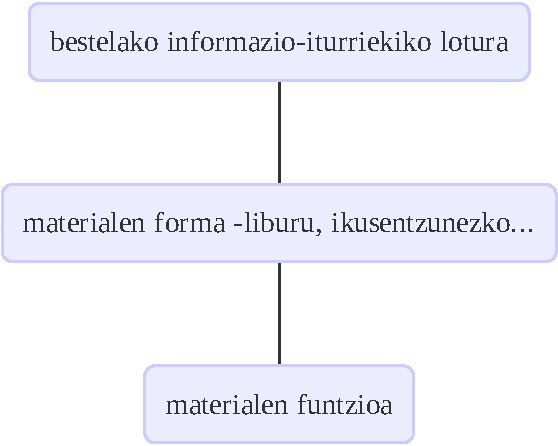
\includegraphics{bookdown-demo_files/figure-latex/unnamed-chunk-10-1.pdf}

\hypertarget{hizkuntzaren-ikaskuntza-kooperatiboa}{%
\section{Hizkuntzaren ikaskuntza kooperatiboa}\label{hizkuntzaren-ikaskuntza-kooperatiboa}}

\begin{quote}
``El aprendizaje cooperativo es una actividad de aprendizaje en grupo organizada de manera que el aprendizaje esté en dependencia del intercambio de información, socialmente estructurado, entre los alumnos distribuidos en grupos, y en el cual a cada alumno se le considera responsable de su propio aprendizaje y se le motiva para aumentar el aprendizaje de los demás.''

(Olsen y Kagan, 1992: 8)
\end{quote}

Hizkuntzen ikaskuntza komunikatiboaren ildokoa da ikaskuntza kooperatiboa. Hona zergatik:

\begin{itemize}
\tightlist
\item
  Hizkuntza era naturalean lantzen da taldean eta bakarka egiten diren jardueren bidez.
\item
  Elkarreraginaren bidez hizkuntzaren sistema lantzen da: lexikoa, hizkuntza-egiturak eta funtzio komunikatiboak.
\item
  Komunikazio- eta ikas-estrategiak lantzen dira.
\end{itemize}

\begin{center}\rule{0.5\linewidth}{0.5pt}\end{center}

\hypertarget{jardueratxoa-33}{%
\chapter*{Jarduera(txoa) (3/3)}\label{jardueratxoa-33}}
\addcontentsline{toc}{chapter}{Jarduera(txoa) (3/3)}

\textbf{Zein ikaskuntza teoria}tan oinarritu dugu gure planteamendu praktikoa; hurrengo jarreretan zuena identifikatu eta horren arabera + hemengo baliabidetxu hau erabilita \textbf{sarrera idatzi zuen Sekuentzia Didaktiko / Unitate Didaktikoari}.

\begin{quote}
Hitz egiteko jaio gara
\end{quote}

ala

\begin{quote}
Gehien erabiltzen dugun testu mota elkarrizketa da
\end{quote}

ala

\begin{quote}
Elkarrizketak kooperazio irizpideen arabera antolatu ditugu
\end{quote}

Vygotskyk eta Piagetek nabarmendu zuten 1965ean: \textbf{\emph{Gizartearekiko elkarreraginaren bidez ikasten dugu}}.

Aztertu ezaugarriok:

\begin{itemize}
\tightlist
\item
  Interdependentzia positiboa
\item
  Taldea eratzea
\item
  Bakoitzaren ardura
\item
  Gizarteko trebetasunak
\item
  Egituratzea
\end{itemize}

Orain bai: zuen lana aztertu eta sarrera polita idatzi egiozue.

\hypertarget{hizkuntzen-irakaskuntza-estrategiak}{%
\chapter{Hizkuntzen irakaskuntza estrategiak}\label{hizkuntzen-irakaskuntza-estrategiak}}

\href{../Diapoak/06_diapo_estrategiak.html}{
\includegraphics{assets/badge.png}}

Hizkuntzen ikaskuntzaren gainean hainbat zalantza eta galdera etortzen zaizkio irakasle zein ikasleari, askotan antzerako erantzuna izaten dutena

\textbf{Irakasleenak}:

\begin{quote}
Ikasle txarra da
\end{quote}

edo

\begin{quote}
Oso motibatuta dago
\end{quote}

edo

\begin{quote}
Ez dauka motibaziorik
\end{quote}

edo

\begin{quote}
Zergatik ateratzen ote ditu horrelako nota txarrak?
\end{quote}

edo

\begin{quote}
Zergatik ikasten du hain erraz horrek?
\end{quote}

\textbf{Ikasleenak}:

\begin{quote}
Ez dut ondo entzuten
\end{quote}

edo

\begin{quote}
Gogaituta nago akatsekin
\end{quote}

edo

\begin{quote}
Zaila da hizkuntza honetan aritzea!
\end{quote}

Eta asko-askotan, galdera guztien ardatza estrategiak eta motibazioak zehazten dute!

\hypertarget{testuingurua}{%
\section{Testuingurua}\label{testuingurua}}

80ko eta 90eko hamarkadetanko \textbf{eredu psikopragmatiko}ari jarraituz:

\begin{quote}
Teoria \textbf{kognitiboen} (ikaskuntzari buruzkoak) eta \textbf{konstruktibisten} garaia da, estrategiez jabetzea komunikazio egoeretan nahiz \textbf{autonomiaren} garapena lortzea izan dira helburuak. Ekintza \textbf{metakognitiboak} bultzatzen dira.

\emph{M.L. Villanueva, 1997: 82- 84}
\end{quote}

Hizkuntzak ikasten dituen ikaslea ez da subjektu pasiboa

\begin{itemize}
\tightlist
\item
  Zenbait ezaugarri propio ditu ikastunak:

  \begin{itemize}
  \tightlist
  \item
    sinismenak,
  \end{itemize}
\item
  beharrizanak,
\item
  motibazioak,
\item
  estilo kognitiboa,
\item
  izaera,
\item
  \ldots{}
\item
  Prozesu horretan gaitasunak garatzeko eta trebetasunak lantzeko zenbait prozedura egiten ditu (Cuq, 2003; Legendre, 1993; Tardif, 1992; Stern, 1983):

  \begin{itemize}
  \tightlist
  \item
    Planak
  \end{itemize}
\item
  Buruko ariketa konszienteak, ez konszienteak eta erabat konszienteak
\item
  Arazoak konpontzeko ekintza kognitiboak portaerak, ekintza funtzionalak
\end{itemize}

Prozedurok ikas-estrategiak definitzeko erabili dira

\begin{quote}
Ikasleak bere ikaskuntza era autonomoan eta aktiboan hobetzeko erabiltzen dituen prozedurak dira ikas-estrategiak

--\emph{Oxford, 1989}
\end{quote}

Egoera horiei aurre egiteko \textbf{metakognizioa}, \textbf{kontzientzia estrategikoa} eta \textbf{esperientzia praktikoa} lantzeko bidea ireki da eta honako ideia honi garrantzia ematen hasi zaio: \textbf{ikasleei ikasten irakastea} da irakasleak egin beharreko lana, bakoitzaren ikaskuntza-prozesua kontuan hartuaz eta landuaz (Roy, 1991), horretarako honako pausuak proposatzen dira:

\begin{itemize}
\tightlist
\item
  Ikasleak \textbf{ezagutu} behar ditu
\item
  Hizkuntzaren ikaskuntzaren planifikazioa egiteko ikasleek \textbf{zer helburu eta estrategia dituzten jakin} behar du.
\item
  Ikasgelako interbentzioa egiteko \textbf{zer egoera diren egokienak jakin} behar du irakasleak
\item
  \textbf{Ebaluazioa} egiteko, zer baliabide dauden jakin behar du, ikasleen aurrerapena eta emaitzak ikusteko
\end{itemize}

\hypertarget{estrategia-motak}{%
\section{Estrategia motak}\label{estrategia-motak}}

\begin{itemize}
\tightlist
\item
  Motibazio estrategiak
\item
  Ikas estrategiak
\item
  Komunikazio estrategiak
\end{itemize}

\begin{quote}
Motibazioa gaur egun irakasleek aurrean daukaten erronkarik konplexu eta handiena da, zalantza barik

--\emph{Scheidecker eta Freeman, 199: 116}
\end{quote}

\hypertarget{motibazio-estrategiak}{%
\subsection{Motibazio estrategiak}\label{motibazio-estrategiak}}

Zer diren:

\begin{quote}
Gizakiarengan helburuak kontuan hartuta portaera positiboa bultzatzen duten teknikak, nahita sortutako motibazioa eraginez.

--\emph{Dörnyei, 2003: 40}
\end{quote}

Jarraitu beharreko irizpideak:

\begin{itemize}
\tightlist
\item
  Motibaziorako oinarrizko baldintzak sortzea.
\item
  Hasierako motibazioa sortzea.
\item
  Motibazioa elikatu eta babestea.
\item
  Atzera begirako autoebaluazio positiboa bultzatzea.
\end{itemize}

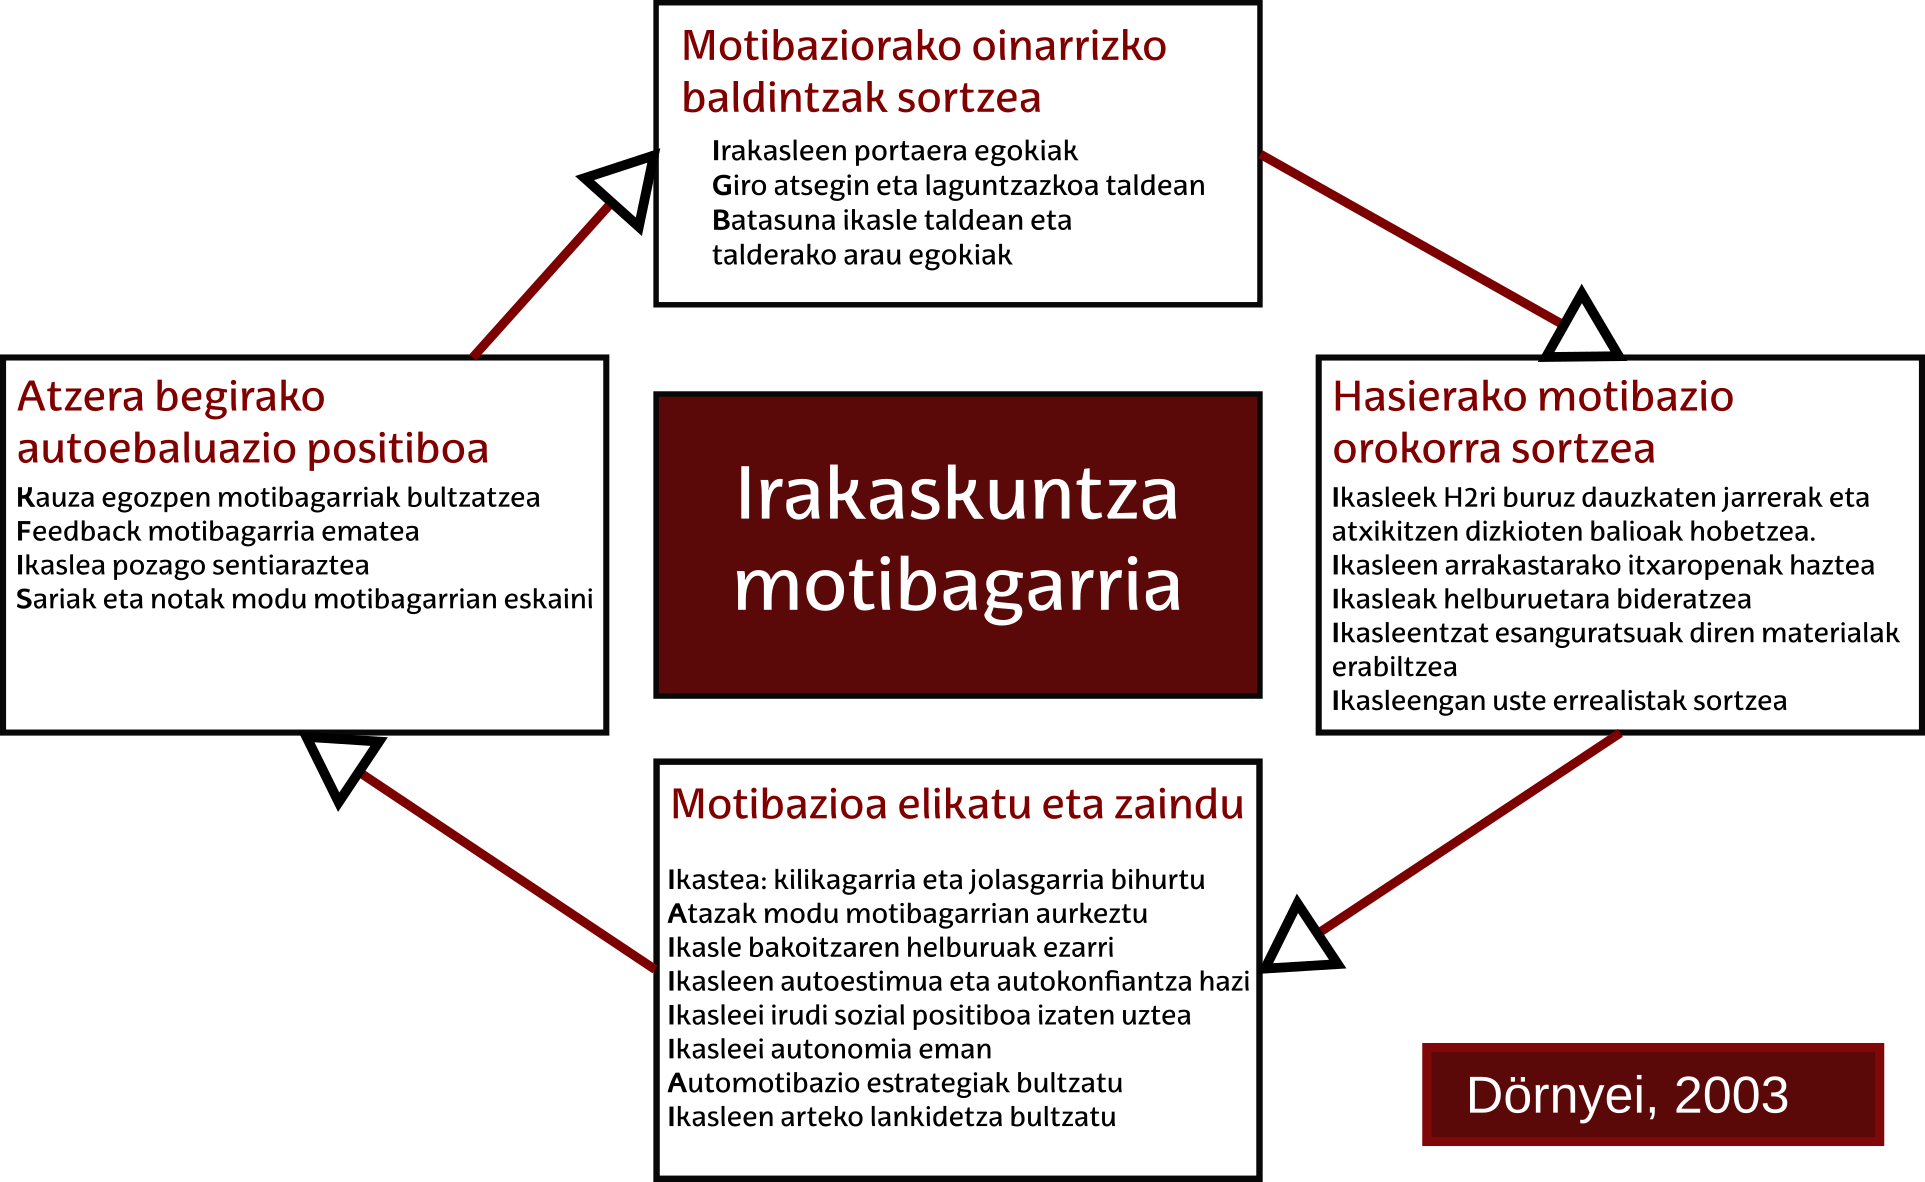
\includegraphics{assets/06-01_Irakaskuntza motibagarria.png}

\hypertarget{motibazioaren-garrantziaren-ondorioz}{%
\subsubsection{Motibazioaren garrantziaren ondorioz}\label{motibazioaren-garrantziaren-ondorioz}}

Irakaskuntzan saiatu behar dugu ikasi behar dutenen motibazioaz ere arduratzen. Horretarako Dörnyeik prestatu eta HABEk euskaratu zuen \href{https://b08normalkuntza.wikispaces.com/file/view/MOTIBAZIO+ESTRAT.pdf}{*Motibazio-estrategiak hizkuntza-ikasgelan} artikuluan eskaintzen den irakaslearentzako galdetegia erabil daiteke.

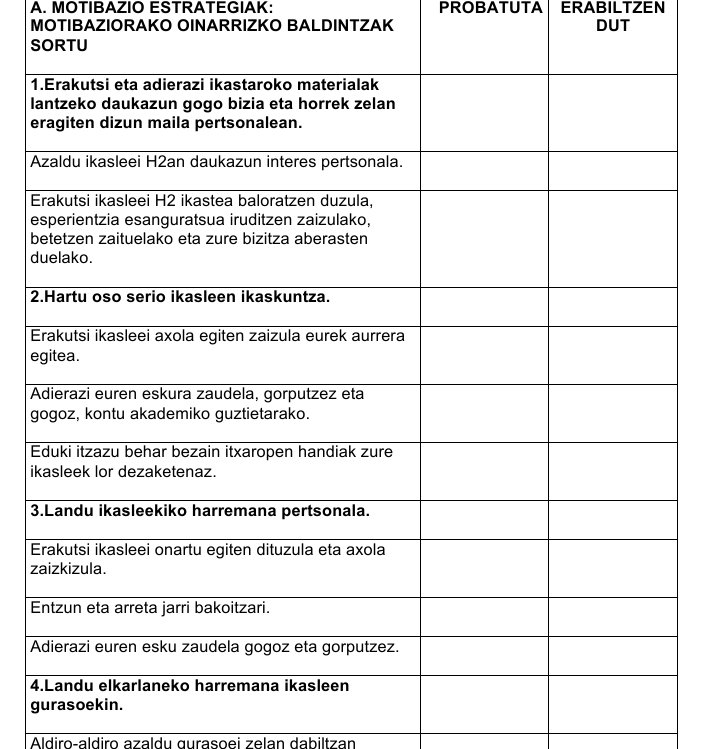
\includegraphics{assets/06-02.png}

\hypertarget{ikasteko-estrategiak-eta-komunikazio-estrategiak}{%
\subsection{Ikasteko estrategiak eta komunikazio estrategiak}\label{ikasteko-estrategiak-eta-komunikazio-estrategiak}}

Ikuskera desberdin eta osagarriak zenbaitetan.

\begin{quote}
Ikasleak komunikazioarekin erlazionatutako arazo bat duenean, eta hizkuntza baliabide nahiko ez dituenean, komunikazio-estrategiak erabiltzen ditu (parafrasia erabiltzea, laguntza eskatzea). Ikertzaile biek adierazten dute komunikazio-estrategien bidez ikasten dela eta, horregatik, bi helburu izan ditzaketela: alde batetik, ikastea; eta bestetik, komunikatzea.

--\emph{Faerch eta Kasper (1980)}
\end{quote}

Oxford-ek (1990), ordea, ez du uste \emph{komunikazio-estrategiak} terminoa erabiltzea egokia denik, euren funtzioa ikas-prozesuan ez dagoelako argi eta uste du ikaskuntzan laguntzaile bezala besterik ez dutela jokatzen, hau da, ez direla erabakigarriak hizkuntza ikasteko orduan, lagundu egiten dute besterik ez.

O'Malley eta Chamot-ek (1990), aldiz, komunikazio-estrategiek duten garrantzia ez dute ukatzen, eta bi funtzio bereizten dituzte: bata ikastea da, \textbf{ikas-estrategia}, eta bestea komunikazioa, \textbf{komunikazio-estrategia}.

\hypertarget{adibidea-plumber}{%
\subsubsection{\texorpdfstring{Adibidea: \emph{plumber}}{Adibidea: plumber}}\label{adibidea-plumber}}

Gerta daiteke ikasleren batek plumber hitza ez ezagutzea eta hori komunikazio-ekintza batean erabili behar izatea.

Zer egingo du ikasleak?

Komunikazio-estrategia bat erabili dezake, hala nola, parafrasia, \emph{hoditeria konpontzen duen langilea}, adierazi nahi duena esateko.

Momentu zehatz horretarako lagungarri izango zaio, baina helburua hitz hori ikastea baldin bada, beste estrategia bat erabili beharko du. Esate baterako, hiztegian bilatuko du hitza, solaskideari hitza errepikatzea eskatuko dio edota koadernoan idatziko du ez ahazteko (ikas-estrategiak).

Hainbat estrategia erabili ditzake hitza barneratzeko. Estrategia-mota bat edo bestea erabiltzea \textbf{ikas-estiloa}ren araberakoa izango da.

\hypertarget{ikas-estiloak}{%
\subsection{Ikas estiloak}\label{ikas-estiloak}}

Zer dira? Ikas-estrategiekin zerikusirik ote dute?

Erabili diren definizio batzuk dira hurrengoak:

\begin{quote}
Informazioa prozesatzeko erak

--\emph{Smith (1988)}
\end{quote}

\begin{quote}
Ikasteko gaitasunak genetikak, inguruak eta norberaren eskarmentuak baldintzatuak dauden ezaugarriak

--\emph{Kolb (1984)}
\end{quote}

\begin{quote}
Ezaugarri afektiboen, joera psikologikoen eta ezagutza-ezaugarrien multzoa

--\emph{Rumiche-Chávarry (2013)}
\end{quote}

Argigarria da Estebanek eta Ruizezk 1996an zehaztutakoa:

\begin{quote}
Ikas estrategien bidez, ikas estiloak antzeman ditzakegu

--\emph{Esteban eta Ruiz (1996:121-122)}
\end{quote}

\hypertarget{ikas-estiloak-1}{%
\subsubsection{Ikas-estiloak}\label{ikas-estiloak-1}}

Aurrez Oxfordek egindako lanean (1993) oinarrituta, Pikabeak (2002) egindako zerrenda dakargu, ikasleen ikas-estiloen hurrenkera bat aurkezteko.

\begin{itemize}
\tightlist
\item
  Zentzumenak erabiltzen dituzten estiloak
\item
  Ikuslea
  Ikusiz hobeto ikasten duenari deritzo: bideoak, grafikoak, liburuak
\item
  Entzulea
  Entzunez eta mintzatuz hobeto ikasten duenari deritzo: eztabaidak, audiozintak, rol-jokoak\ldots{}
\item
  Egilea
  Ekinaz ikasten hobeto ikasten duenari deritzo: mugimenduzko jokoak, esku-lanak, etab.
\item
  Jendearekin duten \textbf{harremanaren} araberakoa:

  \begin{itemize}
  \tightlist
  \item
    Konparakoia.\\
    Gustuko ditu hartuemanak, eztabaidak, rol-jokoak\ldots{}
  \end{itemize}
\item
  Barnerakoia\\
  Gustuko du bakarka, bere kasa edo gertukoekin ikastea
\item
  Norabideen arabera
\item
  Intuitiboa
  Gustuko ditu abstrakzioa, orokortzea eta geroaldia
\item
  Zehatza eta sekuentziala
  Gustuko ditu zehaztasuna, orainaldia eta urratsez urrats aritzea.
\item
  Ariketa moten arabera
\item
  Ariketa itxi zalea
  Gustuko ditu ariketa zehatz eta oso arautuak: azpimarratzea, egituraketak, planifikazioak\ldots{}
\item
  Ariketa ireki zalea
  Gustuko ditu egoera ez egituratuak: informazioa jasotzea, era ez sistematikoan ikastea\ldots{}
\item
  Ideiak tratatzeko moduaren arabera
\item
  Globala
  Globaltasuna ezagutzea du gustuko: ideia nagusiak biltzea, esanahiak asmatzea, istorioen hasierak edo bukaerak asmatzea; hitz guztiak ezagutu ez arren komunikatzea du gustuko.
\item
  Analitikoa
  Gustuko ditu logika eta xehetasunak: esaldi eta hitzak zatitu eta txikitzea, arauak aztertzea eta alikatzea
\end{itemize}

\hypertarget{ikas-estrategiak}{%
\subsubsection{Ikas-estrategiak}\label{ikas-estrategiak}}

Horiek zerrendatzeko O'Malleyk eta Chamotek (1990) egindako tipologia erabiliko dugu:

\begin{itemize}
\tightlist
\item
  Estrategia metakognitiboak:

  \begin{itemize}
  \tightlist
  \item
    Ikas-prozesuari buruzko gogoeta.
  \item
    Ikasteko prestakuntza.
  \item
    Ikas-ekintzen kontrola.
  \item
    Autoebaluazioa.
  \end{itemize}
\item
  Estrategia kognitiboak:

  \begin{itemize}
  \tightlist
  \item
    Gaiarekiko elkarreragina.
  \item
    Gaiaren manipulazioa.
  \end{itemize}
\item
  Estragegia sozio-afektiboak:

  \begin{itemize}
  \tightlist
  \item
    Beste pertsona batekiko elkarreragina.
  \item
    Alde afektiboaren kontrola.
  \end{itemize}
\end{itemize}

\begin{center}\rule{0.5\linewidth}{0.5pt}\end{center}

\hypertarget{klasean-egin-beharreko-ariketa}{%
\section*{Klasean egin beharreko ariketa}\label{klasean-egin-beharreko-ariketa}}
\addcontentsline{toc}{section}{Klasean egin beharreko ariketa}

Teorian eta galdetegiko erantzunetan oinarrituta, erantzun galderok:

\begin{enumerate}
\def\labelenumi{\arabic{enumi}.}
\tightlist
\item
  Zein da taldean gailentzen den ikas-estiloa?
\item
  Zeintzuk ikas-estrategia erabiltzen dituzue gehien?
  Eta gutxien?
\end{enumerate}

Sortu grafikoa eta azaldu.

\begin{center}\rule{0.5\linewidth}{0.5pt}\end{center}

\hypertarget{ikas-estrategiak-lantzeko-proposamenak}{%
\subsection{Ikas-estrategiak lantzeko proposamenak}\label{ikas-estrategiak-lantzeko-proposamenak}}

Proposamen ugarien artean, hona batzuk, Etxeberria eta Garay (2012) artikulutik ekarrita:

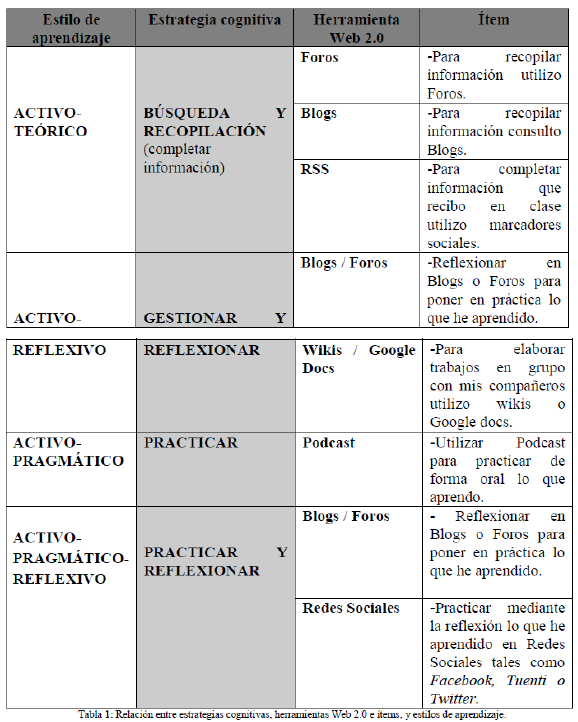
\includegraphics{assets/06-03.png}

Beste proposamen bat egin zuten O'Malleyk eta Chamotek (1994)

\begin{description}
\tightlist
\item[Prestakuntza fasea]
Ezagutza metakognitiboa garatu.
Hizkutza-ariketa laburrak taldean egin eta nola egin duten azaldu.
\item[Aurkezpena]
Ikas-estrategiak modu esplizituan irakasten dira, zer diren eta nola erabili.
\item[Praktika]
Ariketen bidez ikas-estrategien erabilera jarduera ezberdinetan txertatzen da.
\item[Ebaluazioa]
Galdeketa erantzun
\end{description}

--

Fase horietako adibide batzuk izan litezke:

\hypertarget{aurkezpena}{%
\paragraph{Aurkezpena:}\label{aurkezpena}}

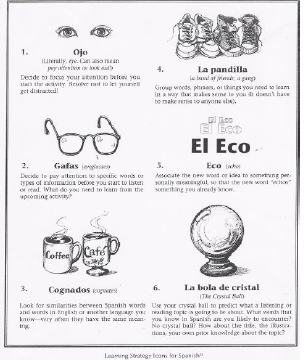
\includegraphics{assets/06-04.png}

A. Chamot eta M. O'Malley, 1994

\hypertarget{praktikarako-proposamena}{%
\paragraph{Praktikarako proposamena:}\label{praktikarako-proposamena}}

\begin{itemize}
\tightlist
\item
  Ikaskuntza kooperatiboa
\item
  Berdinen arteko tutoretza
\item
  Zientzia esperimentuak
\item
  Matematika problemak
\item
  Ikerkuntza proiektuak
\item
  Erreportajeak
\item
  Literatura
\end{itemize}

\hypertarget{adibideak}{%
\paragraph{Adibideak}\label{adibideak}}

\textbf{Topatu zure bidea jarduera}

Entzutezko ulermena lantzen den ariketa honetan mapa batean ibilbide bat adierazteko eskatuko zaie ikasleei.

Ariketa hau egiteko estrategia hauek erabil daitezke:

\begin{itemize}
\tightlist
\item
  zuzeneko estrategiak:

  \begin{itemize}
  \tightlist
  \item
    praktikatzea
  \item
    galdetzea
  \item
    irudiak erabiltzea
  \end{itemize}
\item
  zeharkako estrategiak

  \begin{itemize}
  \tightlist
  \item
    arreta jartzea
  \end{itemize}
\end{itemize}

\begin{description}
\tightlist
\item[Baliabide materiala]
mapa baten fotokopia
\item[Denbora]
20 minutu
\item[Nola egin]
leku baten mapa lortu. Irakasleak bere mapan ibilbide batmarkatuko du, gero ikasleei nora joan behar duten azalduko dieinguruko lekuak, jendea\ldots{} aipatuz.
\end{description}

Oxford, 1989: 106

\textbf{Esanahia asmatzea irakurtzen ari diren testu batean}.

Ariketa honek ikasleei irakurtzen ari diren testu baten esanahia asmatzen laguntzeaz gain, nolaasmatu duten azaltzen ere laguntzen die.

\begin{description}
\tightlist
\item[Baliabide materiala]
irakurtzeko testu-zatiak.
\item[Denbora]
30-50 minutu irauten du.
\item[Nola egin]
irakasleak ikasleei asmakizunak hainbat hizkuntzatan egingo dituztela azalduko die.
Gero,orri bat instrukzioekin eta irakurri behar dituzten testu-zatiekin emango die.
Ikasleak, testu-zatiak irakurri ondoren, esanahi orokorra asmatzen ahaleginduko dira.
Bukatzeko, ikasleek R. Oxford-ekproposatzen dituen galdera hauek erantzun beharko dituzte:
\end{description}

\begin{quote}
\begin{enumerate}
\def\labelenumi{\arabic{enumi}.}
\tightlist
\item
  Summarize the meaning of each passage in one sentence
\item
  How well did you understand the meaning of each the passages above
  Which passages gave you the most trouble, and why?
\item
  If you did not understand certain words, which ones werw they?
\item
  Did you try to guess the meaning of unknown or unclear words?
  If so, how often?
  What are some examples of wunknown words you were able to guess?
  Whatt information did you use to make your guesses?
\item
  What other information sources might you hvave used to guess the meanings?
  List as many sources as you can think of.
\item
  Did you need tto know (or guess) the meanings of all the words in a passage in order to know (or guess) the overall meaning of the whole passage? In other words, do you need to get the details in order to get the general idea?
\end{enumerate}
\end{quote}

Oxford, 1989: 112

\textbf{Irudiekin asmatzen}
Ariketa honek ikasleari irudiak erabiliz asmatzeko estrategiak praktikatzen lagunduko dio.

\begin{description}
\tightlist
\item[Baliabide materiala]
hitzik gabeko komiki bat.
\item[Denbora]
10-30 minututan egin daitekeen ariketa da, baina erabiltzen diren komikien kopuruaren arabera, denbora hori aldakorra izan daiteke.
\item[Nola egin]
ikasleek hitzik gabeko komikietako hutsuneak xede hizkuntzan bete beharko dituzte. Irudiak hutsuneak betetzeko orduan erabilgarriak izan daitezke.
\end{description}

Oxford, 1989: 112

\hypertarget{erreferentziak}{%
\section{Erreferentziak}\label{erreferentziak}}

Chamot, A. U., \& O'Malley, J. M. (1994). \emph{The CALLA handbook: implementing the cognitive academic language learning approach /}. Reading, Mass.: Addison-Wesley Pub. Co.,.

Cuq, J.-P. (2003). \emph{Dictionnaire de didactique du français langue étrangère et seconde}. Paris: Clé International.

Cyr, P. (2000). \emph{Estrategiak bigarren hizkuntza baten irakaskuntzan}. (B. Urkizu, Itzul.). Donostia: Habe.

Dörnyei, Z. (2003). \emph{Motibazio-estrategiak hizkuntz ikasgelan}. (A. I. Morales, Itzul.). Donostia: Habe.

Etxebarria, A. (2008). Estrategiak hizkuntzen ikaskuntzan eta irakaskuntzan: M. O'Malley-ren eta A. Chamot-en ekarpena. \emph{Litterae vasconicae: euskeraren iker atalak}, (10), 241--279.

Etxebarria, A., \& Garay, U. (2012). Estilo de aprendizaje basado en el uso de estrategias cognitivas por medio de aplicaciones virtuales. Learning style based on the use of cognitive strategies by virtual applications. In \emph{V Congreso Mundial de Estilos de Aprendizaje}. Santander. Berreskuratua \url{https://dialnet.unirioja.es/servlet/articulo?codigo=4636744}-(e)tik

Færch, C., \& Kasper, G. (1980). Processes and Strategies in Foreign Language Learning and Communication. \emph{Interlanguage Studies Bulletin}, \emph{5}(1), 47--118.

Kolb, D. (1985). \emph{Learning style inventory}. Boston, MA: McBer and Company.

Legendre, R. (1993). \emph{Dictionnaire actuel de l'éducation}. Paris: Guérin. Berreskuratua \url{https://dspacecdc-test.inlibro.net/xmlui/handle/11515/5065} -(e)tik

Oxford, R. L. (1990). \emph{Language Learning Strategies: What Every Teacher Should Know} (1. arg.). Heinle ELT. Berreskuratua \url{http://gen.lib.rus.ec/book/index.php?md5=D35AD86CE0610D7EC0AD25197FB3BBE4} -(e)tik

Pikabea, I. (2002). \emph{Ikasle helduen ikas-estiloak eta ikas-estrategiak euskararen ikaskuntzan eta erabilera ohiturak ikasgelatik kanpo: interventzio-programa bat} (PhD). Euskal Herriko Unibertsitatea, Donostia. Berreskuratua \url{http://www.euskara.euskadi.net/appcont/tesisDoctoral/PDFak/Inaki_Pikabea_TESI.pdf}-(e)tik

recherche, résultats de. (2003). \emph{Dictionnaire de didactique du français langue étran- Livre}. Paris: Clé International.

Ruiz, J. C., \& Albert, M. E. (1996). Presentación del tema monográfico ¿Estrategias y estilos de aprendizaje?. \emph{Anales de psicología}, \emph{12}(2), 121--122.

Rumiche-Chávarry, R. del P. (2013). \emph{Los estilos de aprendizaje y el uso de la plataforma virtual por los estudiantes de la facultad de educación de la universidad católica Santo Toribio de Mogrovejo} (Doktorego-tesia). Universidad de Málaga. Berreskuratua \url{https://dialnet.unirioja.es/servlet/tesis?codigo=132172}-(e)tik

Scheidecker, D., \& Freeman, W. (1999). \emph{Bringing Out the Best in Students: How Legendary Teachers Motivate Kids}. New York: Skyhorse Publishing.

Smith, R. M. (1984). \emph{Learning How to Learn}. Milton Keynes: Open University Press.

Stern, H. H. (1984). \emph{Fundamental concepts of language teaching}. Oxford: Oxford University Press.

Tardif, J. (1992). \emph{Pour un enseignement stratégique. L'apport de la psychologie cognitive}. Montreal: Logiques.

Villanueva, M. L., \& Navarro, I. (1997). \emph{Los estilos de aprendizaje de lenguas: un estudio sobre las representaciones culturales y las interacciones de enseñanza-aprendizaje}. Castellón: Universitat Jaume I.

\hypertarget{laugarren-jarduera}{%
\section*{Laugarren jarduera}\label{laugarren-jarduera}}
\addcontentsline{toc}{section}{Laugarren jarduera}

Jarduera hau klasean azalduko da ondo. Baina, despistatuentzat lehenengo pausuak:

\begin{enumerate}
\def\labelenumi{\arabic{enumi}.}
\tightlist
\item
  Aberiguatu (eta definitu)
\end{enumerate}

\begin{itemize}
\tightlist
\item
  Zer den \emph{bideotutoriala}
\item
  Zein ezaugarri izaten dituen
\item
  Nolako motak dauden
\item
  Era desberdinetakoen adibide itxurosoak aurkitu
\end{itemize}

\end{document}
